\documentclass[11pt]{article}

    \usepackage[breakable]{tcolorbox}
    \usepackage{parskip} % Stop auto-indenting (to mimic markdown behaviour)
    
    \usepackage{iftex}
    \ifPDFTeX
    	\usepackage[T1]{fontenc}
    	\usepackage{mathpazo}
    \else
    	\usepackage{fontspec}
    \fi

    % Basic figure setup, for now with no caption control since it's done
    % automatically by Pandoc (which extracts ![](path) syntax from Markdown).
    \usepackage{graphicx}
    % Maintain compatibility with old templates. Remove in nbconvert 6.0
    \let\Oldincludegraphics\includegraphics
    % Ensure that by default, figures have no caption (until we provide a
    % proper Figure object with a Caption API and a way to capture that
    % in the conversion process - todo).
    \usepackage{caption}
    \DeclareCaptionFormat{nocaption}{}
    \captionsetup{format=nocaption,aboveskip=0pt,belowskip=0pt}

    \usepackage[Export]{adjustbox} % Used to constrain images to a maximum size
    \adjustboxset{max size={0.9\linewidth}{0.9\paperheight}}
    \usepackage{float}
    \floatplacement{figure}{H} % forces figures to be placed at the correct location
    \usepackage{xcolor} % Allow colors to be defined
    \usepackage{enumerate} % Needed for markdown enumerations to work
    \usepackage{geometry} % Used to adjust the document margins
    \usepackage{amsmath} % Equations
    \usepackage{amssymb} % Equations
    \usepackage{textcomp} % defines textquotesingle
    % Hack from http://tex.stackexchange.com/a/47451/13684:
    \AtBeginDocument{%
        \def\PYZsq{\textquotesingle}% Upright quotes in Pygmentized code
    }
    \usepackage{upquote} % Upright quotes for verbatim code
    \usepackage{eurosym} % defines \euro
    \usepackage[mathletters]{ucs} % Extended unicode (utf-8) support
    \usepackage{fancyvrb} % verbatim replacement that allows latex
    \usepackage{grffile} % extends the file name processing of package graphics 
                         % to support a larger range
    \makeatletter % fix for grffile with XeLaTeX
    \def\Gread@@xetex#1{%
      \IfFileExists{"\Gin@base".bb}%
      {\Gread@eps{\Gin@base.bb}}%
      {\Gread@@xetex@aux#1}%
    }
    \makeatother

    % The hyperref package gives us a pdf with properly built
    % internal navigation ('pdf bookmarks' for the table of contents,
    % internal cross-reference links, web links for URLs, etc.)
    \usepackage{hyperref}
    % The default LaTeX title has an obnoxious amount of whitespace. By default,
    % titling removes some of it. It also provides customization options.
    \usepackage{titling}
    \usepackage{longtable} % longtable support required by pandoc >1.10
    \usepackage{booktabs}  % table support for pandoc > 1.12.2
    \usepackage[inline]{enumitem} % IRkernel/repr support (it uses the enumerate* environment)
    \usepackage[normalem]{ulem} % ulem is needed to support strikethroughs (\sout)
                                % normalem makes italics be italics, not underlines
    \usepackage{mathrsfs}
    

    
    % Colors for the hyperref package
    \definecolor{urlcolor}{rgb}{0,.145,.698}
    \definecolor{linkcolor}{rgb}{.71,0.21,0.01}
    \definecolor{citecolor}{rgb}{.12,.54,.11}

    % ANSI colors
    \definecolor{ansi-black}{HTML}{3E424D}
    \definecolor{ansi-black-intense}{HTML}{282C36}
    \definecolor{ansi-red}{HTML}{E75C58}
    \definecolor{ansi-red-intense}{HTML}{B22B31}
    \definecolor{ansi-green}{HTML}{00A250}
    \definecolor{ansi-green-intense}{HTML}{007427}
    \definecolor{ansi-yellow}{HTML}{DDB62B}
    \definecolor{ansi-yellow-intense}{HTML}{B27D12}
    \definecolor{ansi-blue}{HTML}{208FFB}
    \definecolor{ansi-blue-intense}{HTML}{0065CA}
    \definecolor{ansi-magenta}{HTML}{D160C4}
    \definecolor{ansi-magenta-intense}{HTML}{A03196}
    \definecolor{ansi-cyan}{HTML}{60C6C8}
    \definecolor{ansi-cyan-intense}{HTML}{258F8F}
    \definecolor{ansi-white}{HTML}{C5C1B4}
    \definecolor{ansi-white-intense}{HTML}{A1A6B2}
    \definecolor{ansi-default-inverse-fg}{HTML}{FFFFFF}
    \definecolor{ansi-default-inverse-bg}{HTML}{000000}

    % commands and environments needed by pandoc snippets
    % extracted from the output of `pandoc -s`
    \providecommand{\tightlist}{%
      \setlength{\itemsep}{0pt}\setlength{\parskip}{0pt}}
    \DefineVerbatimEnvironment{Highlighting}{Verbatim}{commandchars=\\\{\}}
    % Add ',fontsize=\small' for more characters per line
    \newenvironment{Shaded}{}{}
    \newcommand{\KeywordTok}[1]{\textcolor[rgb]{0.00,0.44,0.13}{\textbf{{#1}}}}
    \newcommand{\DataTypeTok}[1]{\textcolor[rgb]{0.56,0.13,0.00}{{#1}}}
    \newcommand{\DecValTok}[1]{\textcolor[rgb]{0.25,0.63,0.44}{{#1}}}
    \newcommand{\BaseNTok}[1]{\textcolor[rgb]{0.25,0.63,0.44}{{#1}}}
    \newcommand{\FloatTok}[1]{\textcolor[rgb]{0.25,0.63,0.44}{{#1}}}
    \newcommand{\CharTok}[1]{\textcolor[rgb]{0.25,0.44,0.63}{{#1}}}
    \newcommand{\StringTok}[1]{\textcolor[rgb]{0.25,0.44,0.63}{{#1}}}
    \newcommand{\CommentTok}[1]{\textcolor[rgb]{0.38,0.63,0.69}{\textit{{#1}}}}
    \newcommand{\OtherTok}[1]{\textcolor[rgb]{0.00,0.44,0.13}{{#1}}}
    \newcommand{\AlertTok}[1]{\textcolor[rgb]{1.00,0.00,0.00}{\textbf{{#1}}}}
    \newcommand{\FunctionTok}[1]{\textcolor[rgb]{0.02,0.16,0.49}{{#1}}}
    \newcommand{\RegionMarkerTok}[1]{{#1}}
    \newcommand{\ErrorTok}[1]{\textcolor[rgb]{1.00,0.00,0.00}{\textbf{{#1}}}}
    \newcommand{\NormalTok}[1]{{#1}}
    
    % Additional commands for more recent versions of Pandoc
    \newcommand{\ConstantTok}[1]{\textcolor[rgb]{0.53,0.00,0.00}{{#1}}}
    \newcommand{\SpecialCharTok}[1]{\textcolor[rgb]{0.25,0.44,0.63}{{#1}}}
    \newcommand{\VerbatimStringTok}[1]{\textcolor[rgb]{0.25,0.44,0.63}{{#1}}}
    \newcommand{\SpecialStringTok}[1]{\textcolor[rgb]{0.73,0.40,0.53}{{#1}}}
    \newcommand{\ImportTok}[1]{{#1}}
    \newcommand{\DocumentationTok}[1]{\textcolor[rgb]{0.73,0.13,0.13}{\textit{{#1}}}}
    \newcommand{\AnnotationTok}[1]{\textcolor[rgb]{0.38,0.63,0.69}{\textbf{\textit{{#1}}}}}
    \newcommand{\CommentVarTok}[1]{\textcolor[rgb]{0.38,0.63,0.69}{\textbf{\textit{{#1}}}}}
    \newcommand{\VariableTok}[1]{\textcolor[rgb]{0.10,0.09,0.49}{{#1}}}
    \newcommand{\ControlFlowTok}[1]{\textcolor[rgb]{0.00,0.44,0.13}{\textbf{{#1}}}}
    \newcommand{\OperatorTok}[1]{\textcolor[rgb]{0.40,0.40,0.40}{{#1}}}
    \newcommand{\BuiltInTok}[1]{{#1}}
    \newcommand{\ExtensionTok}[1]{{#1}}
    \newcommand{\PreprocessorTok}[1]{\textcolor[rgb]{0.74,0.48,0.00}{{#1}}}
    \newcommand{\AttributeTok}[1]{\textcolor[rgb]{0.49,0.56,0.16}{{#1}}}
    \newcommand{\InformationTok}[1]{\textcolor[rgb]{0.38,0.63,0.69}{\textbf{\textit{{#1}}}}}
    \newcommand{\WarningTok}[1]{\textcolor[rgb]{0.38,0.63,0.69}{\textbf{\textit{{#1}}}}}
    
    
    % Define a nice break command that doesn't care if a line doesn't already
    % exist.
    \def\br{\hspace*{\fill} \\* }
    % Math Jax compatibility definitions
    \def\gt{>}
    \def\lt{<}
    \let\Oldtex\TeX
    \let\Oldlatex\LaTeX
    \renewcommand{\TeX}{\textrm{\Oldtex}}
    \renewcommand{\LaTeX}{\textrm{\Oldlatex}}
    % Document parameters
    % Document title
    \title{HW2}
    
    
    
    
    
% Pygments definitions
\makeatletter
\def\PY@reset{\let\PY@it=\relax \let\PY@bf=\relax%
    \let\PY@ul=\relax \let\PY@tc=\relax%
    \let\PY@bc=\relax \let\PY@ff=\relax}
\def\PY@tok#1{\csname PY@tok@#1\endcsname}
\def\PY@toks#1+{\ifx\relax#1\empty\else%
    \PY@tok{#1}\expandafter\PY@toks\fi}
\def\PY@do#1{\PY@bc{\PY@tc{\PY@ul{%
    \PY@it{\PY@bf{\PY@ff{#1}}}}}}}
\def\PY#1#2{\PY@reset\PY@toks#1+\relax+\PY@do{#2}}

\expandafter\def\csname PY@tok@gd\endcsname{\def\PY@tc##1{\textcolor[rgb]{0.63,0.00,0.00}{##1}}}
\expandafter\def\csname PY@tok@gu\endcsname{\let\PY@bf=\textbf\def\PY@tc##1{\textcolor[rgb]{0.50,0.00,0.50}{##1}}}
\expandafter\def\csname PY@tok@gt\endcsname{\def\PY@tc##1{\textcolor[rgb]{0.00,0.27,0.87}{##1}}}
\expandafter\def\csname PY@tok@gs\endcsname{\let\PY@bf=\textbf}
\expandafter\def\csname PY@tok@gr\endcsname{\def\PY@tc##1{\textcolor[rgb]{1.00,0.00,0.00}{##1}}}
\expandafter\def\csname PY@tok@cm\endcsname{\let\PY@it=\textit\def\PY@tc##1{\textcolor[rgb]{0.25,0.50,0.50}{##1}}}
\expandafter\def\csname PY@tok@vg\endcsname{\def\PY@tc##1{\textcolor[rgb]{0.10,0.09,0.49}{##1}}}
\expandafter\def\csname PY@tok@vi\endcsname{\def\PY@tc##1{\textcolor[rgb]{0.10,0.09,0.49}{##1}}}
\expandafter\def\csname PY@tok@vm\endcsname{\def\PY@tc##1{\textcolor[rgb]{0.10,0.09,0.49}{##1}}}
\expandafter\def\csname PY@tok@mh\endcsname{\def\PY@tc##1{\textcolor[rgb]{0.40,0.40,0.40}{##1}}}
\expandafter\def\csname PY@tok@cs\endcsname{\let\PY@it=\textit\def\PY@tc##1{\textcolor[rgb]{0.25,0.50,0.50}{##1}}}
\expandafter\def\csname PY@tok@ge\endcsname{\let\PY@it=\textit}
\expandafter\def\csname PY@tok@vc\endcsname{\def\PY@tc##1{\textcolor[rgb]{0.10,0.09,0.49}{##1}}}
\expandafter\def\csname PY@tok@il\endcsname{\def\PY@tc##1{\textcolor[rgb]{0.40,0.40,0.40}{##1}}}
\expandafter\def\csname PY@tok@go\endcsname{\def\PY@tc##1{\textcolor[rgb]{0.53,0.53,0.53}{##1}}}
\expandafter\def\csname PY@tok@cp\endcsname{\def\PY@tc##1{\textcolor[rgb]{0.74,0.48,0.00}{##1}}}
\expandafter\def\csname PY@tok@gi\endcsname{\def\PY@tc##1{\textcolor[rgb]{0.00,0.63,0.00}{##1}}}
\expandafter\def\csname PY@tok@gh\endcsname{\let\PY@bf=\textbf\def\PY@tc##1{\textcolor[rgb]{0.00,0.00,0.50}{##1}}}
\expandafter\def\csname PY@tok@ni\endcsname{\let\PY@bf=\textbf\def\PY@tc##1{\textcolor[rgb]{0.60,0.60,0.60}{##1}}}
\expandafter\def\csname PY@tok@nl\endcsname{\def\PY@tc##1{\textcolor[rgb]{0.63,0.63,0.00}{##1}}}
\expandafter\def\csname PY@tok@nn\endcsname{\let\PY@bf=\textbf\def\PY@tc##1{\textcolor[rgb]{0.00,0.00,1.00}{##1}}}
\expandafter\def\csname PY@tok@no\endcsname{\def\PY@tc##1{\textcolor[rgb]{0.53,0.00,0.00}{##1}}}
\expandafter\def\csname PY@tok@na\endcsname{\def\PY@tc##1{\textcolor[rgb]{0.49,0.56,0.16}{##1}}}
\expandafter\def\csname PY@tok@nb\endcsname{\def\PY@tc##1{\textcolor[rgb]{0.00,0.50,0.00}{##1}}}
\expandafter\def\csname PY@tok@nc\endcsname{\let\PY@bf=\textbf\def\PY@tc##1{\textcolor[rgb]{0.00,0.00,1.00}{##1}}}
\expandafter\def\csname PY@tok@nd\endcsname{\def\PY@tc##1{\textcolor[rgb]{0.67,0.13,1.00}{##1}}}
\expandafter\def\csname PY@tok@ne\endcsname{\let\PY@bf=\textbf\def\PY@tc##1{\textcolor[rgb]{0.82,0.25,0.23}{##1}}}
\expandafter\def\csname PY@tok@nf\endcsname{\def\PY@tc##1{\textcolor[rgb]{0.00,0.00,1.00}{##1}}}
\expandafter\def\csname PY@tok@si\endcsname{\let\PY@bf=\textbf\def\PY@tc##1{\textcolor[rgb]{0.73,0.40,0.53}{##1}}}
\expandafter\def\csname PY@tok@s2\endcsname{\def\PY@tc##1{\textcolor[rgb]{0.73,0.13,0.13}{##1}}}
\expandafter\def\csname PY@tok@nt\endcsname{\let\PY@bf=\textbf\def\PY@tc##1{\textcolor[rgb]{0.00,0.50,0.00}{##1}}}
\expandafter\def\csname PY@tok@nv\endcsname{\def\PY@tc##1{\textcolor[rgb]{0.10,0.09,0.49}{##1}}}
\expandafter\def\csname PY@tok@s1\endcsname{\def\PY@tc##1{\textcolor[rgb]{0.73,0.13,0.13}{##1}}}
\expandafter\def\csname PY@tok@dl\endcsname{\def\PY@tc##1{\textcolor[rgb]{0.73,0.13,0.13}{##1}}}
\expandafter\def\csname PY@tok@ch\endcsname{\let\PY@it=\textit\def\PY@tc##1{\textcolor[rgb]{0.25,0.50,0.50}{##1}}}
\expandafter\def\csname PY@tok@m\endcsname{\def\PY@tc##1{\textcolor[rgb]{0.40,0.40,0.40}{##1}}}
\expandafter\def\csname PY@tok@gp\endcsname{\let\PY@bf=\textbf\def\PY@tc##1{\textcolor[rgb]{0.00,0.00,0.50}{##1}}}
\expandafter\def\csname PY@tok@sh\endcsname{\def\PY@tc##1{\textcolor[rgb]{0.73,0.13,0.13}{##1}}}
\expandafter\def\csname PY@tok@ow\endcsname{\let\PY@bf=\textbf\def\PY@tc##1{\textcolor[rgb]{0.67,0.13,1.00}{##1}}}
\expandafter\def\csname PY@tok@sx\endcsname{\def\PY@tc##1{\textcolor[rgb]{0.00,0.50,0.00}{##1}}}
\expandafter\def\csname PY@tok@bp\endcsname{\def\PY@tc##1{\textcolor[rgb]{0.00,0.50,0.00}{##1}}}
\expandafter\def\csname PY@tok@c1\endcsname{\let\PY@it=\textit\def\PY@tc##1{\textcolor[rgb]{0.25,0.50,0.50}{##1}}}
\expandafter\def\csname PY@tok@fm\endcsname{\def\PY@tc##1{\textcolor[rgb]{0.00,0.00,1.00}{##1}}}
\expandafter\def\csname PY@tok@o\endcsname{\def\PY@tc##1{\textcolor[rgb]{0.40,0.40,0.40}{##1}}}
\expandafter\def\csname PY@tok@kc\endcsname{\let\PY@bf=\textbf\def\PY@tc##1{\textcolor[rgb]{0.00,0.50,0.00}{##1}}}
\expandafter\def\csname PY@tok@c\endcsname{\let\PY@it=\textit\def\PY@tc##1{\textcolor[rgb]{0.25,0.50,0.50}{##1}}}
\expandafter\def\csname PY@tok@mf\endcsname{\def\PY@tc##1{\textcolor[rgb]{0.40,0.40,0.40}{##1}}}
\expandafter\def\csname PY@tok@err\endcsname{\def\PY@bc##1{\setlength{\fboxsep}{0pt}\fcolorbox[rgb]{1.00,0.00,0.00}{1,1,1}{\strut ##1}}}
\expandafter\def\csname PY@tok@mb\endcsname{\def\PY@tc##1{\textcolor[rgb]{0.40,0.40,0.40}{##1}}}
\expandafter\def\csname PY@tok@ss\endcsname{\def\PY@tc##1{\textcolor[rgb]{0.10,0.09,0.49}{##1}}}
\expandafter\def\csname PY@tok@sr\endcsname{\def\PY@tc##1{\textcolor[rgb]{0.73,0.40,0.53}{##1}}}
\expandafter\def\csname PY@tok@mo\endcsname{\def\PY@tc##1{\textcolor[rgb]{0.40,0.40,0.40}{##1}}}
\expandafter\def\csname PY@tok@kd\endcsname{\let\PY@bf=\textbf\def\PY@tc##1{\textcolor[rgb]{0.00,0.50,0.00}{##1}}}
\expandafter\def\csname PY@tok@mi\endcsname{\def\PY@tc##1{\textcolor[rgb]{0.40,0.40,0.40}{##1}}}
\expandafter\def\csname PY@tok@kn\endcsname{\let\PY@bf=\textbf\def\PY@tc##1{\textcolor[rgb]{0.00,0.50,0.00}{##1}}}
\expandafter\def\csname PY@tok@cpf\endcsname{\let\PY@it=\textit\def\PY@tc##1{\textcolor[rgb]{0.25,0.50,0.50}{##1}}}
\expandafter\def\csname PY@tok@kr\endcsname{\let\PY@bf=\textbf\def\PY@tc##1{\textcolor[rgb]{0.00,0.50,0.00}{##1}}}
\expandafter\def\csname PY@tok@s\endcsname{\def\PY@tc##1{\textcolor[rgb]{0.73,0.13,0.13}{##1}}}
\expandafter\def\csname PY@tok@kp\endcsname{\def\PY@tc##1{\textcolor[rgb]{0.00,0.50,0.00}{##1}}}
\expandafter\def\csname PY@tok@w\endcsname{\def\PY@tc##1{\textcolor[rgb]{0.73,0.73,0.73}{##1}}}
\expandafter\def\csname PY@tok@kt\endcsname{\def\PY@tc##1{\textcolor[rgb]{0.69,0.00,0.25}{##1}}}
\expandafter\def\csname PY@tok@sc\endcsname{\def\PY@tc##1{\textcolor[rgb]{0.73,0.13,0.13}{##1}}}
\expandafter\def\csname PY@tok@sb\endcsname{\def\PY@tc##1{\textcolor[rgb]{0.73,0.13,0.13}{##1}}}
\expandafter\def\csname PY@tok@sa\endcsname{\def\PY@tc##1{\textcolor[rgb]{0.73,0.13,0.13}{##1}}}
\expandafter\def\csname PY@tok@k\endcsname{\let\PY@bf=\textbf\def\PY@tc##1{\textcolor[rgb]{0.00,0.50,0.00}{##1}}}
\expandafter\def\csname PY@tok@se\endcsname{\let\PY@bf=\textbf\def\PY@tc##1{\textcolor[rgb]{0.73,0.40,0.13}{##1}}}
\expandafter\def\csname PY@tok@sd\endcsname{\let\PY@it=\textit\def\PY@tc##1{\textcolor[rgb]{0.73,0.13,0.13}{##1}}}

\def\PYZbs{\char`\\}
\def\PYZus{\char`\_}
\def\PYZob{\char`\{}
\def\PYZcb{\char`\}}
\def\PYZca{\char`\^}
\def\PYZam{\char`\&}
\def\PYZlt{\char`\<}
\def\PYZgt{\char`\>}
\def\PYZsh{\char`\#}
\def\PYZpc{\char`\%}
\def\PYZdl{\char`\$}
\def\PYZhy{\char`\-}
\def\PYZsq{\char`\'}
\def\PYZdq{\char`\"}
\def\PYZti{\char`\~}
% for compatibility with earlier versions
\def\PYZat{@}
\def\PYZlb{[}
\def\PYZrb{]}
\makeatother


    % For linebreaks inside Verbatim environment from package fancyvrb. 
    \makeatletter
        \newbox\Wrappedcontinuationbox 
        \newbox\Wrappedvisiblespacebox 
        \newcommand*\Wrappedvisiblespace {\textcolor{red}{\textvisiblespace}} 
        \newcommand*\Wrappedcontinuationsymbol {\textcolor{red}{\llap{\tiny$\m@th\hookrightarrow$}}} 
        \newcommand*\Wrappedcontinuationindent {3ex } 
        \newcommand*\Wrappedafterbreak {\kern\Wrappedcontinuationindent\copy\Wrappedcontinuationbox} 
        % Take advantage of the already applied Pygments mark-up to insert 
        % potential linebreaks for TeX processing. 
        %        {, <, #, %, $, ' and ": go to next line. 
        %        _, }, ^, &, >, - and ~: stay at end of broken line. 
        % Use of \textquotesingle for straight quote. 
        \newcommand*\Wrappedbreaksatspecials {% 
            \def\PYGZus{\discretionary{\char`\_}{\Wrappedafterbreak}{\char`\_}}% 
            \def\PYGZob{\discretionary{}{\Wrappedafterbreak\char`\{}{\char`\{}}% 
            \def\PYGZcb{\discretionary{\char`\}}{\Wrappedafterbreak}{\char`\}}}% 
            \def\PYGZca{\discretionary{\char`\^}{\Wrappedafterbreak}{\char`\^}}% 
            \def\PYGZam{\discretionary{\char`\&}{\Wrappedafterbreak}{\char`\&}}% 
            \def\PYGZlt{\discretionary{}{\Wrappedafterbreak\char`\<}{\char`\<}}% 
            \def\PYGZgt{\discretionary{\char`\>}{\Wrappedafterbreak}{\char`\>}}% 
            \def\PYGZsh{\discretionary{}{\Wrappedafterbreak\char`\#}{\char`\#}}% 
            \def\PYGZpc{\discretionary{}{\Wrappedafterbreak\char`\%}{\char`\%}}% 
            \def\PYGZdl{\discretionary{}{\Wrappedafterbreak\char`\$}{\char`\$}}% 
            \def\PYGZhy{\discretionary{\char`\-}{\Wrappedafterbreak}{\char`\-}}% 
            \def\PYGZsq{\discretionary{}{\Wrappedafterbreak\textquotesingle}{\textquotesingle}}% 
            \def\PYGZdq{\discretionary{}{\Wrappedafterbreak\char`\"}{\char`\"}}% 
            \def\PYGZti{\discretionary{\char`\~}{\Wrappedafterbreak}{\char`\~}}% 
        } 
        % Some characters . , ; ? ! / are not pygmentized. 
        % This macro makes them "active" and they will insert potential linebreaks 
        \newcommand*\Wrappedbreaksatpunct {% 
            \lccode`\~`\.\lowercase{\def~}{\discretionary{\hbox{\char`\.}}{\Wrappedafterbreak}{\hbox{\char`\.}}}% 
            \lccode`\~`\,\lowercase{\def~}{\discretionary{\hbox{\char`\,}}{\Wrappedafterbreak}{\hbox{\char`\,}}}% 
            \lccode`\~`\;\lowercase{\def~}{\discretionary{\hbox{\char`\;}}{\Wrappedafterbreak}{\hbox{\char`\;}}}% 
            \lccode`\~`\:\lowercase{\def~}{\discretionary{\hbox{\char`\:}}{\Wrappedafterbreak}{\hbox{\char`\:}}}% 
            \lccode`\~`\?\lowercase{\def~}{\discretionary{\hbox{\char`\?}}{\Wrappedafterbreak}{\hbox{\char`\?}}}% 
            \lccode`\~`\!\lowercase{\def~}{\discretionary{\hbox{\char`\!}}{\Wrappedafterbreak}{\hbox{\char`\!}}}% 
            \lccode`\~`\/\lowercase{\def~}{\discretionary{\hbox{\char`\/}}{\Wrappedafterbreak}{\hbox{\char`\/}}}% 
            \catcode`\.\active
            \catcode`\,\active 
            \catcode`\;\active
            \catcode`\:\active
            \catcode`\?\active
            \catcode`\!\active
            \catcode`\/\active 
            \lccode`\~`\~ 	
        }
    \makeatother

    \let\OriginalVerbatim=\Verbatim
    \makeatletter
    \renewcommand{\Verbatim}[1][1]{%
        %\parskip\z@skip
        \sbox\Wrappedcontinuationbox {\Wrappedcontinuationsymbol}%
        \sbox\Wrappedvisiblespacebox {\FV@SetupFont\Wrappedvisiblespace}%
        \def\FancyVerbFormatLine ##1{\hsize\linewidth
            \vtop{\raggedright\hyphenpenalty\z@\exhyphenpenalty\z@
                \doublehyphendemerits\z@\finalhyphendemerits\z@
                \strut ##1\strut}%
        }%
        % If the linebreak is at a space, the latter will be displayed as visible
        % space at end of first line, and a continuation symbol starts next line.
        % Stretch/shrink are however usually zero for typewriter font.
        \def\FV@Space {%
            \nobreak\hskip\z@ plus\fontdimen3\font minus\fontdimen4\font
            \discretionary{\copy\Wrappedvisiblespacebox}{\Wrappedafterbreak}
            {\kern\fontdimen2\font}%
        }%
        
        % Allow breaks at special characters using \PYG... macros.
        \Wrappedbreaksatspecials
        % Breaks at punctuation characters . , ; ? ! and / need catcode=\active 	
        \OriginalVerbatim[#1,codes*=\Wrappedbreaksatpunct]%
    }
    \makeatother

    % Exact colors from NB
    \definecolor{incolor}{HTML}{303F9F}
    \definecolor{outcolor}{HTML}{D84315}
    \definecolor{cellborder}{HTML}{CFCFCF}
    \definecolor{cellbackground}{HTML}{F7F7F7}
    
    % prompt
    \makeatletter
    \newcommand{\boxspacing}{\kern\kvtcb@left@rule\kern\kvtcb@boxsep}
    \makeatother
    \newcommand{\prompt}[4]{
        \ttfamily\llap{{\color{#2}[#3]:\hspace{3pt}#4}}\vspace{-\baselineskip}
    }
    

    
    % Prevent overflowing lines due to hard-to-break entities
    \sloppy 
    % Setup hyperref package
    \hypersetup{
      breaklinks=true,  % so long urls are correctly broken across lines
      colorlinks=true,
      urlcolor=urlcolor,
      linkcolor=linkcolor,
      citecolor=citecolor,
      }
    % Slightly bigger margins than the latex defaults
    
    \geometry{verbose,tmargin=1in,bmargin=1in,lmargin=1in,rmargin=1in}
    
    

\begin{document}
    
    \maketitle
    
    

    
    \hypertarget{cse-252a-computer-vision-i-fall-2019---homework-2}{%
\section{CSE 252A Computer Vision I Fall 2019 - Homework
2}\label{cse-252a-computer-vision-i-fall-2019---homework-2}}

\hypertarget{instructor-ben-ochoa}{%
\subsubsection{Instructor: Ben Ochoa}\label{instructor-ben-ochoa}}

\hypertarget{assignment-published-on-tuesday-october-8-2019}{%
\subsubsection{Assignment Published On: Tuesday, October 8,
2019}\label{assignment-published-on-tuesday-october-8-2019}}

\hypertarget{due-on-tuesday-october-22-2019-1159-pm}{%
\subsubsection{Due On: Tuesday, October 22, 2019 11:59
pm}\label{due-on-tuesday-october-22-2019-1159-pm}}

\hypertarget{instructions}{%
\subsection{Instructions}\label{instructions}}

\begin{itemize}
\tightlist
\item
  Review the academic integrity and collaboration policies on the course
  website.
\item
  This assignment must be completed individually.
\item
  All solutions must be written in this notebook
\item
  Programming aspects of this assignment must be completed using Python
  in this notebook.
\item
  If you want to modify the skeleton code, you can do so. This has been
  provided just to provide you with a framework for the solution.
\item
  You may use python packages for basic linear algebra (you can use
  numpy or scipy for basic operations), but you may not use packages
  that directly solve the problem.
\item
  If you are unsure about using a specific package or function, then ask
  the instructor and teaching assistants for clarification.
\item
  You must submit this notebook exported as a pdf. You must also submit
  this notebook as .ipynb file.
\item
  You must submit both files (.pdf and .ipynb) on Gradescope. You must
  mark each problem on Gradescope in the pdf.
\item
  It is highly recommended that you begin working on this assignment
  early.
\item
  \textbf{Late policy - Assignments submitted late will receive a 15\%
  grade reduction for each 12 hours late (i.e., 30\% per day).
  Assignments will not be accepted 72 hours after the due date. If you
  require an extension (for personal reasons only) to a due date, you
  must request one as far in advance as possible. Extensions requested
  close to or after the due date will only be granted for clear
  emergencies or clearly unforeseeable circumstances.}
\end{itemize}

    \hypertarget{problem-1-perspective-projection-and-homogenous-coordinates-10-pts}{%
\subsection{Problem 1: Perspective Projection and Homogenous Coordinates
{[}10
pts{]}}\label{problem-1-perspective-projection-and-homogenous-coordinates-10-pts}}

\hypertarget{part-1-5-pts}{%
\subsubsection{Part 1 {[}5 pts{]}}\label{part-1-5-pts}}

Consider a perspective projection where a point \[
P = [\text{x y z}]^T
\] is projected onto an image plane \(\Pi'\) represented by \(k = f'>0\)
as shown in the following figure. 
\includegraphics{fig1.png}

The first second and third coordinate axes are denoted by \(i\), \(j\),
\(k\) respectively.

Consider the projection of two rays in the world coordinate system \[
Q1 = [\text{7 -3 1}] + t[\text{8 2 4}]
\] \[
Q2 = [\text{2 -5 9}] + t[\text{8 2 4}]
\] where \(-\infty \leq t \leq -1\).

Calculate the coordinates of the endpoints of the projection of the rays
onto the image plane. Identify the vanishing point based on the
coordinates.

If P = {[}x y z{]} then \(P^{'}\) is located at {[}\(f^{'}\cdot\) x/z,
\(f^{'} \cdot\) y/z{]}.

Both \(Q_{1}\) and \(Q_{2}\) can be represented as \(A + \lambda D\).
The vanishing point is calculated at the point where \(\lambda\)
approaches infinity The perspective projection is calculated by
\(v_{p} =\frac{f^{'} \cdot v}{v_{z}}\).

So, for \(Q_{1}\) the vanishing point is:
\[\lim_{t\to\infty} f^{'} \cdot \frac{[7, -3, 1] + t \cdot [8, 2, 4]}{1 + t \cdot [4]}\]

This results in \(f^{'} \cdot \frac{[8, 2, 4]}{4}\) =
\([2f^{'}, \frac{f^{'}}{2}, f^{'}]\)

For \(Q_{2}\) the vanishing point is:
\[\lim_{t\to\infty} f^{'} \cdot \frac{[2, -5, 9] + t \cdot [8, 2, 4]}{1 + t \cdot [4]}\]

This results in \(f^{'} \cdot \frac{[8, 2, 4]}{4}\) =
\([2f^{'}, \frac{f^{'}}{2}, f^{'}]\)

The math for the limit is shown in Part 2.

\hypertarget{part-2-3-pts}{%
\subsubsection{Part 2 {[}3 pts{]}}\label{part-2-3-pts}}

Prove that all parallel lines have the same vanishing point.

Since a line can be written as \(A + \lambda D\) and the vanishing
points of the projection is calculated as
\[v_{p} =\lim_{x\to\infty} \frac{f^{'} \cdot v}{v_{z}}\]

The limit as \(\lambda\) approaches infinity can be calculated for any
equation as:
\[v_{p} = \lim_{\lambda\to\infty} f^{'} \cdot \frac{A + \lambda D}{A_{z} + \lambda D_{z}}\]

This can be rewritten as
\[v_{p} = f^{'} \cdot \lim_{\lambda\to\infty} \frac{\frac{A}{\lambda} + D}{\frac{A_{z}}{\lambda} + D{z}}\]
which results in \[v_{p} =  \frac{f \cdot D}{D_{z}}\] which only depends
on the direction of the lines. Therefore, one can conclude that any 2
lines with the same direction vector (i.e.~parallel lines) will have the
same vanishing points

\hypertarget{part-3-2-pts}{%
\subsubsection{Part 3 {[}2 pts{]}}\label{part-3-2-pts}}

Show that the use of homogenous coordinates can convert an affine
transformation into that of a linear one. Recall that an affine
transformation of any vector x is described by Ax + b.

An affine transformation can be represented with homogenous coordinates
by appending an affine, homogenous dimension of 1.

The affine transformation of x in matrix form can be represented as
\(\left(\begin{array}{c} y_{0} \\ y_{1} \\ y_{2} \end{array}\right)\) =
\(\left(\begin{array}{ccc} A_{11} & A_{12} & A_{13} \\ A_{21} & A_{22} & A_{23} \\ A_{31} & A_{32} & A_{33}\end{array}\right)\)
\(\left(\begin{array}{c} x_{0} \\ x_{1} \\ x_{2}\end{array}\right)\) +
\(\left(\begin{array}{c} b_{0} \\ b_{1} \\ b_{2} \end{array}\right)\)

In homogenous, affine coordinates this is represented as
\(\left(\begin{array}{c} y_{0} \\ y_{1} \\ y_{2} \\ 1\end{array}\right)\)
=
\(\left(\begin{array}{cccc} A_{11} & A_{12} & A_{13} & b_{0}\\ A_{21} & A_{22} & A_{23} & b_{1} \\ A_{31} & A_{32} & A_{33} & b_{2} \\ 0 & 0 & 0 & 0\end{array}\right)\)
\(\left(\begin{array}{c} x_{0} \\ x_{1} \\ x_{2} \\ 1\end{array}\right)\)

Both of these equate to the same solution (after dehomogenizing the
homogenous coordinates), but the homogenous coordinate calculation is a
linear transformation not affine.

    \hypertarget{problem-2-image-formation-and-rigid-body-transformations-10-points}{%
\subsection{Problem 2: Image Formation and Rigid Body Transformations
{[}10
points{]}}\label{problem-2-image-formation-and-rigid-body-transformations-10-points}}

In this problem we will practice rigid body transformations and image
formations through the projective camera model. The goal will be to
photograph the following four points \[^AP_1 = [\text{-1 -0.5 2}]^T\],
\[^AP_2 = [\text{1 -0.5 2}]^T\], \[^AP_3 = [\text{1 0.5 2}]^T\],
\[^AP_4 = [\text{-1 0.5 2}]^T\]

To do this we will need two matrices. Recall, first, the following
formula for rigid body transformation \[
^BP = \text{ } ^B_AR\text{ }^AP + \text{ } ^BO_A
\] Where \(^BP\) is the point coordinate in the target (\(B\))
coordinate system. \(^AP\) is the point coordinate in the source (\(A\))
coordinate system. \(^B_AR\) is the rotation matrix from \(A\) to \(B\),
and \(^BO_A\) is the origin of the coordinate system \(A\) expressed in
\(B\) coordinates.

The rotation and translation can be combined into a single 4 \(\times\)
4 extrinsic parameter matrix, \(P_e\), so that
\(^BP = P_e \cdot \text{ }^AP\).

Once transformed, the points can be photographed using the intrinsic
camera matrix, \(P_i\) which is a 3 \(\times\) 4 matrix.

Once these are found, the image of a point, \(^AP\), can be calculated
as \(P_i \cdot P_e \cdot \text{ }^AP\).

We will consider four different settings of focal length, viewing angles
and camera positions below. For each of these calculate:

\begin{enumerate}
\def\labelenumi{\alph{enumi})}
\item
  Extrinsic transformation matrix,
\item
  Intrinsic camera matrix under the perspective camera assumption.
\item
  Calculate the image of the four vertices and plot using the supplied
  functions
\end{enumerate}

Your output should look something like the following image (Your output
values might not match, this is just an example)

\begin{figure}
\centering
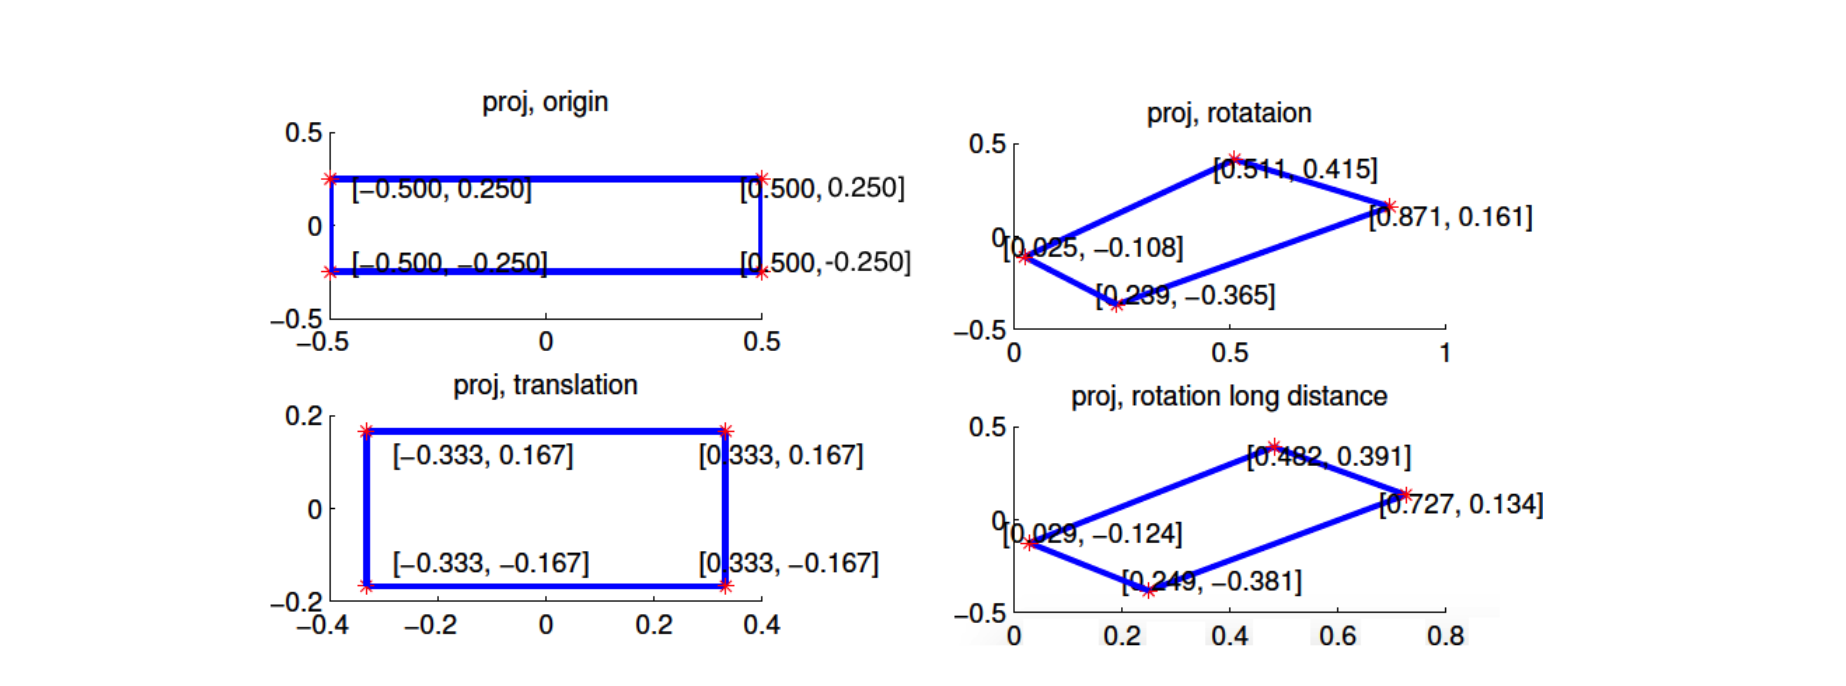
\includegraphics{new.png}
\caption{Sample Plots}
\end{figure}

\begin{enumerate}
\def\labelenumi{\arabic{enumi}.}
\tightlist
\item
  {[}No rigid body transformation{]}. Focal length = 1. The optical axis
  of the camera is aligned with the z-axis.
\item
  {[}Translation{]}. \(^BO_A = [\text{0 0 1}]^T\). Focal length = 1. The
  optical axis of the camera is aligned with the z-axis.
\item
  {[}Translation and Rotation{]}. Focal length = 1. \(^B_AR\) encodes a
  30 degrees around the z-axis and then 60 degrees around the y-axis.
  \(^BO_A = [\text{0 0 1}]^T\).
\item
  {[}Translation and Rotation, long distance{]}. Focal length = 5.
  \(^B_AR\) encodes a 30 degrees around the z-axis and then 60 degrees
  around the y-axis. \(^BO_A = [\text{0 0 13}]^T\).
\end{enumerate}

\begin{quote}
You can refer the Richard Szeliski starting page 36 for image formation
and the extrinsic matrix.
\end{quote}

\begin{quote}
Intrinsic matrix calculation for perspective camera models was covered
in class and can be referred in slide 2\\
https://cseweb.ucsd.edu/classes/fa19/cse252A-a/lec2.pdf\\
You can also refer lecture 3 of the previous year's course as well for
further information if you wish!\\
http://cseweb.ucsd.edu/classes/fa18/cse252A-a/lec3.pdf
\end{quote}

We will not use a full intrinsic camera matrix (e.g.~that maps
centimeters to pixels, and defines the coordinates of the center of the
image), but only parameterize this with \(f\), the focal length. In
other words: the only parameter in the intrinsic camera matrix under the
perspective assumption is \(f\).

    \begin{tcolorbox}[breakable, size=fbox, boxrule=1pt, pad at break*=1mm,colback=cellbackground, colframe=cellborder]
\prompt{In}{incolor}{11}{\boxspacing}
\begin{Verbatim}[commandchars=\\\{\}]
\PY{k+kn}{import} \PY{n+nn}{numpy} \PY{k}{as} \PY{n+nn}{np}
\PY{k+kn}{import} \PY{n+nn}{matplotlib}\PY{n+nn}{.}\PY{n+nn}{pyplot} \PY{k}{as} \PY{n+nn}{plt}
\PY{k+kn}{import} \PY{n+nn}{math}


\PY{c+c1}{\PYZsh{} convert points from euclidian to homogeneous}
\PY{k}{def} \PY{n+nf}{to\PYZus{}homog}\PY{p}{(}\PY{n}{points}\PY{p}{)}\PY{p}{:} \PY{c+c1}{\PYZsh{}here always remember that points is a 3x4 matrix}
    \PY{k}{return} \PY{n}{np}\PY{o}{.}\PY{n}{vstack}\PY{p}{(}\PY{p}{(}\PY{n}{points}\PY{p}{,} \PY{n}{points}\PY{p}{[}\PY{l+m+mi}{0}\PY{p}{]}\PY{o}{.}\PY{n}{size} \PY{o}{*} \PY{p}{[}\PY{l+m+mi}{1}\PY{p}{]}\PY{p}{)}\PY{p}{)}
    


\PY{c+c1}{\PYZsh{} convert points from homogeneous to euclidian}
\PY{k}{def} \PY{n+nf}{from\PYZus{}homog}\PY{p}{(}\PY{n}{points\PYZus{}homog}\PY{p}{)}\PY{p}{:}  
    \PY{k}{return}  \PY{n}{points\PYZus{}homog} \PY{o}{/} \PY{n}{points\PYZus{}homog}\PY{p}{[}\PY{o}{\PYZhy{}}\PY{l+m+mi}{1}\PY{p}{,}\PY{p}{:}\PY{p}{]}


\PY{c+c1}{\PYZsh{} project 3D euclidian points to 2D euclidian}
\PY{k}{def} \PY{n+nf}{project\PYZus{}points}\PY{p}{(}\PY{n}{P\PYZus{}int}\PY{p}{,} \PY{n}{P\PYZus{}ext}\PY{p}{,} \PY{n}{pts}\PY{p}{)}\PY{p}{:}
    \PY{n}{transformation} \PY{o}{=} \PY{n}{np}\PY{o}{.}\PY{n}{matmul}\PY{p}{(}\PY{n}{P\PYZus{}int}\PY{p}{,}\PY{n}{P\PYZus{}ext}\PY{p}{)}
    \PY{n}{pts\PYZus{}final} \PY{o}{=} \PY{n}{np}\PY{o}{.}\PY{n}{matmul}\PY{p}{(}\PY{n}{transformation}\PY{p}{,} \PY{n}{to\PYZus{}homog}\PY{p}{(}\PY{n}{pts}\PY{p}{)}\PY{p}{)}
    \PY{k}{return} \PY{n}{from\PYZus{}homog}\PY{p}{(}\PY{n}{pts\PYZus{}final}\PY{p}{)}
\end{Verbatim}
\end{tcolorbox}

    \begin{tcolorbox}[breakable, size=fbox, boxrule=1pt, pad at break*=1mm,colback=cellbackground, colframe=cellborder]
\prompt{In}{incolor}{12}{\boxspacing}
\begin{Verbatim}[commandchars=\\\{\}]
\PY{c+c1}{\PYZsh{} Change the three matrices for the four cases as described in the problem}
\PY{c+c1}{\PYZsh{} in the four camera functions geiven below. Make sure that we can see the formula}
\PY{c+c1}{\PYZsh{} (if one exists) being used to fill in the matrices. Feel free to document with}
\PY{c+c1}{\PYZsh{} comments any thing you feel the need to explain. }

\PY{k}{def} \PY{n+nf}{camera1}\PY{p}{(}\PY{p}{)}\PY{p}{:}
    \PY{n}{P\PYZus{}int\PYZus{}proj} \PY{o}{=} \PY{n}{np}\PY{o}{.}\PY{n}{array}\PY{p}{(}\PY{p}{[}\PY{p}{[}\PY{l+m+mi}{1}\PY{p}{,} \PY{l+m+mi}{0}\PY{p}{,} \PY{l+m+mi}{0}\PY{p}{,} \PY{l+m+mi}{0}\PY{p}{]}\PY{p}{,} \PY{p}{[}\PY{l+m+mi}{0}\PY{p}{,} \PY{l+m+mi}{1}\PY{p}{,} \PY{l+m+mi}{0}\PY{p}{,} \PY{l+m+mi}{0}\PY{p}{]}\PY{p}{,} \PY{p}{[}\PY{l+m+mi}{0}\PY{p}{,} \PY{l+m+mi}{0}\PY{p}{,} \PY{l+m+mi}{1}\PY{p}{,} \PY{l+m+mi}{0}\PY{p}{]}\PY{p}{]}\PY{p}{)}
    \PY{n}{P\PYZus{}ext} \PY{o}{=} \PY{n}{np}\PY{o}{.}\PY{n}{array}\PY{p}{(}\PY{p}{[}\PY{p}{[}\PY{l+m+mi}{1}\PY{p}{,} \PY{l+m+mi}{0}\PY{p}{,} \PY{l+m+mi}{0}\PY{p}{,} \PY{l+m+mi}{0}\PY{p}{]}\PY{p}{,} \PY{p}{[}\PY{l+m+mi}{0}\PY{p}{,} \PY{l+m+mi}{1}\PY{p}{,} \PY{l+m+mi}{0}\PY{p}{,} \PY{l+m+mi}{0}\PY{p}{]}\PY{p}{,} \PY{p}{[}\PY{l+m+mi}{0}\PY{p}{,} \PY{l+m+mi}{0}\PY{p}{,} \PY{l+m+mi}{1}\PY{p}{,} \PY{l+m+mi}{0}\PY{p}{]}\PY{p}{,} \PY{p}{[}\PY{l+m+mi}{0}\PY{p}{,} \PY{l+m+mi}{0}\PY{p}{,} \PY{l+m+mi}{0}\PY{p}{,} \PY{l+m+mi}{1}\PY{p}{]}\PY{p}{]}\PY{p}{)} \PY{c+c1}{\PYZsh{}4x4 identity matrix}
    
    \PY{k}{return} \PY{n}{P\PYZus{}int\PYZus{}proj}\PY{p}{,} \PY{n}{P\PYZus{}ext}

\PY{k}{def} \PY{n+nf}{camera2}\PY{p}{(}\PY{p}{)}\PY{p}{:}
    \PY{n}{P\PYZus{}int\PYZus{}proj} \PY{o}{=} \PY{n}{np}\PY{o}{.}\PY{n}{array}\PY{p}{(}\PY{p}{[}\PY{p}{[}\PY{l+m+mi}{1}\PY{p}{,} \PY{l+m+mi}{0}\PY{p}{,} \PY{l+m+mi}{0}\PY{p}{,} \PY{l+m+mi}{0}\PY{p}{]}\PY{p}{,} \PY{p}{[}\PY{l+m+mi}{0}\PY{p}{,} \PY{l+m+mi}{1}\PY{p}{,} \PY{l+m+mi}{0}\PY{p}{,} \PY{l+m+mi}{0}\PY{p}{]}\PY{p}{,} \PY{p}{[}\PY{l+m+mi}{0}\PY{p}{,} \PY{l+m+mi}{0}\PY{p}{,} \PY{l+m+mi}{1}\PY{p}{,} \PY{l+m+mi}{0}\PY{p}{]}\PY{p}{]}\PY{p}{)}
    \PY{n}{P\PYZus{}ext} \PY{o}{=} \PY{n}{np}\PY{o}{.}\PY{n}{array}\PY{p}{(}\PY{p}{[}\PY{p}{[}\PY{l+m+mi}{1}\PY{p}{,} \PY{l+m+mi}{0}\PY{p}{,} \PY{l+m+mi}{0}\PY{p}{,} \PY{l+m+mi}{0}\PY{p}{]}\PY{p}{,} \PY{p}{[}\PY{l+m+mi}{0}\PY{p}{,} \PY{l+m+mi}{1}\PY{p}{,} \PY{l+m+mi}{0}\PY{p}{,} \PY{l+m+mi}{0}\PY{p}{]}\PY{p}{,} \PY{p}{[}\PY{l+m+mi}{0}\PY{p}{,} \PY{l+m+mi}{0}\PY{p}{,} \PY{l+m+mi}{1}\PY{p}{,} \PY{l+m+mi}{1}\PY{p}{]}\PY{p}{,} \PY{p}{[}\PY{l+m+mi}{0}\PY{p}{,} \PY{l+m+mi}{0}\PY{p}{,} \PY{l+m+mi}{0}\PY{p}{,} \PY{l+m+mi}{1}\PY{p}{]}\PY{p}{]}\PY{p}{)} \PY{c+c1}{\PYZsh{}4x4 translation matrix}
    
    \PY{k}{return} \PY{n}{P\PYZus{}int\PYZus{}proj}\PY{p}{,} \PY{n}{P\PYZus{}ext}

\PY{k}{def} \PY{n+nf}{camera3}\PY{p}{(}\PY{p}{)}\PY{p}{:}
    \PY{n}{P\PYZus{}int\PYZus{}proj} \PY{o}{=} \PY{n}{np}\PY{o}{.}\PY{n}{array}\PY{p}{(}\PY{p}{[}\PY{p}{[}\PY{l+m+mi}{1}\PY{p}{,} \PY{l+m+mi}{0}\PY{p}{,} \PY{l+m+mi}{0}\PY{p}{,} \PY{l+m+mi}{0}\PY{p}{]}\PY{p}{,} \PY{p}{[}\PY{l+m+mi}{0}\PY{p}{,} \PY{l+m+mi}{1}\PY{p}{,} \PY{l+m+mi}{0}\PY{p}{,} \PY{l+m+mi}{0}\PY{p}{]}\PY{p}{,} \PY{p}{[}\PY{l+m+mi}{0}\PY{p}{,} \PY{l+m+mi}{0}\PY{p}{,} \PY{l+m+mi}{1}\PY{p}{,} \PY{l+m+mi}{0}\PY{p}{]}\PY{p}{]}\PY{p}{)}
    \PY{n}{rot\PYZus{}z} \PY{o}{=} \PY{n}{np}\PY{o}{.}\PY{n}{array}\PY{p}{(}\PY{p}{[}\PY{p}{[}\PY{n}{math}\PY{o}{.}\PY{n}{cos}\PY{p}{(}\PY{l+m+mi}{30}\PY{p}{)}\PY{p}{,} \PY{o}{\PYZhy{}}\PY{l+m+mi}{1}\PY{o}{*}\PY{n}{math}\PY{o}{.}\PY{n}{sin}\PY{p}{(}\PY{l+m+mi}{30}\PY{p}{)}\PY{p}{,} \PY{l+m+mi}{0}\PY{p}{,} \PY{l+m+mi}{0}\PY{p}{]}\PY{p}{,} 
                      \PY{p}{[}\PY{n}{math}\PY{o}{.}\PY{n}{sin}\PY{p}{(}\PY{l+m+mi}{30}\PY{p}{)}\PY{p}{,} \PY{n}{math}\PY{o}{.}\PY{n}{cos}\PY{p}{(}\PY{l+m+mi}{30}\PY{p}{)}\PY{p}{,} \PY{l+m+mi}{0}\PY{p}{,} \PY{l+m+mi}{0}\PY{p}{]}\PY{p}{,} 
                      \PY{p}{[}\PY{l+m+mi}{0}\PY{p}{,} \PY{l+m+mi}{0}\PY{p}{,} \PY{l+m+mi}{1}\PY{p}{,} \PY{l+m+mi}{0}\PY{p}{]}\PY{p}{,} \PY{p}{[}\PY{l+m+mi}{0}\PY{p}{,} \PY{l+m+mi}{0}\PY{p}{,} \PY{l+m+mi}{0}\PY{p}{,} \PY{l+m+mi}{1}\PY{p}{]}\PY{p}{]}\PY{p}{)}
    \PY{n}{rot\PYZus{}y} \PY{o}{=} \PY{n}{np}\PY{o}{.}\PY{n}{array}\PY{p}{(}\PY{p}{[}\PY{p}{[}\PY{n}{math}\PY{o}{.}\PY{n}{cos}\PY{p}{(}\PY{l+m+mi}{60}\PY{p}{)}\PY{p}{,} \PY{l+m+mi}{0}\PY{p}{,} \PY{n}{math}\PY{o}{.}\PY{n}{sin}\PY{p}{(}\PY{l+m+mi}{60}\PY{p}{)}\PY{p}{,} \PY{l+m+mi}{0}\PY{p}{]}\PY{p}{,} \PY{p}{[}\PY{l+m+mi}{0}\PY{p}{,} \PY{l+m+mi}{1}\PY{p}{,} \PY{l+m+mi}{0}\PY{p}{,} \PY{l+m+mi}{0}\PY{p}{]}\PY{p}{,}
                      \PY{p}{[}\PY{o}{\PYZhy{}}\PY{l+m+mi}{1}\PY{o}{*}\PY{n}{math}\PY{o}{.}\PY{n}{sin}\PY{p}{(}\PY{l+m+mi}{60}\PY{p}{)}\PY{p}{,} \PY{l+m+mi}{0}\PY{p}{,} \PY{n}{math}\PY{o}{.}\PY{n}{cos}\PY{p}{(}\PY{l+m+mi}{60}\PY{p}{)}\PY{p}{,} \PY{l+m+mi}{0}\PY{p}{]}\PY{p}{,} \PY{p}{[}\PY{l+m+mi}{0}\PY{p}{,} \PY{l+m+mi}{0}\PY{p}{,} \PY{l+m+mi}{0}\PY{p}{,} \PY{l+m+mi}{1}\PY{p}{]}\PY{p}{]}\PY{p}{)}
    \PY{n}{translation} \PY{o}{=} \PY{n}{np}\PY{o}{.}\PY{n}{array}\PY{p}{(}\PY{p}{[}\PY{p}{[}\PY{l+m+mi}{1}\PY{p}{,} \PY{l+m+mi}{0}\PY{p}{,} \PY{l+m+mi}{0}\PY{p}{,} \PY{l+m+mi}{0}\PY{p}{]}\PY{p}{,} \PY{p}{[}\PY{l+m+mi}{0}\PY{p}{,} \PY{l+m+mi}{1}\PY{p}{,} \PY{l+m+mi}{0}\PY{p}{,} \PY{l+m+mi}{0}\PY{p}{]}\PY{p}{,} \PY{p}{[}\PY{l+m+mi}{0}\PY{p}{,} \PY{l+m+mi}{0}\PY{p}{,} \PY{l+m+mi}{1}\PY{p}{,} \PY{l+m+mi}{1}\PY{p}{]}\PY{p}{,} \PY{p}{[}\PY{l+m+mi}{0}\PY{p}{,} \PY{l+m+mi}{0}\PY{p}{,} \PY{l+m+mi}{0}\PY{p}{,} \PY{l+m+mi}{1}\PY{p}{]}\PY{p}{]}\PY{p}{)}
    \PY{n}{rotation} \PY{o}{=} \PY{n}{np}\PY{o}{.}\PY{n}{matmul}\PY{p}{(}\PY{n}{rot\PYZus{}y}\PY{p}{,}\PY{n}{rot\PYZus{}z}\PY{p}{)}
    \PY{n}{P\PYZus{}ext} \PY{o}{=} \PY{n}{np}\PY{o}{.}\PY{n}{matmul}\PY{p}{(}\PY{n}{rotation}\PY{p}{,} \PY{n}{translation}\PY{p}{)}

    \PY{k}{return} \PY{n}{P\PYZus{}int\PYZus{}proj}\PY{p}{,} \PY{n}{P\PYZus{}ext}

\PY{k}{def} \PY{n+nf}{camera4}\PY{p}{(}\PY{p}{)}\PY{p}{:}    
    \PY{n}{P\PYZus{}int\PYZus{}proj} \PY{o}{=} \PY{n}{np}\PY{o}{.}\PY{n}{array}\PY{p}{(}\PY{p}{[}\PY{p}{[}\PY{l+m+mi}{1}\PY{p}{,} \PY{l+m+mi}{0}\PY{p}{,} \PY{l+m+mi}{0}\PY{p}{,} \PY{l+m+mi}{0}\PY{p}{]}\PY{p}{,} \PY{p}{[}\PY{l+m+mi}{0}\PY{p}{,} \PY{l+m+mi}{1}\PY{p}{,} \PY{l+m+mi}{0}\PY{p}{,} \PY{l+m+mi}{0}\PY{p}{]}\PY{p}{,} \PY{p}{[}\PY{l+m+mi}{0}\PY{p}{,} \PY{l+m+mi}{0}\PY{p}{,} \PY{l+m+mi}{1}\PY{o}{/}\PY{l+m+mi}{5}\PY{p}{,} \PY{l+m+mi}{0}\PY{p}{]}\PY{p}{]}\PY{p}{)}
    \PY{n}{rot\PYZus{}z} \PY{o}{=} \PY{n}{np}\PY{o}{.}\PY{n}{array}\PY{p}{(}\PY{p}{[}\PY{p}{[}\PY{n}{math}\PY{o}{.}\PY{n}{cos}\PY{p}{(}\PY{n}{math}\PY{o}{.}\PY{n}{radians}\PY{p}{(}\PY{l+m+mi}{30}\PY{p}{)}\PY{p}{)}\PY{p}{,} \PY{o}{\PYZhy{}}\PY{l+m+mi}{1}\PY{o}{*}\PY{n}{math}\PY{o}{.}\PY{n}{sin}\PY{p}{(}\PY{n}{math}\PY{o}{.}\PY{n}{radians}\PY{p}{(}\PY{l+m+mi}{30}\PY{p}{)}\PY{p}{)}\PY{p}{,} \PY{l+m+mi}{0}\PY{p}{,} \PY{l+m+mi}{0}\PY{p}{]}\PY{p}{,} 
                      \PY{p}{[}\PY{n}{math}\PY{o}{.}\PY{n}{sin}\PY{p}{(}\PY{n}{math}\PY{o}{.}\PY{n}{radians}\PY{p}{(}\PY{l+m+mi}{30}\PY{p}{)}\PY{p}{)}\PY{p}{,} \PY{n}{math}\PY{o}{.}\PY{n}{cos}\PY{p}{(}\PY{n}{math}\PY{o}{.}\PY{n}{radians}\PY{p}{(}\PY{l+m+mi}{30}\PY{p}{)}\PY{p}{)}\PY{p}{,} \PY{l+m+mi}{0}\PY{p}{,} \PY{l+m+mi}{0}\PY{p}{]}\PY{p}{,} 
                      \PY{p}{[}\PY{l+m+mi}{0}\PY{p}{,} \PY{l+m+mi}{0}\PY{p}{,} \PY{l+m+mi}{1}\PY{p}{,} \PY{l+m+mi}{0}\PY{p}{]}\PY{p}{,} \PY{p}{[}\PY{l+m+mi}{0}\PY{p}{,} \PY{l+m+mi}{0}\PY{p}{,} \PY{l+m+mi}{0}\PY{p}{,} \PY{l+m+mi}{1}\PY{p}{]}\PY{p}{]}\PY{p}{)}
    \PY{n}{rot\PYZus{}y} \PY{o}{=} \PY{n}{np}\PY{o}{.}\PY{n}{array}\PY{p}{(}\PY{p}{[}\PY{p}{[}\PY{n}{math}\PY{o}{.}\PY{n}{cos}\PY{p}{(}\PY{n}{math}\PY{o}{.}\PY{n}{radians}\PY{p}{(}\PY{l+m+mi}{60}\PY{p}{)}\PY{p}{)}\PY{p}{,} \PY{l+m+mi}{0}\PY{p}{,} \PY{n}{math}\PY{o}{.}\PY{n}{sin}\PY{p}{(}\PY{n}{math}\PY{o}{.}\PY{n}{radians}\PY{p}{(}\PY{l+m+mi}{60}\PY{p}{)}\PY{p}{)}\PY{p}{,} \PY{l+m+mi}{0}\PY{p}{]}\PY{p}{,} \PY{p}{[}\PY{l+m+mi}{0}\PY{p}{,} \PY{l+m+mi}{1}\PY{p}{,} \PY{l+m+mi}{0}\PY{p}{,} \PY{l+m+mi}{0}\PY{p}{]}\PY{p}{,}
                      \PY{p}{[}\PY{o}{\PYZhy{}}\PY{l+m+mi}{1}\PY{o}{*}\PY{n}{math}\PY{o}{.}\PY{n}{sin}\PY{p}{(}\PY{n}{math}\PY{o}{.}\PY{n}{radians}\PY{p}{(}\PY{l+m+mi}{60}\PY{p}{)}\PY{p}{)}\PY{p}{,} \PY{l+m+mi}{0}\PY{p}{,} \PY{n}{math}\PY{o}{.}\PY{n}{cos}\PY{p}{(}\PY{n}{math}\PY{o}{.}\PY{n}{radians}\PY{p}{(}\PY{l+m+mi}{60}\PY{p}{)}\PY{p}{)}\PY{p}{,} \PY{l+m+mi}{0}\PY{p}{]}\PY{p}{,} \PY{p}{[}\PY{l+m+mi}{0}\PY{p}{,} \PY{l+m+mi}{0}\PY{p}{,} \PY{l+m+mi}{0}\PY{p}{,} \PY{l+m+mi}{1}\PY{p}{]}\PY{p}{]}\PY{p}{)}
    \PY{n}{translation} \PY{o}{=} \PY{n}{np}\PY{o}{.}\PY{n}{array}\PY{p}{(}\PY{p}{[}\PY{p}{[}\PY{l+m+mi}{1}\PY{p}{,} \PY{l+m+mi}{0}\PY{p}{,} \PY{l+m+mi}{0}\PY{p}{,} \PY{l+m+mi}{0}\PY{p}{]}\PY{p}{,} \PY{p}{[}\PY{l+m+mi}{0}\PY{p}{,} \PY{l+m+mi}{1}\PY{p}{,} \PY{l+m+mi}{0}\PY{p}{,} \PY{l+m+mi}{0}\PY{p}{]}\PY{p}{,} \PY{p}{[}\PY{l+m+mi}{0}\PY{p}{,} \PY{l+m+mi}{0}\PY{p}{,} \PY{l+m+mi}{1}\PY{p}{,} \PY{l+m+mi}{13}\PY{p}{]}\PY{p}{,} \PY{p}{[}\PY{l+m+mi}{0}\PY{p}{,} \PY{l+m+mi}{0}\PY{p}{,} \PY{l+m+mi}{0}\PY{p}{,} \PY{l+m+mi}{1}\PY{p}{]}\PY{p}{]}\PY{p}{)}
    \PY{n}{rotation} \PY{o}{=} \PY{n}{np}\PY{o}{.}\PY{n}{matmul}\PY{p}{(}\PY{n}{rot\PYZus{}y}\PY{p}{,}\PY{n}{rot\PYZus{}z}\PY{p}{)}
    \PY{n}{P\PYZus{}ext} \PY{o}{=} \PY{n}{np}\PY{o}{.}\PY{n}{matmul}\PY{p}{(}\PY{n}{translation}\PY{p}{,}\PY{n}{rotation}\PY{p}{)}
    \PY{k}{return} \PY{n}{P\PYZus{}int\PYZus{}proj}\PY{p}{,} \PY{n}{P\PYZus{}ext}

\PY{c+c1}{\PYZsh{} Use the following code to display your outputs}
\PY{c+c1}{\PYZsh{} You are free to change the axis parameters to better }
\PY{c+c1}{\PYZsh{} display your quadrilateral but do not remove any annotations}

\PY{k}{def} \PY{n+nf}{plot\PYZus{}points}\PY{p}{(}\PY{n}{points}\PY{p}{,} \PY{n}{title}\PY{o}{=}\PY{l+s+s1}{\PYZsq{}}\PY{l+s+s1}{\PYZsq{}}\PY{p}{,} \PY{n}{style}\PY{o}{=}\PY{l+s+s1}{\PYZsq{}}\PY{l+s+s1}{.\PYZhy{}r}\PY{l+s+s1}{\PYZsq{}}\PY{p}{,} \PY{n}{axis}\PY{o}{=}\PY{p}{[}\PY{p}{]}\PY{p}{)}\PY{p}{:}
    \PY{n}{inds} \PY{o}{=} \PY{n+nb}{list}\PY{p}{(}\PY{n+nb}{range}\PY{p}{(}\PY{n}{points}\PY{o}{.}\PY{n}{shape}\PY{p}{[}\PY{l+m+mi}{1}\PY{p}{]}\PY{p}{)}\PY{p}{)}\PY{o}{+}\PY{p}{[}\PY{l+m+mi}{0}\PY{p}{]}
    \PY{n}{plt}\PY{o}{.}\PY{n}{plot}\PY{p}{(}\PY{n}{points}\PY{p}{[}\PY{l+m+mi}{0}\PY{p}{,}\PY{n}{inds}\PY{p}{]}\PY{p}{,} \PY{n}{points}\PY{p}{[}\PY{l+m+mi}{1}\PY{p}{,}\PY{n}{inds}\PY{p}{]}\PY{p}{,}\PY{n}{style}\PY{p}{)}
    
    \PY{k}{for} \PY{n}{i} \PY{o+ow}{in} \PY{n+nb}{range}\PY{p}{(}\PY{n+nb}{len}\PY{p}{(}\PY{n}{points}\PY{p}{[}\PY{l+m+mi}{0}\PY{p}{,}\PY{n}{inds}\PY{p}{]}\PY{p}{)}\PY{p}{)}\PY{p}{:}
        \PY{n}{plt}\PY{o}{.}\PY{n}{annotate}\PY{p}{(}\PY{n+nb}{str}\PY{p}{(}\PY{l+s+s2}{\PYZdq{}}\PY{l+s+si}{\PYZob{}0:.3f\PYZcb{}}\PY{l+s+s2}{\PYZdq{}}\PY{o}{.}\PY{n}{format}\PY{p}{(}\PY{n}{points}\PY{p}{[}\PY{l+m+mi}{0}\PY{p}{,}\PY{n}{inds}\PY{p}{]}\PY{p}{[}\PY{n}{i}\PY{p}{]}\PY{p}{)}\PY{p}{)}\PY{o}{+}\PY{l+s+s2}{\PYZdq{}}\PY{l+s+s2}{,}\PY{l+s+s2}{\PYZdq{}}\PY{o}{+}\PY{n+nb}{str}\PY{p}{(}\PY{l+s+s2}{\PYZdq{}}\PY{l+s+si}{\PYZob{}0:.3f\PYZcb{}}\PY{l+s+s2}{\PYZdq{}}\PY{o}{.}\PY{n}{format}\PY{p}{(}\PY{n}{points}\PY{p}{[}\PY{l+m+mi}{1}\PY{p}{,}\PY{n}{inds}\PY{p}{]}\PY{p}{[}\PY{n}{i}\PY{p}{]}\PY{p}{)}\PY{p}{)}\PY{p}{,}\PY{p}{(}\PY{n}{points}\PY{p}{[}\PY{l+m+mi}{0}\PY{p}{,}\PY{n}{inds}\PY{p}{]}\PY{p}{[}\PY{n}{i}\PY{p}{]}\PY{p}{,} \PY{n}{points}\PY{p}{[}\PY{l+m+mi}{1}\PY{p}{,}\PY{n}{inds}\PY{p}{]}\PY{p}{[}\PY{n}{i}\PY{p}{]}\PY{p}{)}\PY{p}{)}
    
    \PY{k}{if} \PY{n}{title}\PY{p}{:}
        \PY{n}{plt}\PY{o}{.}\PY{n}{title}\PY{p}{(}\PY{n}{title}\PY{p}{)}
    \PY{k}{if} \PY{n}{axis}\PY{p}{:}
        \PY{n}{plt}\PY{o}{.}\PY{n}{axis}\PY{p}{(}\PY{n}{axis}\PY{p}{)}
        
    \PY{n}{plt}\PY{o}{.}\PY{n}{tight\PYZus{}layout}\PY{p}{(}\PY{p}{)}
        
\PY{k}{def} \PY{n+nf}{main}\PY{p}{(}\PY{p}{)}\PY{p}{:}
    \PY{n}{point1} \PY{o}{=} \PY{n}{np}\PY{o}{.}\PY{n}{array}\PY{p}{(}\PY{p}{[}\PY{p}{[}\PY{o}{\PYZhy{}}\PY{l+m+mi}{1}\PY{p}{,}\PY{o}{\PYZhy{}}\PY{o}{.}\PY{l+m+mi}{5}\PY{p}{,}\PY{l+m+mi}{2}\PY{p}{]}\PY{p}{]}\PY{p}{)}\PY{o}{.}\PY{n}{T}
    \PY{n}{point2} \PY{o}{=} \PY{n}{np}\PY{o}{.}\PY{n}{array}\PY{p}{(}\PY{p}{[}\PY{p}{[}\PY{l+m+mi}{1}\PY{p}{,}\PY{o}{\PYZhy{}}\PY{o}{.}\PY{l+m+mi}{5}\PY{p}{,}\PY{l+m+mi}{2}\PY{p}{]}\PY{p}{]}\PY{p}{)}\PY{o}{.}\PY{n}{T}
    \PY{n}{point3} \PY{o}{=} \PY{n}{np}\PY{o}{.}\PY{n}{array}\PY{p}{(}\PY{p}{[}\PY{p}{[}\PY{l+m+mi}{1}\PY{p}{,}\PY{o}{.}\PY{l+m+mi}{5}\PY{p}{,}\PY{l+m+mi}{2}\PY{p}{]}\PY{p}{]}\PY{p}{)}\PY{o}{.}\PY{n}{T}
    \PY{n}{point4} \PY{o}{=} \PY{n}{np}\PY{o}{.}\PY{n}{array}\PY{p}{(}\PY{p}{[}\PY{p}{[}\PY{o}{\PYZhy{}}\PY{l+m+mi}{1}\PY{p}{,}\PY{o}{.}\PY{l+m+mi}{5}\PY{p}{,}\PY{l+m+mi}{2}\PY{p}{]}\PY{p}{]}\PY{p}{)}\PY{o}{.}\PY{n}{T} 
    \PY{n}{points} \PY{o}{=} \PY{n}{np}\PY{o}{.}\PY{n}{hstack}\PY{p}{(}\PY{p}{(}\PY{n}{point1}\PY{p}{,}\PY{n}{point2}\PY{p}{,}\PY{n}{point3}\PY{p}{,}\PY{n}{point4}\PY{p}{)}\PY{p}{)}
    
    \PY{k}{for} \PY{n}{i}\PY{p}{,} \PY{n}{camera} \PY{o+ow}{in} \PY{n+nb}{enumerate}\PY{p}{(}\PY{p}{[}\PY{n}{camera1}\PY{p}{,} \PY{n}{camera2}\PY{p}{,} \PY{n}{camera3}\PY{p}{,} \PY{n}{camera4}\PY{p}{]}\PY{p}{)}\PY{p}{:}
        \PY{n}{P\PYZus{}int\PYZus{}proj}\PY{p}{,} \PY{n}{P\PYZus{}ext} \PY{o}{=} \PY{n}{camera}\PY{p}{(}\PY{p}{)}
        \PY{n}{plt}\PY{o}{.}\PY{n}{subplot}\PY{p}{(}\PY{l+m+mi}{2}\PY{p}{,} \PY{l+m+mi}{2}\PY{p}{,} \PY{n}{i}\PY{o}{+}\PY{l+m+mi}{1}\PY{p}{)}
        \PY{n}{plot\PYZus{}points}\PY{p}{(}\PY{n}{project\PYZus{}points}\PY{p}{(}\PY{n}{P\PYZus{}int\PYZus{}proj}\PY{p}{,} \PY{n}{P\PYZus{}ext}\PY{p}{,} \PY{n}{points}\PY{p}{)}\PY{p}{,} \PY{n}{title}\PY{o}{=}\PY{l+s+s1}{\PYZsq{}}\PY{l+s+s1}{Camera }\PY{l+s+si}{\PYZpc{}d}\PY{l+s+s1}{ Projective}\PY{l+s+s1}{\PYZsq{}}\PY{o}{\PYZpc{}}\PY{p}{(}\PY{n}{i}\PY{o}{+}\PY{l+m+mi}{1}\PY{p}{)}\PY{p}{,} \PY{n}{axis}\PY{o}{=}\PY{p}{[}\PY{o}{\PYZhy{}}\PY{l+m+mf}{0.6}\PY{p}{,}\PY{l+m+mi}{1}\PY{p}{,}\PY{o}{\PYZhy{}}\PY{l+m+mf}{0.75}\PY{p}{,}\PY{l+m+mf}{0.75}\PY{p}{]}\PY{p}{)}
        \PY{n}{plt}\PY{o}{.}\PY{n}{show}\PY{p}{(}\PY{p}{)}

\PY{n}{main}\PY{p}{(}\PY{p}{)}
\end{Verbatim}
\end{tcolorbox}

    \begin{center}
    \adjustimage{max size={0.9\linewidth}{0.9\paperheight}}{output_4_0.png}
    \end{center}
    { \hspace*{\fill} \\}
    
    \begin{center}
    \adjustimage{max size={0.9\linewidth}{0.9\paperheight}}{output_4_1.png}
    \end{center}
    { \hspace*{\fill} \\}
    
    \begin{center}
    \adjustimage{max size={0.9\linewidth}{0.9\paperheight}}{output_4_2.png}
    \end{center}
    { \hspace*{\fill} \\}
    
    \begin{center}
    \adjustimage{max size={0.9\linewidth}{0.9\paperheight}}{output_4_3.png}
    \end{center}
    { \hspace*{\fill} \\}
    
    \hypertarget{problem-3-homography-12-pts}{%
\subsection{Problem 3: Homography {[}12
pts{]}}\label{problem-3-homography-12-pts}}

Consider a vision application in which components of the scene are
replaced by components from another image scene.

In this problem, we will implement partial functionality of a smartphone
camera scanning application (Example: CamScanner) that, in case you've
never used before, takes pictures of documents and transforms it by
warping and aligning to give an image similar to one which would've been
obtained through using a scanner.

The transformation can be visualized by imagining the use of two cameras
forming an image of a scene with a document. The scene would be the
document you're trying to scan placed on a table and one of the cameras
would be your smart phone camera, forming the image that you'll be
uploading and using in this assignment. There can also be an ideally
placed camera, oriented in the world in such a way that the image it
forms of the scene has the document perfectly algined. While it is
unlikely you can hold your phone still enough to get such an image, we
can use homography to transform the image you take into the image that
the ideally placed camera would have taken.

This digital replacement is accomplished by a set of corresponding
points for the document in both the source (your picture) and target
(the ideal) images. The task then consists of mapping the points from
the source to their respective points in the target image. In the most
general case, there would be no constraints on the scene geometry,
making the problem quite hard to solve. If, however, the scene can be
approximated by a plane in 3D, a solution can be formulated much more
easily even without the knowledge of camera calibration parameters.

To solve this section of the homework, you will begin by understanding
the transformation that maps one image onto another in the planar scene
case. Then you will write a program that implements this transformation
and use it to warp some document into a well aligned document (See the
given example to understand what we mean by well aligned).

To begin with, we consider the projection of planes in images. imagine
two cameras \(C_1\) and \(C_2\) looking at a plane \(\pi\) in the world.
Consider a point \(P\) on the plane \(\pi\) and its projection
\(p=[\text{u1, v1, 1}]^T\) in the image 1 and \(q=[\text{u2, v2, 1}]^T\)
in image 2.

There exists a unique, upto scale, 3 \(\times\) 3 matrix \(H\) such
that, for any point \(P\): \[q \approx Hp\] Here \(\approx\) denotes
equality in homogeneous coordinates, meaning that the left and right
hand sides are proportional. Note that \(H\) only depends on the plane
and the projection matrices of the two cameras.

The interesting thing about this result is that by using \(H\) we can
compute the image of \(P\) that would be seen in the camera with center
\(C_2\) from the image of the point in the camera with center at
\(C_1\), without knowing the three dimensional location. Such an \(H\)
is a projective transformation of the plane, called a homography.

In this problem, complete the code for computeH and warp functions that
can be used in the skeletal code that follows.

There are three warp functions to implement in this assignment, example
ouputs of which are shown below. In warp1, you will create a homography
from points in your image to the target image (Mapping source points to
target points). In warp2, the inverse of this process will be done. In
warp3, you will create a homography between a given image and your
image, replacing your document with the given image.

\begin{enumerate}
\def\labelenumi{\arabic{enumi}.}
\item
  \begin{figure}
  \centering
  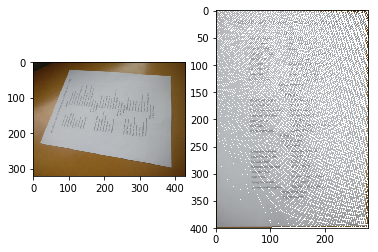
\includegraphics{forward.png}
  \caption{title}
  \end{figure}
\item
  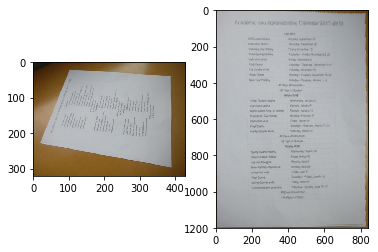
\includegraphics{inverse.png}\\
\item
  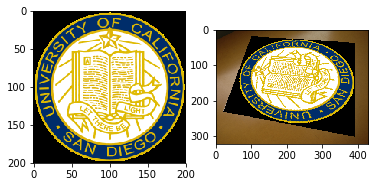
\includegraphics{backward.png}
\item
  In the context of this problem, the source image refers to the image
  of a document you take that needs to be replaced into the target.
\item
  The target image can start out as an empty matrix that you fill out
  using your code.
\item
  You will have to implement the computeH function that computes a
  homography. It takes in exactly four point correspondences between the
  source image and target image in homogeneous coordinates respectively
  and returns a 3 \(\times\) 3 homography matrix.
\item
  You will also have to implement the three warp functions in the
  skeleton code given and plot the resultant image pairs. For plotting,
  make sure that the target image is not smaller than the source image.
\end{enumerate}

Note: We have provided test code to check if your implementation for
computeH is correct. All the code to plot the results needed is also
provided along with the code to read in the images and other data
required for this problem. Please try not to modify that code.

You may find following python built-ins helpful: numpy.linalg.svd,
numpy.meshgrid

    \begin{tcolorbox}[breakable, size=fbox, boxrule=1pt, pad at break*=1mm,colback=cellbackground, colframe=cellborder]
\prompt{In}{incolor}{13}{\boxspacing}
\begin{Verbatim}[commandchars=\\\{\}]
\PY{k+kn}{import} \PY{n+nn}{numpy} \PY{k}{as} \PY{n+nn}{np}
\PY{k+kn}{from} \PY{n+nn}{PIL} \PY{k}{import} \PY{n}{Image}
\PY{k+kn}{import} \PY{n+nn}{matplotlib}\PY{n+nn}{.}\PY{n+nn}{pyplot} \PY{k}{as} \PY{n+nn}{plt}

\PY{c+c1}{\PYZsh{} load image to be used \PYZhy{} resize to make sure it\PYZsq{}s not too large}
\PY{c+c1}{\PYZsh{} You can use the given image as well}
\PY{c+c1}{\PYZsh{} A large image will make testing you code take longer; once you\PYZsq{}re satisfied with your result,}
\PY{c+c1}{\PYZsh{} you can, if you wish to, make the image larger (or till your computer memory allows you to)}

\PY{n}{source\PYZus{}image} \PY{o}{=} \PY{n}{np}\PY{o}{.}\PY{n}{array}\PY{p}{(}\PY{n}{Image}\PY{o}{.}\PY{n}{open}\PY{p}{(}\PY{l+s+s2}{\PYZdq{}}\PY{l+s+s2}{photo.jpg}\PY{l+s+s2}{\PYZdq{}}\PY{p}{)}\PY{p}{)}\PY{o}{/}\PY{l+m+mi}{255}

\PY{c+c1}{\PYZsh{} display images}
\PY{n}{plt}\PY{o}{.}\PY{n}{imshow}\PY{p}{(}\PY{n}{source\PYZus{}image}\PY{p}{)}

\PY{c+c1}{\PYZsh{} Align the polygon such that the corners align with the document in your picture}
\PY{c+c1}{\PYZsh{} This polygon doesn\PYZsq{}t need to overlap with the edges perfectly, an approximation is fine}
\PY{c+c1}{\PYZsh{} The order of points is clockwise, starting from bottom left.}
\PY{n}{x\PYZus{}coords} \PY{o}{=} \PY{p}{[}\PY{l+m+mi}{100}\PY{p}{,}\PY{l+m+mi}{500}\PY{p}{,}\PY{l+m+mi}{1950}\PY{p}{,}\PY{l+m+mi}{1950}\PY{p}{]} 
\PY{n}{y\PYZus{}coords} \PY{o}{=} \PY{p}{[}\PY{l+m+mi}{1170}\PY{p}{,}\PY{l+m+mi}{120}\PY{p}{,}\PY{l+m+mi}{210}\PY{p}{,}\PY{l+m+mi}{1500}\PY{p}{]}
\PY{n}{source\PYZus{}points} \PY{o}{=} \PY{n}{np}\PY{o}{.}\PY{n}{vstack}\PY{p}{(}\PY{p}{(}\PY{n}{x\PYZus{}coords}\PY{p}{,} \PY{n}{y\PYZus{}coords}\PY{p}{)}\PY{p}{)}

\PY{n}{plot\PYZus{}points}\PY{p}{(}\PY{n}{source\PYZus{}points}\PY{p}{)}

\PY{n}{plt}\PY{o}{.}\PY{n}{show}\PY{p}{(}\PY{p}{)}
\PY{n+nb}{print} \PY{p}{(}\PY{n}{source\PYZus{}image}\PY{o}{.}\PY{n}{shape}\PY{p}{)}
\end{Verbatim}
\end{tcolorbox}

    \begin{center}
    \adjustimage{max size={0.9\linewidth}{0.9\paperheight}}{output_6_0.png}
    \end{center}
    { \hspace*{\fill} \\}
    
    \begin{Verbatim}[commandchars=\\\{\}]
(1611, 2148, 3)
    \end{Verbatim}

    \begin{tcolorbox}[breakable, size=fbox, boxrule=1pt, pad at break*=1mm,colback=cellbackground, colframe=cellborder]
\prompt{In}{incolor}{14}{\boxspacing}
\begin{Verbatim}[commandchars=\\\{\}]
\PY{k}{def} \PY{n+nf}{computeH}\PY{p}{(}\PY{n}{source\PYZus{}points}\PY{p}{,} \PY{n}{target\PYZus{}points}\PY{p}{)}\PY{p}{:}
    \PY{c+c1}{\PYZsh{} returns the 3x3 homography matrix such that:}
    \PY{c+c1}{\PYZsh{} np.matmul(H, source\PYZus{}points) = target\PYZus{}points}
    \PY{c+c1}{\PYZsh{} where source\PYZus{}points and target\PYZus{}points are expected to be in homogeneous}
    \PY{c+c1}{\PYZsh{} make sure points are 3D homogeneous}
    \PY{k}{assert} \PY{n}{source\PYZus{}points}\PY{o}{.}\PY{n}{shape}\PY{p}{[}\PY{l+m+mi}{0}\PY{p}{]}\PY{o}{==}\PY{l+m+mi}{3} \PY{o+ow}{and} \PY{n}{target\PYZus{}points}\PY{o}{.}\PY{n}{shape}\PY{p}{[}\PY{l+m+mi}{0}\PY{p}{]}\PY{o}{==}\PY{l+m+mi}{3}
    \PY{c+c1}{\PYZsh{}compute H\PYZca{}\PYZhy{}1}
    \PY{n}{source\PYZus{}x1x2x3} \PY{o}{=} \PY{n}{source\PYZus{}points}\PY{p}{[}\PY{p}{:}\PY{p}{,}\PY{p}{:}\PY{l+m+mi}{3}\PY{p}{]}
    \PY{n}{source\PYZus{}x4} \PY{o}{=} \PY{n}{source\PYZus{}points}\PY{p}{[}\PY{p}{:}\PY{p}{,}\PY{o}{\PYZhy{}}\PY{l+m+mi}{1}\PY{p}{:}\PY{p}{]}
    \PY{n}{source\PYZus{}x1x2x3\PYZus{}inv} \PY{o}{=} \PY{n}{np}\PY{o}{.}\PY{n}{linalg}\PY{o}{.}\PY{n}{inv}\PY{p}{(}\PY{n}{source\PYZus{}x1x2x3}\PY{p}{)}
    \PY{n}{source\PYZus{}lambdas} \PY{o}{=} \PY{n}{np}\PY{o}{.}\PY{n}{matmul}\PY{p}{(}\PY{n}{source\PYZus{}x1x2x3\PYZus{}inv}\PY{p}{,}\PY{n}{source\PYZus{}x4}\PY{p}{)}
    \PY{n}{diag\PYZus{}source\PYZus{}lambdas} \PY{o}{=} \PY{n}{np}\PY{o}{.}\PY{n}{array}\PY{p}{(}\PY{p}{[}\PY{p}{[}\PY{n}{source\PYZus{}lambdas}\PY{p}{[}\PY{l+m+mi}{0}\PY{p}{,}\PY{l+m+mi}{0}\PY{p}{]}\PY{p}{,} \PY{l+m+mi}{0}\PY{p}{,} \PY{l+m+mi}{0}\PY{p}{]}\PY{p}{,} \PY{p}{[}\PY{l+m+mi}{0}\PY{p}{,} \PY{n}{source\PYZus{}lambdas}\PY{p}{[}\PY{l+m+mi}{1}\PY{p}{,}\PY{l+m+mi}{0}\PY{p}{]}\PY{p}{,} \PY{l+m+mi}{0}\PY{p}{]}\PY{p}{,} \PY{p}{[}\PY{l+m+mi}{0}\PY{p}{,} \PY{l+m+mi}{0}\PY{p}{,} \PY{n}{source\PYZus{}lambdas}\PY{p}{[}\PY{l+m+mi}{2}\PY{p}{,}\PY{l+m+mi}{0}\PY{p}{]}\PY{p}{]}\PY{p}{]}\PY{p}{)}
    \PY{n}{H\PYZus{}inv1} \PY{o}{=} \PY{n}{np}\PY{o}{.}\PY{n}{matmul}\PY{p}{(}\PY{n}{source\PYZus{}x1x2x3}\PY{p}{,}\PY{n}{diag\PYZus{}source\PYZus{}lambdas}\PY{p}{)}
    \PY{c+c1}{\PYZsh{}computer H\PYZca{}\PYZhy{}2}
    \PY{n}{target\PYZus{}x1x2x3} \PY{o}{=} \PY{n}{target\PYZus{}points}\PY{p}{[}\PY{p}{:}\PY{p}{,}\PY{p}{:}\PY{l+m+mi}{3}\PY{p}{]}
    \PY{n}{target\PYZus{}x4} \PY{o}{=} \PY{n}{target\PYZus{}points}\PY{p}{[}\PY{p}{:}\PY{p}{,}\PY{o}{\PYZhy{}}\PY{l+m+mi}{1}\PY{p}{:}\PY{p}{]}
    \PY{n}{target\PYZus{}x1x2x3\PYZus{}inv} \PY{o}{=} \PY{n}{np}\PY{o}{.}\PY{n}{linalg}\PY{o}{.}\PY{n}{inv}\PY{p}{(}\PY{n}{target\PYZus{}x1x2x3}\PY{p}{)}
    \PY{n}{target\PYZus{}lambdas} \PY{o}{=} \PY{n}{np}\PY{o}{.}\PY{n}{matmul}\PY{p}{(}\PY{n}{target\PYZus{}x1x2x3\PYZus{}inv}\PY{p}{,}\PY{n}{target\PYZus{}x4}\PY{p}{)}
    \PY{n}{diag\PYZus{}target\PYZus{}lambdas} \PY{o}{=} \PY{n}{np}\PY{o}{.}\PY{n}{array}\PY{p}{(}\PY{p}{[}\PY{p}{[}\PY{n}{target\PYZus{}lambdas}\PY{p}{[}\PY{l+m+mi}{0}\PY{p}{,}\PY{l+m+mi}{0}\PY{p}{]}\PY{p}{,} \PY{l+m+mi}{0}\PY{p}{,} \PY{l+m+mi}{0}\PY{p}{]}\PY{p}{,} \PY{p}{[}\PY{l+m+mi}{0}\PY{p}{,} \PY{n}{target\PYZus{}lambdas}\PY{p}{[}\PY{l+m+mi}{1}\PY{p}{,}\PY{l+m+mi}{0}\PY{p}{]}\PY{p}{,} \PY{l+m+mi}{0}\PY{p}{]}\PY{p}{,} \PY{p}{[}\PY{l+m+mi}{0}\PY{p}{,} \PY{l+m+mi}{0}\PY{p}{,} \PY{n}{target\PYZus{}lambdas}\PY{p}{[}\PY{l+m+mi}{2}\PY{p}{,}\PY{l+m+mi}{0}\PY{p}{]}\PY{p}{]}\PY{p}{]}\PY{p}{)}
    \PY{n}{H\PYZus{}inv2} \PY{o}{=} \PY{n}{np}\PY{o}{.}\PY{n}{matmul}\PY{p}{(}\PY{n}{target\PYZus{}x1x2x3}\PY{p}{,}\PY{n}{diag\PYZus{}target\PYZus{}lambdas}\PY{p}{)}
    
    \PY{n}{H\PYZus{}mtx} \PY{o}{=} \PY{n}{np}\PY{o}{.}\PY{n}{matmul}\PY{p}{(}\PY{n}{H\PYZus{}inv2}\PY{p}{,}\PY{n}{np}\PY{o}{.}\PY{n}{linalg}\PY{o}{.}\PY{n}{inv}\PY{p}{(}\PY{n}{H\PYZus{}inv1}\PY{p}{)}\PY{p}{)}

    \PY{k}{return}  \PY{n}{H\PYZus{}mtx}
\PY{c+c1}{\PYZsh{}\PYZsh{}\PYZsh{}\PYZsh{}\PYZsh{}\PYZsh{}\PYZsh{}\PYZsh{}\PYZsh{}\PYZsh{}\PYZsh{}\PYZsh{}\PYZsh{}\PYZsh{}\PYZsh{}\PYZsh{}\PYZsh{}\PYZsh{}\PYZsh{}\PYZsh{}\PYZsh{}\PYZsh{}\PYZsh{}\PYZsh{}\PYZsh{}\PYZsh{}\PYZsh{}\PYZsh{}\PYZsh{}\PYZsh{}\PYZsh{}\PYZsh{}\PYZsh{}\PYZsh{}\PYZsh{}\PYZsh{}\PYZsh{}\PYZsh{}\PYZsh{}\PYZsh{}\PYZsh{}\PYZsh{}\PYZsh{}\PYZsh{}\PYZsh{}\PYZsh{}\PYZsh{}\PYZsh{}\PYZsh{}\PYZsh{}\PYZsh{}\PYZsh{}\PYZsh{}\PYZsh{}\PYZsh{}}
\PY{c+c1}{\PYZsh{} test code. Do not modify}
\PY{c+c1}{\PYZsh{}\PYZsh{}\PYZsh{}\PYZsh{}\PYZsh{}\PYZsh{}\PYZsh{}\PYZsh{}\PYZsh{}\PYZsh{}\PYZsh{}\PYZsh{}\PYZsh{}\PYZsh{}\PYZsh{}\PYZsh{}\PYZsh{}\PYZsh{}\PYZsh{}\PYZsh{}\PYZsh{}\PYZsh{}\PYZsh{}\PYZsh{}\PYZsh{}\PYZsh{}\PYZsh{}\PYZsh{}\PYZsh{}\PYZsh{}\PYZsh{}\PYZsh{}\PYZsh{}\PYZsh{}\PYZsh{}\PYZsh{}\PYZsh{}\PYZsh{}\PYZsh{}\PYZsh{}\PYZsh{}\PYZsh{}\PYZsh{}\PYZsh{}\PYZsh{}\PYZsh{}\PYZsh{}\PYZsh{}\PYZsh{}\PYZsh{}\PYZsh{}\PYZsh{}\PYZsh{}\PYZsh{}\PYZsh{}}
\PY{k}{def} \PY{n+nf}{test\PYZus{}computeH}\PY{p}{(}\PY{p}{)}\PY{p}{:}
    \PY{n}{source\PYZus{}points} \PY{o}{=} \PY{n}{np}\PY{o}{.}\PY{n}{array}\PY{p}{(}\PY{p}{[}\PY{p}{[}\PY{l+m+mi}{0}\PY{p}{,}\PY{l+m+mf}{0.5}\PY{p}{]}\PY{p}{,}\PY{p}{[}\PY{l+m+mi}{1}\PY{p}{,}\PY{l+m+mf}{0.5}\PY{p}{]}\PY{p}{,}\PY{p}{[}\PY{l+m+mi}{1}\PY{p}{,}\PY{l+m+mf}{1.5}\PY{p}{]}\PY{p}{,}\PY{p}{[}\PY{l+m+mi}{0}\PY{p}{,}\PY{l+m+mf}{1.5}\PY{p}{]}\PY{p}{]}\PY{p}{)}\PY{o}{.}\PY{n}{T}
    \PY{n}{target\PYZus{}points} \PY{o}{=} \PY{n}{np}\PY{o}{.}\PY{n}{array}\PY{p}{(}\PY{p}{[}\PY{p}{[}\PY{l+m+mi}{0}\PY{p}{,}\PY{l+m+mi}{0}\PY{p}{]}\PY{p}{,}\PY{p}{[}\PY{l+m+mi}{1}\PY{p}{,}\PY{l+m+mi}{0}\PY{p}{]}\PY{p}{,}\PY{p}{[}\PY{l+m+mi}{2}\PY{p}{,}\PY{l+m+mi}{1}\PY{p}{]}\PY{p}{,}\PY{p}{[}\PY{o}{\PYZhy{}}\PY{l+m+mi}{1}\PY{p}{,}\PY{l+m+mi}{1}\PY{p}{]}\PY{p}{]}\PY{p}{)}\PY{o}{.}\PY{n}{T}
    \PY{n}{H} \PY{o}{=} \PY{n}{computeH}\PY{p}{(}\PY{n}{to\PYZus{}homog}\PY{p}{(}\PY{n}{source\PYZus{}points}\PY{p}{)}\PY{p}{,} \PY{n}{to\PYZus{}homog}\PY{p}{(}\PY{n}{target\PYZus{}points}\PY{p}{)}\PY{p}{)}
    \PY{n}{mapped\PYZus{}points} \PY{o}{=} \PY{n}{from\PYZus{}homog}\PY{p}{(}\PY{n}{np}\PY{o}{.}\PY{n}{matmul}\PY{p}{(}\PY{n}{H}\PY{p}{,}\PY{n}{to\PYZus{}homog}\PY{p}{(}\PY{n}{source\PYZus{}points}\PY{p}{)}\PY{p}{)}\PY{p}{)}
    \PY{n+nb}{print} \PY{p}{(}\PY{n}{from\PYZus{}homog}\PY{p}{(}\PY{n}{np}\PY{o}{.}\PY{n}{matmul}\PY{p}{(}\PY{n}{H}\PY{p}{,}\PY{n}{to\PYZus{}homog}\PY{p}{(}\PY{n}{source\PYZus{}points}\PY{p}{[}\PY{p}{:}\PY{p}{,}\PY{l+m+mi}{1}\PY{p}{]}\PY{o}{.}\PY{n}{reshape}\PY{p}{(}\PY{l+m+mi}{2}\PY{p}{,}\PY{l+m+mi}{1}\PY{p}{)}\PY{p}{)}\PY{p}{)}\PY{p}{)}\PY{p}{)}

    \PY{n}{plot\PYZus{}points}\PY{p}{(}\PY{n}{source\PYZus{}points}\PY{p}{,}\PY{n}{style}\PY{o}{=}\PY{l+s+s1}{\PYZsq{}}\PY{l+s+s1}{.\PYZhy{}k}\PY{l+s+s1}{\PYZsq{}}\PY{p}{)}
    \PY{n}{plot\PYZus{}points}\PY{p}{(}\PY{n}{target\PYZus{}points}\PY{p}{,}\PY{n}{style}\PY{o}{=}\PY{l+s+s1}{\PYZsq{}}\PY{l+s+s1}{*\PYZhy{}b}\PY{l+s+s1}{\PYZsq{}}\PY{p}{)}
    \PY{n}{plot\PYZus{}points}\PY{p}{(}\PY{n}{mapped\PYZus{}points}\PY{p}{,}\PY{n}{style}\PY{o}{=}\PY{l+s+s1}{\PYZsq{}}\PY{l+s+s1}{.:r}\PY{l+s+s1}{\PYZsq{}}\PY{p}{)}
    \PY{n}{plt}\PY{o}{.}\PY{n}{show}\PY{p}{(}\PY{p}{)}
    \PY{n+nb}{print}\PY{p}{(}\PY{l+s+s1}{\PYZsq{}}\PY{l+s+s1}{The red and blue quadrilaterals should overlap if ComputeH is implemented correctly.}\PY{l+s+s1}{\PYZsq{}}\PY{p}{)}
\PY{n}{test\PYZus{}computeH}\PY{p}{(}\PY{p}{)}
\end{Verbatim}
\end{tcolorbox}

    \begin{Verbatim}[commandchars=\\\{\}]
[[1.]
 [0.]
 [1.]]
    \end{Verbatim}

    \begin{center}
    \adjustimage{max size={0.9\linewidth}{0.9\paperheight}}{output_7_1.png}
    \end{center}
    { \hspace*{\fill} \\}
    
    \begin{Verbatim}[commandchars=\\\{\}]
The red and blue quadrilaterals should overlap if ComputeH is implemented
correctly.
    \end{Verbatim}

    \begin{tcolorbox}[breakable, size=fbox, boxrule=1pt, pad at break*=1mm,colback=cellbackground, colframe=cellborder]
\prompt{In}{incolor}{15}{\boxspacing}
\begin{Verbatim}[commandchars=\\\{\}]
\PY{k}{def} \PY{n+nf}{warp}\PY{p}{(}\PY{n}{source\PYZus{}img}\PY{p}{,} \PY{n}{source\PYZus{}points}\PY{p}{,} \PY{n}{target\PYZus{}size}\PY{p}{)}\PY{p}{:}
    \PY{c+c1}{\PYZsh{} Create a target image and select target points to create a homography from source image to target image,}
    \PY{c+c1}{\PYZsh{} in other words map all source points to target points and then create}
    \PY{c+c1}{\PYZsh{} a warped version of the image based on the homography by filling in the target image.}
    \PY{c+c1}{\PYZsh{} Make sure the new image (of size target\PYZus{}size) has the same number of color channels as source image}
    \PY{k}{assert} \PY{n}{target\PYZus{}size}\PY{p}{[}\PY{l+m+mi}{2}\PY{p}{]}\PY{o}{==}\PY{n}{source\PYZus{}img}\PY{o}{.}\PY{n}{shape}\PY{p}{[}\PY{l+m+mi}{2}\PY{p}{]}
    \PY{n}{target\PYZus{}img} \PY{o}{=} \PY{n}{np}\PY{o}{.}\PY{n}{zeros}\PY{p}{(}\PY{n}{target\PYZus{}size}\PY{p}{)}
    \PY{n}{x\PYZus{}coords} \PY{o}{=} \PY{p}{[}\PY{l+m+mi}{0}\PY{p}{,}\PY{l+m+mi}{0}\PY{p}{,}\PY{l+m+mi}{400}\PY{p}{,}\PY{l+m+mi}{400}\PY{p}{]}
    \PY{n}{y\PYZus{}coords} \PY{o}{=} \PY{p}{[}\PY{l+m+mi}{0}\PY{p}{,}\PY{l+m+mi}{250}\PY{p}{,}\PY{l+m+mi}{250}\PY{p}{,}\PY{l+m+mi}{0}\PY{p}{]} 
    \PY{n}{target\PYZus{}points} \PY{o}{=} \PY{n}{np}\PY{o}{.}\PY{n}{vstack}\PY{p}{(}\PY{p}{(}\PY{n}{x\PYZus{}coords}\PY{p}{,} \PY{n}{y\PYZus{}coords}\PY{p}{)}\PY{p}{)}
\PY{c+c1}{\PYZsh{} Plot points from the previous problem is used to draw over your image }
\PY{c+c1}{\PYZsh{} Note that your coordinates will change once you resize your image again}
    \PY{n}{target\PYZus{}img} \PY{o}{=} \PY{n}{np}\PY{o}{.}\PY{n}{zeros}\PY{p}{(}\PY{n}{target\PYZus{}size}\PY{p}{)}
    \PY{n}{H} \PY{o}{=} \PY{n}{computeH}\PY{p}{(}\PY{n}{to\PYZus{}homog}\PY{p}{(}\PY{n}{source\PYZus{}points}\PY{p}{)}\PY{p}{,} \PY{n}{to\PYZus{}homog}\PY{p}{(}\PY{n}{target\PYZus{}points}\PY{p}{)}\PY{p}{)}
    \PY{k}{for} \PY{n}{i} \PY{o+ow}{in} \PY{n+nb}{range}\PY{p}{(}\PY{n}{source\PYZus{}img}\PY{o}{.}\PY{n}{shape}\PY{p}{[}\PY{l+m+mi}{0}\PY{p}{]}\PY{p}{)}\PY{p}{:}
        \PY{k}{for} \PY{n}{j} \PY{o+ow}{in} \PY{n+nb}{range}\PY{p}{(}\PY{n}{source\PYZus{}img}\PY{o}{.}\PY{n}{shape}\PY{p}{[}\PY{l+m+mi}{1}\PY{p}{]}\PY{p}{)}\PY{p}{:}
            \PY{n}{x\PYZus{}coords} \PY{o}{=} \PY{p}{[}\PY{n}{i}\PY{p}{]} 
            \PY{n}{y\PYZus{}coords} \PY{o}{=} \PY{p}{[}\PY{n}{j}\PY{p}{]}
            \PY{n}{source\PYZus{}points} \PY{o}{=} \PY{n}{np}\PY{o}{.}\PY{n}{vstack}\PY{p}{(}\PY{p}{(}\PY{n}{x\PYZus{}coords}\PY{p}{,} \PY{n}{y\PYZus{}coords}\PY{p}{)}\PY{p}{)}
            \PY{n}{mp} \PY{o}{=} \PY{n}{from\PYZus{}homog}\PY{p}{(}\PY{n}{np}\PY{o}{.}\PY{n}{matmul}\PY{p}{(}\PY{n}{H}\PY{p}{,}\PY{n}{to\PYZus{}homog}\PY{p}{(}\PY{n}{source\PYZus{}points}\PY{p}{)}\PY{p}{)}\PY{p}{)}
            \PY{n}{tx} \PY{o}{=} \PY{n+nb}{int}\PY{p}{(}\PY{n}{math}\PY{o}{.}\PY{n}{floor}\PY{p}{(}\PY{n}{mp}\PY{p}{[}\PY{l+m+mi}{0}\PY{p}{]}\PY{p}{)}\PY{p}{)}
            \PY{n}{ty} \PY{o}{=} \PY{n+nb}{int}\PY{p}{(}\PY{n}{math}\PY{o}{.}\PY{n}{floor}\PY{p}{(}\PY{n}{mp}\PY{p}{[}\PY{l+m+mi}{1}\PY{p}{]}\PY{p}{)}\PY{p}{)}
            \PY{k}{if} \PY{n}{tx} \PY{o}{\PYZlt{}} \PY{n}{target\PYZus{}size}\PY{p}{[}\PY{l+m+mi}{0}\PY{p}{]} \PY{o+ow}{and} \PY{n}{tx} \PY{o}{\PYZgt{}} \PY{l+m+mi}{0} \PY{o+ow}{and} \PY{n}{ty} \PY{o}{\PYZlt{}} \PY{n}{target\PYZus{}size}\PY{p}{[}\PY{l+m+mi}{1}\PY{p}{]} \PY{o+ow}{and} \PY{n}{ty} \PY{o}{\PYZgt{}} \PY{l+m+mi}{0}\PY{p}{:}
                \PY{n}{target\PYZus{}img}\PY{p}{[}\PY{n}{tx}\PY{p}{,}\PY{n}{ty}\PY{p}{]} \PY{o}{=} \PY{n}{source\PYZus{}img}\PY{p}{[}\PY{n}{i}\PY{p}{,}\PY{n}{j}\PY{p}{]}

    \PY{k}{return} \PY{n}{target\PYZus{}img}

\PY{c+c1}{\PYZsh{} Use the code below to plot your result}
\PY{n}{x\PYZus{}coords} \PY{o}{=} \PY{p}{[}\PY{l+m+mi}{100}\PY{p}{,}\PY{l+m+mi}{500}\PY{p}{,}\PY{l+m+mi}{1950}\PY{p}{,}\PY{l+m+mi}{1950}\PY{p}{]} 
\PY{n}{y\PYZus{}coords} \PY{o}{=} \PY{p}{[}\PY{l+m+mi}{1170}\PY{p}{,}\PY{l+m+mi}{120}\PY{p}{,}\PY{l+m+mi}{210}\PY{p}{,}\PY{l+m+mi}{1500}\PY{p}{]}
\PY{n}{source\PYZus{}points} \PY{o}{=} \PY{n}{np}\PY{o}{.}\PY{n}{vstack}\PY{p}{(}\PY{p}{(}\PY{n}{y\PYZus{}coords}\PY{p}{,}\PY{n}{x\PYZus{}coords}\PY{p}{)}\PY{p}{)}
\PY{n}{result} \PY{o}{=} \PY{n}{warp}\PY{p}{(}\PY{n}{source\PYZus{}image}\PY{p}{,} \PY{n}{source\PYZus{}points}\PY{p}{,} \PY{p}{(}\PY{l+m+mi}{400}\PY{p}{,}\PY{l+m+mi}{250}\PY{p}{,}\PY{l+m+mi}{3}\PY{p}{)}\PY{p}{)} \PY{c+c1}{\PYZsh{}Choose appropriate target size}

\PY{n}{plt}\PY{o}{.}\PY{n}{subplot}\PY{p}{(}\PY{l+m+mi}{1}\PY{p}{,} \PY{l+m+mi}{2}\PY{p}{,} \PY{l+m+mi}{1}\PY{p}{)}
\PY{n}{plt}\PY{o}{.}\PY{n}{imshow}\PY{p}{(}\PY{n}{source\PYZus{}image}\PY{p}{)}
\PY{n}{plt}\PY{o}{.}\PY{n}{subplot}\PY{p}{(}\PY{l+m+mi}{1}\PY{p}{,} \PY{l+m+mi}{2}\PY{p}{,} \PY{l+m+mi}{2}\PY{p}{)}
\PY{n}{plt}\PY{o}{.}\PY{n}{imsave}\PY{p}{(}\PY{l+s+s2}{\PYZdq{}}\PY{l+s+s2}{myop.png}\PY{l+s+s2}{\PYZdq{}}\PY{p}{,}\PY{n}{result}\PY{p}{)}
\PY{n}{plt}\PY{o}{.}\PY{n}{imshow}\PY{p}{(}\PY{n}{result}\PY{p}{)}
\PY{n}{plt}\PY{o}{.}\PY{n}{show}\PY{p}{(}\PY{p}{)}
\end{Verbatim}
\end{tcolorbox}

    \begin{center}
    \adjustimage{max size={0.9\linewidth}{0.9\paperheight}}{output_8_0.png}
    \end{center}
    { \hspace*{\fill} \\}
    
    The output of warp1 of your code probably has some striations or noise.
The larger you make your target image, the less it will resemble the
document in the source image. Why is this happening?

ANSWER: I did not get any striations, however, those may be occuring
from trying to map an image to a target that is smaller. Doing this
inverse method may help remove striations since one is mapping a smaller
image to a larger target. Sort of similar to how you can map in int to a
double but not a double to an int (loss of precision going from a higher
dimension to a lower dimension). Also making the target image larger
means the pixels from the source are getting spread out more. Mapping an
image of size x to an image of size 2x means you are missing half the
amount of pixels to make the full image.

To fix this, implement warp2, by creating an inverse homography matrix
and fill in the target image.

    \begin{tcolorbox}[breakable, size=fbox, boxrule=1pt, pad at break*=1mm,colback=cellbackground, colframe=cellborder]
\prompt{In}{incolor}{16}{\boxspacing}
\begin{Verbatim}[commandchars=\\\{\}]
\PY{k}{def} \PY{n+nf}{warp2}\PY{p}{(}\PY{n}{source\PYZus{}img}\PY{p}{,} \PY{n}{source\PYZus{}points}\PY{p}{,} \PY{n}{target\PYZus{}size}\PY{p}{)}\PY{p}{:}
    \PY{c+c1}{\PYZsh{} Create a target image and select target points to create a homography from target image to source image,}
    \PY{c+c1}{\PYZsh{} in other words map each target point to a source point, and then create a warped version}
    \PY{c+c1}{\PYZsh{} of the image based on the homography by filling in the target image.}
    \PY{c+c1}{\PYZsh{} Make sure the new image (of size target\PYZus{}size) has the same number of color channels as source image}
    

    \PY{k}{assert} \PY{n}{target\PYZus{}size}\PY{p}{[}\PY{l+m+mi}{2}\PY{p}{]}\PY{o}{==}\PY{n}{source\PYZus{}img}\PY{o}{.}\PY{n}{shape}\PY{p}{[}\PY{l+m+mi}{2}\PY{p}{]}
    \PY{n}{target\PYZus{}img} \PY{o}{=} \PY{n}{np}\PY{o}{.}\PY{n}{zeros}\PY{p}{(}\PY{n}{target\PYZus{}size}\PY{p}{)}
    \PY{n}{x\PYZus{}coords} \PY{o}{=} \PY{p}{[}\PY{l+m+mi}{0}\PY{p}{,}\PY{l+m+mi}{0}\PY{p}{,}\PY{l+m+mi}{400}\PY{p}{,}\PY{l+m+mi}{400}\PY{p}{]}
    \PY{n}{y\PYZus{}coords} \PY{o}{=} \PY{p}{[}\PY{l+m+mi}{0}\PY{p}{,}\PY{l+m+mi}{250}\PY{p}{,}\PY{l+m+mi}{250}\PY{p}{,}\PY{l+m+mi}{0}\PY{p}{]} 
    \PY{n}{target\PYZus{}points} \PY{o}{=} \PY{n}{np}\PY{o}{.}\PY{n}{vstack}\PY{p}{(}\PY{p}{(}\PY{n}{x\PYZus{}coords}\PY{p}{,} \PY{n}{y\PYZus{}coords}\PY{p}{)}\PY{p}{)}
\PY{c+c1}{\PYZsh{} Plot points from the previous problem is used to draw over your image }
\PY{c+c1}{\PYZsh{} Note that your coordinates will change once you resize your image again}
    \PY{n}{target\PYZus{}img} \PY{o}{=} \PY{n}{np}\PY{o}{.}\PY{n}{zeros}\PY{p}{(}\PY{n}{target\PYZus{}size}\PY{p}{)}
    \PY{n}{H} \PY{o}{=} \PY{n}{np}\PY{o}{.}\PY{n}{linalg}\PY{o}{.}\PY{n}{inv}\PY{p}{(}\PY{n}{computeH}\PY{p}{(}\PY{n}{to\PYZus{}homog}\PY{p}{(}\PY{n}{target\PYZus{}points}\PY{p}{)}\PY{p}{,} \PY{n}{to\PYZus{}homog}\PY{p}{(}\PY{n}{source\PYZus{}points}\PY{p}{)}\PY{p}{)}\PY{p}{)}
    \PY{k}{for} \PY{n}{i} \PY{o+ow}{in} \PY{n+nb}{range}\PY{p}{(}\PY{n}{source\PYZus{}img}\PY{o}{.}\PY{n}{shape}\PY{p}{[}\PY{l+m+mi}{0}\PY{p}{]}\PY{p}{)}\PY{p}{:}
        \PY{k}{for} \PY{n}{j} \PY{o+ow}{in} \PY{n+nb}{range}\PY{p}{(}\PY{n}{source\PYZus{}img}\PY{o}{.}\PY{n}{shape}\PY{p}{[}\PY{l+m+mi}{1}\PY{p}{]}\PY{p}{)}\PY{p}{:}
            \PY{n}{x\PYZus{}coords} \PY{o}{=} \PY{p}{[}\PY{n}{i}\PY{p}{]} 
            \PY{n}{y\PYZus{}coords} \PY{o}{=} \PY{p}{[}\PY{n}{j}\PY{p}{]}
            \PY{n}{source\PYZus{}points} \PY{o}{=} \PY{n}{np}\PY{o}{.}\PY{n}{vstack}\PY{p}{(}\PY{p}{(}\PY{n}{x\PYZus{}coords}\PY{p}{,} \PY{n}{y\PYZus{}coords}\PY{p}{)}\PY{p}{)}
            \PY{n}{mp} \PY{o}{=} \PY{n}{from\PYZus{}homog}\PY{p}{(}\PY{n}{np}\PY{o}{.}\PY{n}{matmul}\PY{p}{(}\PY{n}{H}\PY{p}{,}\PY{n}{to\PYZus{}homog}\PY{p}{(}\PY{n}{source\PYZus{}points}\PY{p}{)}\PY{p}{)}\PY{p}{)}
            \PY{n}{tx} \PY{o}{=} \PY{n+nb}{int}\PY{p}{(}\PY{n}{math}\PY{o}{.}\PY{n}{floor}\PY{p}{(}\PY{n}{mp}\PY{p}{[}\PY{l+m+mi}{0}\PY{p}{]}\PY{p}{)}\PY{p}{)}
            \PY{n}{ty} \PY{o}{=} \PY{n+nb}{int}\PY{p}{(}\PY{n}{math}\PY{o}{.}\PY{n}{floor}\PY{p}{(}\PY{n}{mp}\PY{p}{[}\PY{l+m+mi}{1}\PY{p}{]}\PY{p}{)}\PY{p}{)}
            \PY{k}{if} \PY{n}{tx} \PY{o}{\PYZlt{}} \PY{n}{target\PYZus{}size}\PY{p}{[}\PY{l+m+mi}{0}\PY{p}{]} \PY{o+ow}{and} \PY{n}{tx} \PY{o}{\PYZgt{}} \PY{l+m+mi}{0} \PY{o+ow}{and} \PY{n}{ty} \PY{o}{\PYZlt{}} \PY{n}{target\PYZus{}size}\PY{p}{[}\PY{l+m+mi}{1}\PY{p}{]} \PY{o+ow}{and} \PY{n}{ty} \PY{o}{\PYZgt{}} \PY{l+m+mi}{0}\PY{p}{:}
                \PY{n}{target\PYZus{}img}\PY{p}{[}\PY{n}{tx}\PY{p}{,}\PY{n}{ty}\PY{p}{]} \PY{o}{=} \PY{n}{source\PYZus{}img}\PY{p}{[}\PY{n}{i}\PY{p}{,}\PY{n}{j}\PY{p}{]}

    \PY{k}{return} \PY{n}{target\PYZus{}img}

\PY{c+c1}{\PYZsh{} Use the code below to plot your resultx\PYZus{}coords = [100,500,1950,1950] }
\PY{n}{x\PYZus{}coords} \PY{o}{=} \PY{p}{[}\PY{l+m+mi}{100}\PY{p}{,}\PY{l+m+mi}{500}\PY{p}{,}\PY{l+m+mi}{1950}\PY{p}{,}\PY{l+m+mi}{1950}\PY{p}{]} 
\PY{n}{y\PYZus{}coords} \PY{o}{=} \PY{p}{[}\PY{l+m+mi}{1170}\PY{p}{,}\PY{l+m+mi}{120}\PY{p}{,}\PY{l+m+mi}{210}\PY{p}{,}\PY{l+m+mi}{1500}\PY{p}{]}
\PY{n}{source\PYZus{}points} \PY{o}{=} \PY{n}{np}\PY{o}{.}\PY{n}{vstack}\PY{p}{(}\PY{p}{(}\PY{n}{y\PYZus{}coords}\PY{p}{,}\PY{n}{x\PYZus{}coords}\PY{p}{)}\PY{p}{)}
\PY{n}{result} \PY{o}{=} \PY{n}{warp2}\PY{p}{(}\PY{n}{source\PYZus{}image}\PY{p}{,} \PY{n}{source\PYZus{}points}\PY{p}{,} \PY{p}{(}\PY{l+m+mi}{400}\PY{p}{,}\PY{l+m+mi}{250}\PY{p}{,}\PY{l+m+mi}{3}\PY{p}{)}\PY{p}{)} \PY{c+c1}{\PYZsh{}Choose appropriate size}
\PY{n}{plt}\PY{o}{.}\PY{n}{subplot}\PY{p}{(}\PY{l+m+mi}{1}\PY{p}{,} \PY{l+m+mi}{2}\PY{p}{,} \PY{l+m+mi}{1}\PY{p}{)}
\PY{n}{plt}\PY{o}{.}\PY{n}{imshow}\PY{p}{(}\PY{n}{source\PYZus{}image}\PY{p}{)}
\PY{n}{plt}\PY{o}{.}\PY{n}{subplot}\PY{p}{(}\PY{l+m+mi}{1}\PY{p}{,} \PY{l+m+mi}{2}\PY{p}{,} \PY{l+m+mi}{2}\PY{p}{)}
\PY{n}{plt}\PY{o}{.}\PY{n}{imshow}\PY{p}{(}\PY{n}{result}\PY{p}{)}
\PY{n}{plt}\PY{o}{.}\PY{n}{imsave}\PY{p}{(}\PY{l+s+s2}{\PYZdq{}}\PY{l+s+s2}{warp2.png}\PY{l+s+s2}{\PYZdq{}}\PY{p}{,}\PY{n}{result}\PY{p}{)}
\PY{n}{plt}\PY{o}{.}\PY{n}{show}\PY{p}{(}\PY{p}{)}
\end{Verbatim}
\end{tcolorbox}

    \begin{center}
    \adjustimage{max size={0.9\linewidth}{0.9\paperheight}}{output_10_0.png}
    \end{center}
    { \hspace*{\fill} \\}
    
    Try playing around with the size of your target image in warp1 versus in
warp2, additionally you can also implement nearest pixel interpolation
or bi-linear interpolations and see if that makes a difference in your
output.

In warp3, you'll be replacing the document in your image with a provided
image. Read in ``ucsd\_logo.png'' as the source image, keeping your
document as the target.

    \begin{tcolorbox}[breakable, size=fbox, boxrule=1pt, pad at break*=1mm,colback=cellbackground, colframe=cellborder]
\prompt{In}{incolor}{21}{\boxspacing}
\begin{Verbatim}[commandchars=\\\{\}]
\PY{c+c1}{\PYZsh{} Load the given UCSD logo image}
\PY{k+kn}{import} \PY{n+nn}{copy}
\PY{n}{source\PYZus{}image2} \PY{o}{=} \PY{n}{np}\PY{o}{.}\PY{n}{array}\PY{p}{(}\PY{n}{Image}\PY{o}{.}\PY{n}{open}\PY{p}{(}\PY{l+s+s2}{\PYZdq{}}\PY{l+s+s2}{ucsd\PYZus{}logo.png}\PY{l+s+s2}{\PYZdq{}}\PY{p}{)}\PY{p}{)}\PY{o}{/}\PY{l+m+mi}{255}


        
\PY{n}{target\PYZus{}image} \PY{o}{=} \PY{n}{np}\PY{o}{.}\PY{n}{array}\PY{p}{(}\PY{p}{(}\PY{n}{Image}\PY{o}{.}\PY{n}{open}\PY{p}{(}\PY{l+s+s2}{\PYZdq{}}\PY{l+s+s2}{photo.jpg}\PY{l+s+s2}{\PYZdq{}}\PY{p}{)}\PY{p}{)}\PY{o}{.}\PY{n}{resize}\PY{p}{(}\PY{p}{(}\PY{l+m+mi}{200}\PY{p}{,}\PY{l+m+mi}{200}\PY{p}{)}\PY{p}{,}\PY{n}{Image}\PY{o}{.}\PY{n}{NEAREST}\PY{p}{)}\PY{p}{)}\PY{o}{/}\PY{l+m+mi}{255}
\PY{n}{source\PYZus{}img} \PY{o}{=} \PY{n}{np}\PY{o}{.}\PY{n}{zeros}\PY{p}{(}\PY{p}{(}\PY{l+m+mi}{200}\PY{p}{,}\PY{l+m+mi}{200}\PY{p}{,}\PY{l+m+mi}{3}\PY{p}{)}\PY{p}{)}

\PY{k}{for} \PY{n}{i} \PY{o+ow}{in} \PY{n+nb}{range}\PY{p}{(}\PY{n}{source\PYZus{}img}\PY{o}{.}\PY{n}{shape}\PY{p}{[}\PY{l+m+mi}{0}\PY{p}{]}\PY{p}{)}\PY{p}{:}
    \PY{k}{for} \PY{n}{j} \PY{o+ow}{in} \PY{n+nb}{range}\PY{p}{(}\PY{n}{source\PYZus{}img}\PY{o}{.}\PY{n}{shape}\PY{p}{[}\PY{l+m+mi}{1}\PY{p}{]}\PY{p}{)}\PY{p}{:}
        \PY{n}{source\PYZus{}img}\PY{p}{[}\PY{n}{i}\PY{p}{,}\PY{n}{j}\PY{p}{]} \PY{o}{=} \PY{p}{[}\PY{n}{source\PYZus{}image2}\PY{p}{[}\PY{n}{i}\PY{p}{,}\PY{n}{j}\PY{p}{]}\PY{p}{[}\PY{l+m+mi}{0}\PY{p}{]}\PY{p}{,}\PY{n}{source\PYZus{}image2}\PY{p}{[}\PY{n}{i}\PY{p}{,}\PY{n}{j}\PY{p}{]}\PY{p}{[}\PY{l+m+mi}{1}\PY{p}{]}\PY{p}{,}\PY{n}{source\PYZus{}image2}\PY{p}{[}\PY{n}{i}\PY{p}{,}\PY{n}{j}\PY{p}{]}\PY{p}{[}\PY{l+m+mi}{2}\PY{p}{]}\PY{p}{]}


\PY{k}{def} \PY{n+nf}{warp3}\PY{p}{(}\PY{n}{target\PYZus{}image}\PY{p}{,} \PY{n}{target\PYZus{}points}\PY{p}{,} \PY{n}{source\PYZus{}image}\PY{p}{)}\PY{p}{:}

    \PY{n}{x\PYZus{}coords} \PY{o}{=} \PY{p}{[}\PY{l+m+mi}{0}\PY{p}{,}\PY{l+m+mi}{200}\PY{p}{,}\PY{l+m+mi}{200}\PY{p}{,}\PY{l+m+mi}{0}\PY{p}{]}
    \PY{n}{y\PYZus{}coords} \PY{o}{=} \PY{p}{[}\PY{l+m+mi}{0}\PY{p}{,}\PY{l+m+mi}{0}\PY{p}{,}\PY{l+m+mi}{200}\PY{p}{,}\PY{l+m+mi}{200}\PY{p}{]} 
    \PY{n}{source\PYZus{}points} \PY{o}{=} \PY{n}{np}\PY{o}{.}\PY{n}{vstack}\PY{p}{(}\PY{p}{(}\PY{n}{y\PYZus{}coords}\PY{p}{,} \PY{n}{x\PYZus{}coords}\PY{p}{)}\PY{p}{)}
    \PY{n}{target\PYZus{}img} \PY{o}{=} \PY{n}{copy}\PY{o}{.}\PY{n}{deepcopy}\PY{p}{(}\PY{n}{target\PYZus{}image}\PY{p}{)}


    \PY{n}{H} \PY{o}{=} \PY{n}{np}\PY{o}{.}\PY{n}{linalg}\PY{o}{.}\PY{n}{inv}\PY{p}{(}\PY{n}{computeH}\PY{p}{(}\PY{n}{to\PYZus{}homog}\PY{p}{(}\PY{n}{target\PYZus{}points}\PY{p}{)}\PY{p}{,} \PY{n}{to\PYZus{}homog}\PY{p}{(}\PY{n}{source\PYZus{}points}\PY{p}{)}\PY{p}{)}\PY{p}{)}
    \PY{k}{for} \PY{n}{i} \PY{o+ow}{in} \PY{n+nb}{range}\PY{p}{(}\PY{n}{source\PYZus{}image}\PY{o}{.}\PY{n}{shape}\PY{p}{[}\PY{l+m+mi}{0}\PY{p}{]}\PY{p}{)}\PY{p}{:}
        \PY{k}{for} \PY{n}{j} \PY{o+ow}{in} \PY{n+nb}{range}\PY{p}{(}\PY{n}{source\PYZus{}image}\PY{o}{.}\PY{n}{shape}\PY{p}{[}\PY{l+m+mi}{1}\PY{p}{]}\PY{p}{)}\PY{p}{:}
            \PY{n}{x\PYZus{}coords} \PY{o}{=} \PY{p}{[}\PY{n}{i}\PY{p}{]} 
            \PY{n}{y\PYZus{}coords} \PY{o}{=} \PY{p}{[}\PY{n}{j}\PY{p}{]}
            \PY{n}{source\PYZus{}points} \PY{o}{=} \PY{n}{np}\PY{o}{.}\PY{n}{vstack}\PY{p}{(}\PY{p}{(}\PY{n}{x\PYZus{}coords}\PY{p}{,} \PY{n}{y\PYZus{}coords}\PY{p}{)}\PY{p}{)}
            \PY{n}{mp} \PY{o}{=} \PY{n}{from\PYZus{}homog}\PY{p}{(}\PY{n}{np}\PY{o}{.}\PY{n}{matmul}\PY{p}{(}\PY{n}{H}\PY{p}{,}\PY{n}{to\PYZus{}homog}\PY{p}{(}\PY{n}{source\PYZus{}points}\PY{p}{)}\PY{p}{)}\PY{p}{)}
            \PY{n}{tx} \PY{o}{=} \PY{n+nb}{int}\PY{p}{(}\PY{n}{math}\PY{o}{.}\PY{n}{floor}\PY{p}{(}\PY{n}{mp}\PY{p}{[}\PY{l+m+mi}{0}\PY{p}{]}\PY{p}{)}\PY{p}{)}
            \PY{n}{ty} \PY{o}{=} \PY{n+nb}{int}\PY{p}{(}\PY{n}{math}\PY{o}{.}\PY{n}{floor}\PY{p}{(}\PY{n}{mp}\PY{p}{[}\PY{l+m+mi}{1}\PY{p}{]}\PY{p}{)}\PY{p}{)}
            \PY{n}{target\PYZus{}img}\PY{p}{[}\PY{n}{tx}\PY{p}{,}\PY{n}{ty}\PY{p}{]} \PY{o}{=} \PY{n}{source\PYZus{}image}\PY{p}{[}\PY{n}{i}\PY{p}{,}\PY{n}{j}\PY{p}{]}

    \PY{k}{return} \PY{n}{target\PYZus{}img}


\PY{c+c1}{\PYZsh{} Use the code below to plot your result}

\PY{n}{x\PYZus{}coords} \PY{o}{=} \PY{p}{[}\PY{l+m+mi}{40}\PY{p}{,}\PY{l+m+mi}{180}\PY{p}{,}\PY{l+m+mi}{180}\PY{p}{,}\PY{l+m+mi}{10}\PY{p}{]} 
\PY{n}{y\PYZus{}coords} \PY{o}{=} \PY{p}{[}\PY{l+m+mi}{10}\PY{p}{,}\PY{l+m+mi}{20}\PY{p}{,}\PY{l+m+mi}{185}\PY{p}{,}\PY{l+m+mi}{145}\PY{p}{]}

\PY{n}{target\PYZus{}points} \PY{o}{=} \PY{n}{np}\PY{o}{.}\PY{n}{vstack}\PY{p}{(}\PY{p}{(}\PY{n}{y\PYZus{}coords}\PY{p}{,}\PY{n}{x\PYZus{}coords}\PY{p}{)}\PY{p}{)}
\PY{n}{result1} \PY{o}{=} \PY{n}{warp3}\PY{p}{(}\PY{n}{target\PYZus{}image}\PY{p}{,} \PY{n}{target\PYZus{}points}\PY{p}{,} \PY{n}{source\PYZus{}img}\PY{p}{)}
\PY{n}{plt}\PY{o}{.}\PY{n}{subplot}\PY{p}{(}\PY{l+m+mi}{1}\PY{p}{,} \PY{l+m+mi}{2}\PY{p}{,} \PY{l+m+mi}{1}\PY{p}{)}
\PY{n}{plt}\PY{o}{.}\PY{n}{imshow}\PY{p}{(}\PY{n}{source\PYZus{}image2}\PY{p}{)}
\PY{n}{plt}\PY{o}{.}\PY{n}{subplot}\PY{p}{(}\PY{l+m+mi}{1}\PY{p}{,} \PY{l+m+mi}{2}\PY{p}{,} \PY{l+m+mi}{2}\PY{p}{)}
\PY{n}{plt}\PY{o}{.}\PY{n}{imshow}\PY{p}{(}\PY{n}{result1}\PY{p}{)}
\PY{n}{plt}\PY{o}{.}\PY{n}{imsave}\PY{p}{(}\PY{l+s+s2}{\PYZdq{}}\PY{l+s+s2}{warp3.png}\PY{l+s+s2}{\PYZdq{}}\PY{p}{,}\PY{n}{result1}\PY{p}{)}
\PY{n}{plt}\PY{o}{.}\PY{n}{show}\PY{p}{(}\PY{p}{)}
\end{Verbatim}
\end{tcolorbox}

    \begin{center}
    \adjustimage{max size={0.9\linewidth}{0.9\paperheight}}{output_12_0.png}
    \end{center}
    { \hspace*{\fill} \\}
    
    \hypertarget{problem-4-surface-rendering-18-pts}{%
\subsection{Problem 4: Surface Rendering {[}18
pts{]}}\label{problem-4-surface-rendering-18-pts}}

In this portion of the assignment we will be exploring different methods
of approximating local illumination of objects in a scene. This last
section of the homework will be an exercise in rendering surfaces. Here,
you need use the surface normals and the masks from the provided pickle
files, with various light sources, different materials, and using a
number of illumination models. For the sake of simplicity, multiple
reflections of light rays, and occlusion of light rays due to
object/scene can be ignored.

\hypertarget{data}{%
\subsubsection{Data}\label{data}}

The surface normals and masks are to be loaded from the respective
pickle files. For comparison, You should display the rendering results
for both normals calculated from the original image and the diffuse
components. There are 2 images that we will be playing with namely one
of a sphere and the other of a pear.

Assume that the albedo map is uniform.

    \hypertarget{lambertian-illumination}{%
\subsubsection{Lambertian Illumination}\label{lambertian-illumination}}

One of the simplest models available to render 3D objections with
illumination is the Lambertian model. This model finds the apparent
brightness to an observer using the direction of the light source
\(\mathbf{L}\) and the normal vector on the surface of the object
\(\mathbf{N}\). The brightness intensity at a given point on an object's
surface, \(\mathbf{I_d}\), with a single light source is found using the
following relationship:

\[\mathbf{I_d} = \mathbf{L} \cdot \mathbf{N} (I_l\mathbf{C})\]

where, \(\mathbf{C}\) and \(I_l\) are the the color and intensity of the
light source respectively.

\hypertarget{phong-illumination}{%
\subsubsection{Phong Illumination}\label{phong-illumination}}

One major drawback of Lambertian illumination is that it only considers
the diffuse light in its calculation of brightness intensity. One other
major component to illumination rendering is the specular component. The
specular reflectance is the component of light that is reflected in a
single direction, as opposed to all directions, which is the case in
diffuse reflectance. One of the most used models to compute surface
brightness with specular components is the Phong illumination model.
This model combines ambient lighting, diffused reflectance as well as
specular reflectance to find the brightness on a surface. Phong shading
also considers the material in the scene which is characterized by four
values: the ambient reflection constant (\(k_a\)), the diffuse
reflection constant (\(k_d\)), the specular reflection constant
(\(k_s\)) and \(\alpha\) the Phong constant, which is the `shininess' of
an object. Furthermore, since the specular component produces `rays',
only some of which would be observed by a single observer, the
observer's viewing direction (\(\mathbf{V}\)) must also be known. For
some scene with known material parameters with \(M\) light sources the
light intensity \(\mathbf{I}_{phong}\) on a surface with normal vector
\(\mathbf{N}\) seen from viewing direction \(\mathbf{V}\) can be
computed by:

\[\mathbf{I}_{phong} = k_{a}\mathbf{I}_{a} + \sum_{m\in M}\left\{k_d(\mathbf{L}_{m}\cdot\mathbf{N})\mathbf{I}_{m,d} + k_{s}(\mathbf{R}_{m}\cdot\mathbf{V})^{\alpha}\mathbf{I}_{m,s}\right\}\text{,}\]

\[\mathbf{R}_{m} = 2\mathbf{N}(\mathbf{L}_{m}\cdot\mathbf{N}) - \mathbf{L}_{m}\text{,}\]

where \(\mathbf{I}_{a}\), is the color and intensity of the ambient
lighting, \(\mathbf{I}_{m,d}\) and \(\mathbf{I}_{m,s}\) are the color
values for the diffuse and specular light of the \(m\)th light source.

\hypertarget{rendering}{%
\subsubsection{Rendering}\label{rendering}}

Please complete the following:

\begin{enumerate}
\def\labelenumi{\arabic{enumi}.}
\item
  Write the function \texttt{lambertian()} that calculates the
  Lambertian light intensity given the light direction \(\mathbf{L}\)
  with color and intensity \(\mathbf{C}\) and \(I_l = 1\), and normal
  vector \(\mathbf{N}\). Then use this function in a program that
  calculates and displays the specular sphere and the pear using each of
  the two lighting sources found in Table 1. \emph{Note: You do not need
  to worry about material coefficients in this model.}
\item
  Write the function \texttt{phong()} that calculates the Phong light
  intensity given the material constants \((k_a, k_d, k_s, \alpha)\),
  \(\mathbf{V} = (0, 0, 1)^\top\), \(\mathbf{N}\) and some number of
  \(M\) light sources. Then use this function in a program that
  calculates and displays the specular sphere and the pear using each of
  the sets of coefficients found in Table 2 with each light source
  individually, and both light sources combined.
\end{enumerate}

\emph{Hint: To avoid artifacts due to shadows, ensure that any negative
intensities found are set to zero.}

    Table 1: Light Sources

\begin{longtable}[]{@{}lll@{}}
\toprule
\(m\) & Location & Color (RGB)\tabularnewline
\midrule
\endhead
1 & \((-\tfrac{1}{3},\tfrac{1}{3},\tfrac{1}{3})^{\top}\) &
\((1,1,1)\)\tabularnewline
2 & \((1,0,0)^{\top}\) & \((1,.5,.5)\)\tabularnewline
\bottomrule
\end{longtable}

Table 2: Material Coefficients

\begin{longtable}[]{@{}lllll@{}}
\toprule
Mat. & \(k_a\) & \(k_d\) & \(k_s\) & \(\alpha\)\tabularnewline
\midrule
\endhead
1 & \(0\) & \(0.1\) & \(0.75\) & \(5\)\tabularnewline
2 & \(0\) & \(0.5\) & \(0.1\) & \(5\)\tabularnewline
3 & \(0\) & \(0.5\) & \(0.5\) & \(10\)\tabularnewline
\bottomrule
\end{longtable}

    \hypertarget{part-1.-loading-pickle-files-and-plotting-the-normals-4-pts-sphere---2pts-pear---2pts}{%
\subsubsection{Part 1. Loading pickle files and plotting the normals
{[}4 pts{]} (Sphere - 2pts, Pear -
2pts)}\label{part-1.-loading-pickle-files-and-plotting-the-normals-4-pts-sphere---2pts-pear---2pts}}

In this first part, you are required to work with 2 images, one of a
sphere and the other one of a pear. The pickle file normals.pickle is a
list consisting of 4 numpy matrices which are\\
1) Normal Vectors for the sphere with specularities removed (Diffuse
component)\\
2) Normal Vector for the sphere\\
3) Normal Vectors for the pear with specularities removed (Diffuse
component)\\
4) Normal vectors for the pear\\
Please load the normals and plot them using the function plot\_normals
which is provided.

    \begin{tcolorbox}[breakable, size=fbox, boxrule=1pt, pad at break*=1mm,colback=cellbackground, colframe=cellborder]
\prompt{In}{incolor}{22}{\boxspacing}
\begin{Verbatim}[commandchars=\\\{\}]
\PY{k}{def} \PY{n+nf}{plot\PYZus{}normals}\PY{p}{(}\PY{n}{diffuse\PYZus{}normals}\PY{p}{,} \PY{n}{original\PYZus{}normals}\PY{p}{)}\PY{p}{:}
    \PY{c+c1}{\PYZsh{} Stride in the plot, you may want to adjust it to different images}
    \PY{n}{stride} \PY{o}{=} \PY{l+m+mi}{5}
    
    \PY{n}{normalss} \PY{o}{=} \PY{n}{diffuse\PYZus{}normals}
    \PY{n}{normalss1} \PY{o}{=} \PY{n}{original\PYZus{}normals}
    
    \PY{n+nb}{print}\PY{p}{(}\PY{l+s+s2}{\PYZdq{}}\PY{l+s+s2}{Normals:}\PY{l+s+s2}{\PYZdq{}}\PY{p}{)}
    \PY{n+nb}{print}\PY{p}{(}\PY{l+s+s2}{\PYZdq{}}\PY{l+s+s2}{Diffuse}\PY{l+s+s2}{\PYZdq{}}\PY{p}{)}
    \PY{c+c1}{\PYZsh{} showing normals as three separate channels}
    \PY{n}{figure} \PY{o}{=} \PY{n}{plt}\PY{o}{.}\PY{n}{figure}\PY{p}{(}\PY{p}{)}
    \PY{n}{ax1} \PY{o}{=} \PY{n}{figure}\PY{o}{.}\PY{n}{add\PYZus{}subplot}\PY{p}{(}\PY{l+m+mi}{131}\PY{p}{)}
    \PY{n}{ax1}\PY{o}{.}\PY{n}{imshow}\PY{p}{(}\PY{n}{normalss}\PY{p}{[}\PY{o}{.}\PY{o}{.}\PY{o}{.}\PY{p}{,} \PY{l+m+mi}{0}\PY{p}{]}\PY{p}{)}
    \PY{n}{ax2} \PY{o}{=} \PY{n}{figure}\PY{o}{.}\PY{n}{add\PYZus{}subplot}\PY{p}{(}\PY{l+m+mi}{132}\PY{p}{)}
    \PY{n}{ax2}\PY{o}{.}\PY{n}{imshow}\PY{p}{(}\PY{n}{normalss}\PY{p}{[}\PY{o}{.}\PY{o}{.}\PY{o}{.}\PY{p}{,} \PY{l+m+mi}{1}\PY{p}{]}\PY{p}{)}
    \PY{n}{ax3} \PY{o}{=} \PY{n}{figure}\PY{o}{.}\PY{n}{add\PYZus{}subplot}\PY{p}{(}\PY{l+m+mi}{133}\PY{p}{)}
    \PY{n}{ax3}\PY{o}{.}\PY{n}{imshow}\PY{p}{(}\PY{n}{normalss}\PY{p}{[}\PY{o}{.}\PY{o}{.}\PY{o}{.}\PY{p}{,} \PY{l+m+mi}{2}\PY{p}{]}\PY{p}{)}
    \PY{n}{plt}\PY{o}{.}\PY{n}{show}\PY{p}{(}\PY{p}{)}
    \PY{n+nb}{print}\PY{p}{(}\PY{l+s+s2}{\PYZdq{}}\PY{l+s+s2}{Original}\PY{l+s+s2}{\PYZdq{}}\PY{p}{)}
    \PY{n}{figure} \PY{o}{=} \PY{n}{plt}\PY{o}{.}\PY{n}{figure}\PY{p}{(}\PY{p}{)}
    \PY{n}{ax1} \PY{o}{=} \PY{n}{figure}\PY{o}{.}\PY{n}{add\PYZus{}subplot}\PY{p}{(}\PY{l+m+mi}{131}\PY{p}{)}
    \PY{n}{ax1}\PY{o}{.}\PY{n}{imshow}\PY{p}{(}\PY{n}{normalss1}\PY{p}{[}\PY{o}{.}\PY{o}{.}\PY{o}{.}\PY{p}{,} \PY{l+m+mi}{0}\PY{p}{]}\PY{p}{)}
    \PY{n}{ax2} \PY{o}{=} \PY{n}{figure}\PY{o}{.}\PY{n}{add\PYZus{}subplot}\PY{p}{(}\PY{l+m+mi}{132}\PY{p}{)}
    \PY{n}{ax2}\PY{o}{.}\PY{n}{imshow}\PY{p}{(}\PY{n}{normalss1}\PY{p}{[}\PY{o}{.}\PY{o}{.}\PY{o}{.}\PY{p}{,} \PY{l+m+mi}{1}\PY{p}{]}\PY{p}{)}
    \PY{n}{ax3} \PY{o}{=} \PY{n}{figure}\PY{o}{.}\PY{n}{add\PYZus{}subplot}\PY{p}{(}\PY{l+m+mi}{133}\PY{p}{)}
    \PY{n}{ax3}\PY{o}{.}\PY{n}{imshow}\PY{p}{(}\PY{n}{normalss1}\PY{p}{[}\PY{o}{.}\PY{o}{.}\PY{o}{.}\PY{p}{,} \PY{l+m+mi}{2}\PY{p}{]}\PY{p}{)}
    \PY{n}{plt}\PY{o}{.}\PY{n}{show}\PY{p}{(}\PY{p}{)}
\end{Verbatim}
\end{tcolorbox}

    \begin{tcolorbox}[breakable, size=fbox, boxrule=1pt, pad at break*=1mm,colback=cellbackground, colframe=cellborder]
\prompt{In}{incolor}{23}{\boxspacing}
\begin{Verbatim}[commandchars=\\\{\}]
\PY{k+kn}{import} \PY{n+nn}{pickle}
\PY{c+c1}{\PYZsh{}Plot the normals for the sphere and pear for both the normal and diffuse components.}
\PY{c+c1}{\PYZsh{}1 : Load the different normals}
\PY{n}{file\PYZus{}name} \PY{o}{=} \PY{n+nb}{open}\PY{p}{(}\PY{l+s+s1}{\PYZsq{}}\PY{l+s+s1}{normals.pkl}\PY{l+s+s1}{\PYZsq{}}\PY{p}{,}\PY{l+s+s1}{\PYZsq{}}\PY{l+s+s1}{rb}\PY{l+s+s1}{\PYZsq{}}\PY{p}{)}
\PY{n}{pickle\PYZus{}normals} \PY{o}{=} \PY{n}{pickle}\PY{o}{.}\PY{n}{load}\PY{p}{(}\PY{n}{file\PYZus{}name}\PY{p}{)}
\PY{n}{file\PYZus{}name}\PY{o}{.}\PY{n}{close}\PY{p}{(}\PY{p}{)}

\PY{c+c1}{\PYZsh{}2 : Plot the normals using plot\PYZus{}normals}
\PY{c+c1}{\PYZsh{}What do you observe? What are the differences between the diffuse component and the original images shown?}
\PY{c+c1}{\PYZsh{}OBSERVATION: The images for the diffuse are much smoother \PYZhy{} the original images tend to have odd bumps.}
\PY{c+c1}{\PYZsh{}PLOT HERE}
\PY{n}{plot\PYZus{}normals}\PY{p}{(}\PY{n}{pickle\PYZus{}normals}\PY{p}{[}\PY{l+m+mi}{0}\PY{p}{]}\PY{p}{,}\PY{n}{pickle\PYZus{}normals}\PY{p}{[}\PY{l+m+mi}{1}\PY{p}{]}\PY{p}{)}
\PY{n}{plot\PYZus{}normals}\PY{p}{(}\PY{n}{pickle\PYZus{}normals}\PY{p}{[}\PY{l+m+mi}{2}\PY{p}{]}\PY{p}{,}\PY{n}{pickle\PYZus{}normals}\PY{p}{[}\PY{l+m+mi}{3}\PY{p}{]}\PY{p}{)}
\end{Verbatim}
\end{tcolorbox}

    \begin{Verbatim}[commandchars=\\\{\}]
Normals:
Diffuse
    \end{Verbatim}

    \begin{center}
    \adjustimage{max size={0.9\linewidth}{0.9\paperheight}}{output_18_1.png}
    \end{center}
    { \hspace*{\fill} \\}
    
    \begin{Verbatim}[commandchars=\\\{\}]
Original
    \end{Verbatim}

    \begin{center}
    \adjustimage{max size={0.9\linewidth}{0.9\paperheight}}{output_18_3.png}
    \end{center}
    { \hspace*{\fill} \\}
    
    \begin{Verbatim}[commandchars=\\\{\}]
Normals:
Diffuse
    \end{Verbatim}

    \begin{center}
    \adjustimage{max size={0.9\linewidth}{0.9\paperheight}}{output_18_5.png}
    \end{center}
    { \hspace*{\fill} \\}
    
    \begin{Verbatim}[commandchars=\\\{\}]
Original
    \end{Verbatim}

    \begin{center}
    \adjustimage{max size={0.9\linewidth}{0.9\paperheight}}{output_18_7.png}
    \end{center}
    { \hspace*{\fill} \\}
    
    \hypertarget{part-2.-lambertian-model-6-pts}{%
\subsubsection{Part 2. Lambertian model {[}6
pts{]}}\label{part-2.-lambertian-model-6-pts}}

    Fill in your implementation for the rendered image using the lambertian
model.

    \begin{tcolorbox}[breakable, size=fbox, boxrule=1pt, pad at break*=1mm,colback=cellbackground, colframe=cellborder]
\prompt{In}{incolor}{24}{\boxspacing}
\begin{Verbatim}[commandchars=\\\{\}]
\PY{k}{def} \PY{n+nf}{normalize}\PY{p}{(}\PY{n}{img}\PY{p}{)}\PY{p}{:}
    \PY{k}{assert} \PY{n}{img}\PY{o}{.}\PY{n}{shape}\PY{p}{[}\PY{l+m+mi}{2}\PY{p}{]} \PY{o}{==} \PY{l+m+mi}{3}
    \PY{n}{maxi} \PY{o}{=} \PY{n}{img}\PY{o}{.}\PY{n}{max}\PY{p}{(}\PY{p}{)}
    \PY{n}{mini} \PY{o}{=} \PY{n}{img}\PY{o}{.}\PY{n}{min}\PY{p}{(}\PY{p}{)}
    \PY{k}{return} \PY{p}{(}\PY{n}{img} \PY{o}{\PYZhy{}} \PY{n}{mini}\PY{p}{)}\PY{o}{/}\PY{p}{(}\PY{n}{maxi}\PY{o}{\PYZhy{}}\PY{n}{mini}\PY{p}{)}
\end{Verbatim}
\end{tcolorbox}

    \begin{tcolorbox}[breakable, size=fbox, boxrule=1pt, pad at break*=1mm,colback=cellbackground, colframe=cellborder]
\prompt{In}{incolor}{25}{\boxspacing}
\begin{Verbatim}[commandchars=\\\{\}]
\PY{k}{def} \PY{n+nf}{lambertian}\PY{p}{(}\PY{n}{normals}\PY{p}{,} \PY{n}{lights}\PY{p}{,} \PY{n}{color}\PY{p}{,} \PY{n}{intensity}\PY{p}{,} \PY{n}{mask}\PY{p}{)}\PY{p}{:}
    \PY{l+s+sd}{\PYZsq{}\PYZsq{}\PYZsq{}Your implementation\PYZsq{}\PYZsq{}\PYZsq{}}
    \PY{n}{image} \PY{o}{=} \PY{n}{np}\PY{o}{.}\PY{n}{ones}\PY{p}{(}\PY{p}{(}\PY{n}{normals}\PY{o}{.}\PY{n}{shape}\PY{p}{[}\PY{l+m+mi}{0}\PY{p}{]}\PY{p}{,} \PY{n}{normals}\PY{o}{.}\PY{n}{shape}\PY{p}{[}\PY{l+m+mi}{1}\PY{p}{]}\PY{p}{,} \PY{l+m+mi}{3}\PY{p}{)}\PY{p}{)}
    \PY{n}{IC} \PY{o}{=} \PY{n}{intensity}\PY{o}{*}\PY{n}{color}
    \PY{n}{LN} \PY{o}{=} \PY{n}{np}\PY{o}{.}\PY{n}{dot}\PY{p}{(}\PY{n}{normals}\PY{p}{[}\PY{p}{:}\PY{p}{,}\PY{p}{:}\PY{p}{]}\PY{p}{,}\PY{n}{lights}\PY{p}{)}
    \PY{n}{image} \PY{o}{=} \PY{n}{np}\PY{o}{.}\PY{n}{inner}\PY{p}{(}\PY{n}{LN}\PY{p}{,}\PY{n}{IC}\PY{p}{)}
    \PY{k}{for} \PY{n}{i} \PY{o+ow}{in} \PY{n+nb}{range}\PY{p}{(}\PY{n}{image}\PY{o}{.}\PY{n}{shape}\PY{p}{[}\PY{l+m+mi}{0}\PY{p}{]}\PY{p}{)}\PY{p}{:}
        \PY{k}{for} \PY{n}{j} \PY{o+ow}{in} \PY{n+nb}{range}\PY{p}{(}\PY{n}{image}\PY{o}{.}\PY{n}{shape}\PY{p}{[}\PY{l+m+mi}{1}\PY{p}{]}\PY{p}{)}\PY{p}{:}
            \PY{n}{image}\PY{p}{[}\PY{n}{i}\PY{p}{,}\PY{n}{j}\PY{p}{]} \PY{o}{=} \PY{n}{image}\PY{p}{[}\PY{n}{i}\PY{p}{,}\PY{n}{j}\PY{p}{]} \PY{o}{*} \PY{n}{mask}\PY{p}{[}\PY{n}{i}\PY{p}{,}\PY{n}{j}\PY{p}{]}
    
    \PY{k}{return} \PY{p}{(}\PY{n}{image}\PY{p}{)}
\end{Verbatim}
\end{tcolorbox}

    Plot the rendered results for both the sphere and the pear for both the
original and the diffuse components. Remember to first load the masks
from the masks.pkl file. The masks.pkl file is a list consisting of 2
numpy arrays-\\
1)Mask for the sphere\\
2)Mask for the pear\\
Remember to plot the normalized image using the function normalize which
is provided.

    \begin{tcolorbox}[breakable, size=fbox, boxrule=1pt, pad at break*=1mm,colback=cellbackground, colframe=cellborder]
\prompt{In}{incolor}{26}{\boxspacing}
\begin{Verbatim}[commandchars=\\\{\}]
\PY{c+c1}{\PYZsh{} Load the masks for the sphere and pear}
\PY{c+c1}{\PYZsh{} LOAD HERE}
\PY{n}{file\PYZus{}name} \PY{o}{=} \PY{n+nb}{open}\PY{p}{(}\PY{l+s+s1}{\PYZsq{}}\PY{l+s+s1}{masks.pkl}\PY{l+s+s1}{\PYZsq{}}\PY{p}{,}\PY{l+s+s1}{\PYZsq{}}\PY{l+s+s1}{rb}\PY{l+s+s1}{\PYZsq{}}\PY{p}{)}
\PY{n}{pickle\PYZus{}masks} \PY{o}{=} \PY{n}{pickle}\PY{o}{.}\PY{n}{load}\PY{p}{(}\PY{n}{file\PYZus{}name}\PY{p}{)}
\PY{n}{file\PYZus{}name}\PY{o}{.}\PY{n}{close}\PY{p}{(}\PY{p}{)}
\PY{c+c1}{\PYZsh{} Output the rendering results for Pear}
\PY{n}{dirn1} \PY{o}{=} \PY{n}{np}\PY{o}{.}\PY{n}{array}\PY{p}{(}\PY{p}{[}\PY{p}{[}\PY{l+m+mf}{1.0}\PY{p}{]}\PY{p}{,}\PY{p}{[}\PY{l+m+mi}{0}\PY{p}{]}\PY{p}{,}\PY{p}{[}\PY{l+m+mi}{0}\PY{p}{]}\PY{p}{]}\PY{p}{)}
\PY{n}{color1} \PY{o}{=} \PY{n}{np}\PY{o}{.}\PY{n}{array}\PY{p}{(}\PY{p}{[}\PY{p}{[}\PY{l+m+mi}{1}\PY{p}{]}\PY{p}{,}\PY{p}{[}\PY{o}{.}\PY{l+m+mi}{5}\PY{p}{]}\PY{p}{,}\PY{p}{[}\PY{o}{.}\PY{l+m+mi}{5}\PY{p}{]}\PY{p}{]}\PY{p}{)}
\PY{n}{dirn2} \PY{o}{=} \PY{n}{np}\PY{o}{.}\PY{n}{array}\PY{p}{(}\PY{p}{[}\PY{p}{[}\PY{o}{\PYZhy{}}\PY{l+m+mf}{1.0}\PY{o}{/}\PY{l+m+mi}{3}\PY{p}{]}\PY{p}{,}\PY{p}{[}\PY{l+m+mf}{1.0}\PY{o}{/}\PY{l+m+mi}{3}\PY{p}{]}\PY{p}{,}\PY{p}{[}\PY{l+m+mf}{1.0}\PY{o}{/}\PY{l+m+mi}{3}\PY{p}{]}\PY{p}{]}\PY{p}{)}
\PY{n}{color2} \PY{o}{=} \PY{n}{np}\PY{o}{.}\PY{n}{array}\PY{p}{(}\PY{p}{[}\PY{p}{[}\PY{l+m+mi}{1}\PY{p}{]}\PY{p}{,}\PY{p}{[}\PY{l+m+mi}{1}\PY{p}{]}\PY{p}{,}\PY{p}{[}\PY{l+m+mi}{1}\PY{p}{]}\PY{p}{]}\PY{p}{)}


\PY{n}{I\PYZus{}d1} \PY{o}{=} \PY{n}{lambertian}\PY{p}{(}\PY{n}{pickle\PYZus{}normals}\PY{p}{[}\PY{l+m+mi}{2}\PY{p}{]}\PY{p}{,} \PY{n}{dirn1}\PY{p}{,} \PY{n}{color1}\PY{p}{,} \PY{l+m+mi}{1}\PY{p}{,} \PY{n}{pickle\PYZus{}masks}\PY{p}{[}\PY{l+m+mi}{1}\PY{p}{]}\PY{p}{)}
\PY{n}{I\PYZus{}d2} \PY{o}{=} \PY{n}{lambertian}\PY{p}{(}\PY{n}{pickle\PYZus{}normals}\PY{p}{[}\PY{l+m+mi}{2}\PY{p}{]}\PY{p}{,} \PY{n}{dirn2}\PY{p}{,} \PY{n}{color2}\PY{p}{,} \PY{l+m+mi}{1}\PY{p}{,} \PY{n}{pickle\PYZus{}masks}\PY{p}{[}\PY{l+m+mi}{1}\PY{p}{]}\PY{p}{)}
\PY{n}{I\PYZus{}d3} \PY{o}{=} \PY{n}{lambertian}\PY{p}{(}\PY{n}{pickle\PYZus{}normals}\PY{p}{[}\PY{l+m+mi}{3}\PY{p}{]}\PY{p}{,} \PY{n}{dirn1}\PY{p}{,} \PY{n}{color1}\PY{p}{,} \PY{l+m+mi}{1}\PY{p}{,} \PY{n}{pickle\PYZus{}masks}\PY{p}{[}\PY{l+m+mi}{1}\PY{p}{]}\PY{p}{)}
\PY{n}{I\PYZus{}d4} \PY{o}{=} \PY{n}{lambertian}\PY{p}{(}\PY{n}{pickle\PYZus{}normals}\PY{p}{[}\PY{l+m+mi}{3}\PY{p}{]}\PY{p}{,} \PY{n}{dirn2}\PY{p}{,} \PY{n}{color2}\PY{p}{,} \PY{l+m+mi}{1}\PY{p}{,} \PY{n}{pickle\PYZus{}masks}\PY{p}{[}\PY{l+m+mi}{1}\PY{p}{]}\PY{p}{)}

\PY{n}{f} \PY{o}{=} \PY{n}{plt}\PY{o}{.}\PY{n}{figure}\PY{p}{(}\PY{p}{)}
\PY{n+nb}{print}\PY{p}{(}\PY{l+s+s1}{\PYZsq{}}\PY{l+s+s1}{Diffuse}\PY{l+s+s1}{\PYZsq{}}\PY{p}{)}
\PY{n}{f}\PY{o}{.}\PY{n}{add\PYZus{}subplot}\PY{p}{(}\PY{l+m+mi}{1}\PY{p}{,}\PY{l+m+mi}{2}\PY{p}{,}\PY{l+m+mi}{1}\PY{p}{)}
\PY{n}{plt}\PY{o}{.}\PY{n}{imshow}\PY{p}{(}\PY{n}{normalize}\PY{p}{(}\PY{n}{I\PYZus{}d1}\PY{p}{)}\PY{p}{)}
\PY{n}{plt}\PY{o}{.}\PY{n}{title}\PY{p}{(}\PY{l+s+s1}{\PYZsq{}}\PY{l+s+s1}{Light 1}\PY{l+s+s1}{\PYZsq{}}\PY{p}{)}
\PY{n}{f}\PY{o}{.}\PY{n}{add\PYZus{}subplot}\PY{p}{(}\PY{l+m+mi}{1}\PY{p}{,}\PY{l+m+mi}{2}\PY{p}{,}\PY{l+m+mi}{2}\PY{p}{)}
\PY{n}{plt}\PY{o}{.}\PY{n}{imshow}\PY{p}{(}\PY{n}{normalize}\PY{p}{(}\PY{n}{I\PYZus{}d2}\PY{p}{)}\PY{p}{)}
\PY{n}{plt}\PY{o}{.}\PY{n}{title}\PY{p}{(}\PY{l+s+s1}{\PYZsq{}}\PY{l+s+s1}{Light 2}\PY{l+s+s1}{\PYZsq{}}\PY{p}{)}
\PY{n}{plt}\PY{o}{.}\PY{n}{show}\PY{p}{(}\PY{p}{)}


\PY{n}{f} \PY{o}{=} \PY{n}{plt}\PY{o}{.}\PY{n}{figure}\PY{p}{(}\PY{p}{)}
\PY{n+nb}{print}\PY{p}{(}\PY{l+s+s1}{\PYZsq{}}\PY{l+s+s1}{Original}\PY{l+s+s1}{\PYZsq{}}\PY{p}{)}
\PY{n}{f}\PY{o}{.}\PY{n}{add\PYZus{}subplot}\PY{p}{(}\PY{l+m+mi}{1}\PY{p}{,}\PY{l+m+mi}{2}\PY{p}{,}\PY{l+m+mi}{1}\PY{p}{)}
\PY{n}{plt}\PY{o}{.}\PY{n}{imshow}\PY{p}{(}\PY{n}{normalize}\PY{p}{(}\PY{n}{I\PYZus{}d3}\PY{p}{)}\PY{p}{)}
\PY{n}{plt}\PY{o}{.}\PY{n}{title}\PY{p}{(}\PY{l+s+s1}{\PYZsq{}}\PY{l+s+s1}{Light 1}\PY{l+s+s1}{\PYZsq{}}\PY{p}{)}
\PY{n}{f}\PY{o}{.}\PY{n}{add\PYZus{}subplot}\PY{p}{(}\PY{l+m+mi}{1}\PY{p}{,}\PY{l+m+mi}{2}\PY{p}{,}\PY{l+m+mi}{2}\PY{p}{)}
\PY{n}{plt}\PY{o}{.}\PY{n}{imshow}\PY{p}{(}\PY{n}{normalize}\PY{p}{(}\PY{n}{I\PYZus{}d4}\PY{p}{)}\PY{p}{)}
\PY{n}{plt}\PY{o}{.}\PY{n}{title}\PY{p}{(}\PY{l+s+s1}{\PYZsq{}}\PY{l+s+s1}{Light 2}\PY{l+s+s1}{\PYZsq{}}\PY{p}{)}
\PY{n}{plt}\PY{o}{.}\PY{n}{show}\PY{p}{(}\PY{p}{)}
\PY{c+c1}{\PYZsh{}Display the rendering results for pear for both diffuse and for both the light sources}
\end{Verbatim}
\end{tcolorbox}

    \begin{Verbatim}[commandchars=\\\{\}]
Diffuse
    \end{Verbatim}

    \begin{center}
    \adjustimage{max size={0.9\linewidth}{0.9\paperheight}}{output_24_1.png}
    \end{center}
    { \hspace*{\fill} \\}
    
    \begin{Verbatim}[commandchars=\\\{\}]
Original
    \end{Verbatim}

    \begin{center}
    \adjustimage{max size={0.9\linewidth}{0.9\paperheight}}{output_24_3.png}
    \end{center}
    { \hspace*{\fill} \\}
    
    \begin{tcolorbox}[breakable, size=fbox, boxrule=1pt, pad at break*=1mm,colback=cellbackground, colframe=cellborder]
\prompt{In}{incolor}{27}{\boxspacing}
\begin{Verbatim}[commandchars=\\\{\}]
\PY{c+c1}{\PYZsh{} Output the rendering results for Sphere}
\PY{n}{dirn1} \PY{o}{=} \PY{n}{np}\PY{o}{.}\PY{n}{array}\PY{p}{(}\PY{p}{[}\PY{p}{[}\PY{l+m+mf}{1.0}\PY{p}{]}\PY{p}{,}\PY{p}{[}\PY{l+m+mi}{0}\PY{p}{]}\PY{p}{,}\PY{p}{[}\PY{l+m+mi}{0}\PY{p}{]}\PY{p}{]}\PY{p}{)}
\PY{n}{color1} \PY{o}{=} \PY{n}{np}\PY{o}{.}\PY{n}{array}\PY{p}{(}\PY{p}{[}\PY{p}{[}\PY{l+m+mi}{1}\PY{p}{]}\PY{p}{,}\PY{p}{[}\PY{o}{.}\PY{l+m+mi}{5}\PY{p}{]}\PY{p}{,}\PY{p}{[}\PY{o}{.}\PY{l+m+mi}{5}\PY{p}{]}\PY{p}{]}\PY{p}{)}
\PY{n}{dirn2} \PY{o}{=} \PY{n}{np}\PY{o}{.}\PY{n}{array}\PY{p}{(}\PY{p}{[}\PY{p}{[}\PY{o}{\PYZhy{}}\PY{l+m+mf}{1.0}\PY{o}{/}\PY{l+m+mi}{3}\PY{p}{]}\PY{p}{,}\PY{p}{[}\PY{l+m+mf}{1.0}\PY{o}{/}\PY{l+m+mi}{3}\PY{p}{]}\PY{p}{,}\PY{p}{[}\PY{l+m+mf}{1.0}\PY{o}{/}\PY{l+m+mi}{3}\PY{p}{]}\PY{p}{]}\PY{p}{)}
\PY{n}{color2} \PY{o}{=} \PY{n}{np}\PY{o}{.}\PY{n}{array}\PY{p}{(}\PY{p}{[}\PY{p}{[}\PY{l+m+mi}{1}\PY{p}{]}\PY{p}{,}\PY{p}{[}\PY{l+m+mi}{1}\PY{p}{]}\PY{p}{,}\PY{p}{[}\PY{l+m+mi}{1}\PY{p}{]}\PY{p}{]}\PY{p}{)}
\PY{n}{I\PYZus{}d1} \PY{o}{=} \PY{n}{lambertian}\PY{p}{(}\PY{n}{pickle\PYZus{}normals}\PY{p}{[}\PY{l+m+mi}{0}\PY{p}{]}\PY{p}{,} \PY{n}{dirn1}\PY{p}{,} \PY{n}{color1}\PY{p}{,} \PY{l+m+mi}{1}\PY{p}{,} \PY{n}{pickle\PYZus{}masks}\PY{p}{[}\PY{l+m+mi}{0}\PY{p}{]}\PY{p}{)}
\PY{n}{I\PYZus{}d2} \PY{o}{=} \PY{n}{lambertian}\PY{p}{(}\PY{n}{pickle\PYZus{}normals}\PY{p}{[}\PY{l+m+mi}{0}\PY{p}{]}\PY{p}{,} \PY{n}{dirn2}\PY{p}{,} \PY{n}{color2}\PY{p}{,} \PY{l+m+mi}{1}\PY{p}{,} \PY{n}{pickle\PYZus{}masks}\PY{p}{[}\PY{l+m+mi}{0}\PY{p}{]}\PY{p}{)}
\PY{n}{I\PYZus{}d3} \PY{o}{=} \PY{n}{lambertian}\PY{p}{(}\PY{n}{pickle\PYZus{}normals}\PY{p}{[}\PY{l+m+mi}{1}\PY{p}{]}\PY{p}{,} \PY{n}{dirn1}\PY{p}{,} \PY{n}{color1}\PY{p}{,} \PY{l+m+mi}{1}\PY{p}{,} \PY{n}{pickle\PYZus{}masks}\PY{p}{[}\PY{l+m+mi}{0}\PY{p}{]}\PY{p}{)}
\PY{n}{I\PYZus{}d4} \PY{o}{=} \PY{n}{lambertian}\PY{p}{(}\PY{n}{pickle\PYZus{}normals}\PY{p}{[}\PY{l+m+mi}{1}\PY{p}{]}\PY{p}{,} \PY{n}{dirn2}\PY{p}{,} \PY{n}{color2}\PY{p}{,} \PY{l+m+mi}{1}\PY{p}{,} \PY{n}{pickle\PYZus{}masks}\PY{p}{[}\PY{l+m+mi}{0}\PY{p}{]}\PY{p}{)}


\PY{n}{f} \PY{o}{=} \PY{n}{plt}\PY{o}{.}\PY{n}{figure}\PY{p}{(}\PY{p}{)}
\PY{n+nb}{print}\PY{p}{(}\PY{l+s+s1}{\PYZsq{}}\PY{l+s+s1}{Diffuse}\PY{l+s+s1}{\PYZsq{}}\PY{p}{)}
\PY{n}{f}\PY{o}{.}\PY{n}{add\PYZus{}subplot}\PY{p}{(}\PY{l+m+mi}{1}\PY{p}{,}\PY{l+m+mi}{2}\PY{p}{,}\PY{l+m+mi}{1}\PY{p}{)}
\PY{n}{plt}\PY{o}{.}\PY{n}{imshow}\PY{p}{(}\PY{n}{normalize}\PY{p}{(}\PY{n}{I\PYZus{}d1}\PY{p}{)}\PY{p}{)}
\PY{n}{plt}\PY{o}{.}\PY{n}{title}\PY{p}{(}\PY{l+s+s1}{\PYZsq{}}\PY{l+s+s1}{Light 1}\PY{l+s+s1}{\PYZsq{}}\PY{p}{)}
\PY{n}{f}\PY{o}{.}\PY{n}{add\PYZus{}subplot}\PY{p}{(}\PY{l+m+mi}{1}\PY{p}{,}\PY{l+m+mi}{2}\PY{p}{,}\PY{l+m+mi}{2}\PY{p}{)}
\PY{n}{plt}\PY{o}{.}\PY{n}{imshow}\PY{p}{(}\PY{n}{normalize}\PY{p}{(}\PY{n}{I\PYZus{}d2}\PY{p}{)}\PY{p}{)}
\PY{n}{plt}\PY{o}{.}\PY{n}{title}\PY{p}{(}\PY{l+s+s1}{\PYZsq{}}\PY{l+s+s1}{Light 2}\PY{l+s+s1}{\PYZsq{}}\PY{p}{)}
\PY{n}{plt}\PY{o}{.}\PY{n}{show}\PY{p}{(}\PY{p}{)}


\PY{n}{f} \PY{o}{=} \PY{n}{plt}\PY{o}{.}\PY{n}{figure}\PY{p}{(}\PY{p}{)}
\PY{n+nb}{print}\PY{p}{(}\PY{l+s+s1}{\PYZsq{}}\PY{l+s+s1}{Original}\PY{l+s+s1}{\PYZsq{}}\PY{p}{)}
\PY{n}{f}\PY{o}{.}\PY{n}{add\PYZus{}subplot}\PY{p}{(}\PY{l+m+mi}{1}\PY{p}{,}\PY{l+m+mi}{2}\PY{p}{,}\PY{l+m+mi}{1}\PY{p}{)}
\PY{n}{plt}\PY{o}{.}\PY{n}{imshow}\PY{p}{(}\PY{n}{normalize}\PY{p}{(}\PY{n}{I\PYZus{}d3}\PY{p}{)}\PY{p}{)}
\PY{n}{plt}\PY{o}{.}\PY{n}{title}\PY{p}{(}\PY{l+s+s1}{\PYZsq{}}\PY{l+s+s1}{Light 1}\PY{l+s+s1}{\PYZsq{}}\PY{p}{)}
\PY{n}{f}\PY{o}{.}\PY{n}{add\PYZus{}subplot}\PY{p}{(}\PY{l+m+mi}{1}\PY{p}{,}\PY{l+m+mi}{2}\PY{p}{,}\PY{l+m+mi}{2}\PY{p}{)}
\PY{n}{plt}\PY{o}{.}\PY{n}{imshow}\PY{p}{(}\PY{n}{normalize}\PY{p}{(}\PY{n}{I\PYZus{}d4}\PY{p}{)}\PY{p}{)}
\PY{n}{plt}\PY{o}{.}\PY{n}{title}\PY{p}{(}\PY{l+s+s1}{\PYZsq{}}\PY{l+s+s1}{Light 2}\PY{l+s+s1}{\PYZsq{}}\PY{p}{)}
\PY{n}{plt}\PY{o}{.}\PY{n}{show}\PY{p}{(}\PY{p}{)}
\PY{c+c1}{\PYZsh{}Display the rendering results for sphere for both diffuse and for both the light sources}
\end{Verbatim}
\end{tcolorbox}

    \begin{Verbatim}[commandchars=\\\{\}]
Diffuse
    \end{Verbatim}

    \begin{center}
    \adjustimage{max size={0.9\linewidth}{0.9\paperheight}}{output_25_1.png}
    \end{center}
    { \hspace*{\fill} \\}
    
    \begin{Verbatim}[commandchars=\\\{\}]
Original
    \end{Verbatim}

    \begin{center}
    \adjustimage{max size={0.9\linewidth}{0.9\paperheight}}{output_25_3.png}
    \end{center}
    { \hspace*{\fill} \\}
    
    \hypertarget{part-3.-phong-model-8-pts}{%
\subsubsection{Part 3. Phong model {[}8
pts{]}}\label{part-3.-phong-model-8-pts}}

    Please fill in your implementation for the Phong model below.

    \begin{tcolorbox}[breakable, size=fbox, boxrule=1pt, pad at break*=1mm,colback=cellbackground, colframe=cellborder]
\prompt{In}{incolor}{28}{\boxspacing}
\begin{Verbatim}[commandchars=\\\{\}]
\PY{k}{def} \PY{n+nf}{phong}\PY{p}{(}\PY{n}{normals}\PY{p}{,} \PY{n}{lights}\PY{p}{,} \PY{n}{color}\PY{p}{,} \PY{n}{material}\PY{p}{,} \PY{n}{view}\PY{p}{,} \PY{n}{mask}\PY{p}{)}\PY{p}{:}
    \PY{l+s+sd}{\PYZsq{}\PYZsq{}\PYZsq{}Your implementation\PYZsq{}\PYZsq{}\PYZsq{}}
    \PY{n}{k\PYZus{}a} \PY{o}{=} \PY{l+m+mi}{0}
    \PY{n}{k\PYZus{}d} \PY{o}{=} \PY{n}{material}\PY{p}{[}\PY{l+m+mi}{0}\PY{p}{]}
    \PY{n}{k\PYZus{}s} \PY{o}{=} \PY{n}{material}\PY{p}{[}\PY{l+m+mi}{1}\PY{p}{]}
    \PY{n}{alpha} \PY{o}{=} \PY{n}{material}\PY{p}{[}\PY{l+m+mi}{2}\PY{p}{]}
    \PY{n}{image} \PY{o}{=} \PY{n}{np}\PY{o}{.}\PY{n}{zeros}\PY{p}{(}\PY{n}{normals}\PY{o}{.}\PY{n}{shape}\PY{p}{)}
    \PY{n}{R\PYZus{}m} \PY{o}{=} \PY{n}{np}\PY{o}{.}\PY{n}{zeros}\PY{p}{(}\PY{n}{normals}\PY{o}{.}\PY{n}{shape}\PY{p}{)}
    \PY{n}{Rm\PYZus{}dot\PYZus{}V} \PY{o}{=} \PY{n}{np}\PY{o}{.}\PY{n}{zeros}\PY{p}{(}\PY{n}{normals}\PY{o}{.}\PY{n}{shape}\PY{p}{)}
    \PY{n}{phong\PYZus{}sum} \PY{o}{=} \PY{n}{np}\PY{o}{.}\PY{n}{zeros}\PY{p}{(}\PY{n}{normals}\PY{o}{.}\PY{n}{shape}\PY{p}{)}

    \PY{k}{for} \PY{n}{i} \PY{o+ow}{in} \PY{n+nb}{range}\PY{p}{(}\PY{n}{normals}\PY{o}{.}\PY{n}{shape}\PY{p}{[}\PY{l+m+mi}{0}\PY{p}{]}\PY{p}{)}\PY{p}{:}
        \PY{k}{for} \PY{n}{j} \PY{o+ow}{in} \PY{n+nb}{range}\PY{p}{(}\PY{n}{normals}\PY{o}{.}\PY{n}{shape}\PY{p}{[}\PY{l+m+mi}{1}\PY{p}{]}\PY{p}{)}\PY{p}{:}
            \PY{n}{temp} \PY{o}{=} \PY{l+m+mi}{2}\PY{o}{*}\PY{n}{normals}\PY{p}{[}\PY{n}{i}\PY{p}{,}\PY{n}{j}\PY{p}{]} \PY{o}{*} \PY{n}{np}\PY{o}{.}\PY{n}{dot}\PY{p}{(}\PY{n}{normals}\PY{p}{[}\PY{n}{i}\PY{p}{,}\PY{n}{j}\PY{p}{]}\PY{p}{,}\PY{n}{lights}\PY{p}{)}
            \PY{n}{R\PYZus{}m}\PY{p}{[}\PY{n}{i}\PY{p}{,}\PY{n}{j}\PY{p}{]} \PY{o}{=} \PY{n}{temp} \PY{o}{\PYZhy{}} \PY{n}{np}\PY{o}{.}\PY{n}{reshape}\PY{p}{(}\PY{n}{lights}\PY{p}{,}\PY{n}{temp}\PY{o}{.}\PY{n}{shape}\PY{p}{)} \PY{c+c1}{\PYZsh{}Creating matrix for R\PYZus{}m}
    
    \PY{k}{for} \PY{n}{i} \PY{o+ow}{in} \PY{n+nb}{range}\PY{p}{(}\PY{n}{normals}\PY{o}{.}\PY{n}{shape}\PY{p}{[}\PY{l+m+mi}{0}\PY{p}{]}\PY{p}{)}\PY{p}{:}
        \PY{k}{for} \PY{n}{j} \PY{o+ow}{in} \PY{n+nb}{range}\PY{p}{(}\PY{n}{normals}\PY{o}{.}\PY{n}{shape}\PY{p}{[}\PY{l+m+mi}{1}\PY{p}{]}\PY{p}{)}\PY{p}{:}
            \PY{n}{temp1} \PY{o}{=} \PY{n}{k\PYZus{}d} \PY{o}{*} \PY{n}{np}\PY{o}{.}\PY{n}{dot}\PY{p}{(}\PY{n}{normals}\PY{p}{[}\PY{n}{i}\PY{p}{,}\PY{n}{j}\PY{p}{]}\PY{p}{,}\PY{n}{lights}\PY{p}{)} \PY{o}{*} \PY{n}{color} \PY{c+c1}{\PYZsh{}first half of sigma equation}
            \PY{n}{Rm\PYZus{}dot\PYZus{}V}\PY{p}{[}\PY{n}{i}\PY{p}{,}\PY{n}{j}\PY{p}{]} \PY{o}{=} \PY{n}{np}\PY{o}{.}\PY{n}{dot}\PY{p}{(}\PY{n}{R\PYZus{}m}\PY{p}{[}\PY{n}{i}\PY{p}{,}\PY{n}{j}\PY{p}{]}\PY{p}{,}\PY{n}{view}\PY{p}{)} \PY{c+c1}{\PYZsh{}part of second half of sigma equation}
            \PY{n}{phong\PYZus{}sum}\PY{p}{[}\PY{n}{i}\PY{p}{,}\PY{n}{j}\PY{p}{]} \PY{o}{=} \PY{n}{np}\PY{o}{.}\PY{n}{reshape}\PY{p}{(}\PY{n}{temp1}\PY{p}{,} \PY{n}{phong\PYZus{}sum}\PY{p}{[}\PY{n}{i}\PY{p}{,}\PY{n}{j}\PY{p}{]}\PY{o}{.}\PY{n}{shape}\PY{p}{)} \PY{c+c1}{\PYZsh{}adding first half of sigma equation into matrix}
       
    \PY{n}{Rm\PYZus{}dot\PYZus{}V} \PY{o}{=} \PY{n}{np}\PY{o}{.}\PY{n}{power}\PY{p}{(}\PY{n}{Rm\PYZus{}dot\PYZus{}V}\PY{p}{,}\PY{n}{alpha}\PY{p}{)} \PY{c+c1}{\PYZsh{}putting R\PYZus{}m dot V to power of alpha}
    \PY{k}{for} \PY{n}{i} \PY{o+ow}{in} \PY{n+nb}{range}\PY{p}{(}\PY{n}{normals}\PY{o}{.}\PY{n}{shape}\PY{p}{[}\PY{l+m+mi}{0}\PY{p}{]}\PY{p}{)}\PY{p}{:}
        \PY{k}{for} \PY{n}{j} \PY{o+ow}{in} \PY{n+nb}{range}\PY{p}{(}\PY{n}{normals}\PY{o}{.}\PY{n}{shape}\PY{p}{[}\PY{l+m+mi}{1}\PY{p}{]}\PY{p}{)}\PY{p}{:}
            \PY{n}{Rm\PYZus{}dot\PYZus{}V}\PY{p}{[}\PY{n}{i}\PY{p}{,}\PY{n}{j}\PY{p}{]} \PY{o}{=} \PY{n}{k\PYZus{}s}\PY{o}{*}\PY{n}{Rm\PYZus{}dot\PYZus{}V}\PY{p}{[}\PY{n}{i}\PY{p}{,}\PY{n}{j}\PY{p}{]} \PY{c+c1}{\PYZsh{}multiplying each vector by k\PYZus{}s}
            \PY{n}{phong\PYZus{}sum}\PY{p}{[}\PY{n}{i}\PY{p}{,}\PY{n}{j}\PY{p}{]} \PY{o}{=} \PY{n}{phong\PYZus{}sum}\PY{p}{[}\PY{n}{i}\PY{p}{,}\PY{n}{j}\PY{p}{]} \PY{o}{+} \PY{n}{np}\PY{o}{.}\PY{n}{dot}\PY{p}{(}\PY{n}{Rm\PYZus{}dot\PYZus{}V}\PY{p}{[}\PY{n}{i}\PY{p}{,}\PY{n}{j}\PY{p}{]}\PY{p}{,}\PY{n}{color}\PY{p}{)} \PY{c+c1}{\PYZsh{}multiplying each vector by color then adding to first half of sigma equation}
    
    \PY{k}{for} \PY{n}{i} \PY{o+ow}{in} \PY{n+nb}{range}\PY{p}{(} \PY{n}{phong\PYZus{}sum}\PY{o}{.}\PY{n}{shape}\PY{p}{[}\PY{l+m+mi}{0}\PY{p}{]}\PY{p}{)}\PY{p}{:}
        \PY{k}{for} \PY{n}{j} \PY{o+ow}{in} \PY{n+nb}{range}\PY{p}{(} \PY{n}{phong\PYZus{}sum}\PY{o}{.}\PY{n}{shape}\PY{p}{[}\PY{l+m+mi}{1}\PY{p}{]}\PY{p}{)}\PY{p}{:}
            \PY{k}{for} \PY{n}{k} \PY{o+ow}{in} \PY{n+nb}{range}\PY{p}{(}\PY{n}{phong\PYZus{}sum}\PY{p}{[}\PY{n}{i}\PY{p}{,}\PY{n}{j}\PY{p}{]}\PY{o}{.}\PY{n}{shape}\PY{p}{[}\PY{l+m+mi}{0}\PY{p}{]}\PY{p}{)}\PY{p}{:}
                \PY{n}{phong\PYZus{}sum}\PY{p}{[}\PY{n}{i}\PY{p}{,}\PY{n}{j}\PY{p}{]}\PY{p}{[}\PY{n}{k}\PY{p}{]} \PY{o}{=} \PY{n+nb}{max}\PY{p}{(}\PY{n}{phong\PYZus{}sum}\PY{p}{[}\PY{n}{i}\PY{p}{,}\PY{n}{j}\PY{p}{]}\PY{p}{[}\PY{n}{k}\PY{p}{]}\PY{p}{,}\PY{l+m+mi}{0}\PY{p}{)}\PY{o}{*}\PY{n}{mask}\PY{p}{[}\PY{n}{i}\PY{p}{,}\PY{n}{j}\PY{p}{]} \PY{c+c1}{\PYZsh{}removing negatives and multiplying by mask}

    \PY{n}{image} \PY{o}{=} \PY{n}{phong\PYZus{}sum}                                                     
    \PY{k}{return} \PY{n}{image}
\end{Verbatim}
\end{tcolorbox}

    With the function completed, plot the rendering results for the sphere
and pear (both diffuse and original compnents) for all the materials and
light sources and also with the combination of both the light sources.

    \begin{tcolorbox}[breakable, size=fbox, boxrule=1pt, pad at break*=1mm,colback=cellbackground, colframe=cellborder]
\prompt{In}{incolor}{29}{\boxspacing}
\begin{Verbatim}[commandchars=\\\{\}]
\PY{c+c1}{\PYZsh{} Output the rendering results for sphere}
\PY{n}{view} \PY{o}{=}  \PY{n}{np}\PY{o}{.}\PY{n}{array}\PY{p}{(}\PY{p}{[}\PY{p}{[}\PY{l+m+mi}{0}\PY{p}{]}\PY{p}{,}\PY{p}{[}\PY{l+m+mi}{0}\PY{p}{]}\PY{p}{,}\PY{p}{[}\PY{l+m+mi}{1}\PY{p}{]}\PY{p}{]}\PY{p}{)}
\PY{n}{material} \PY{o}{=} \PY{n}{np}\PY{o}{.}\PY{n}{array}\PY{p}{(}\PY{p}{[}\PY{p}{[}\PY{l+m+mf}{0.1}\PY{p}{,}\PY{l+m+mf}{0.75}\PY{p}{,}\PY{l+m+mi}{5}\PY{p}{]}\PY{p}{,}\PY{p}{[}\PY{l+m+mf}{0.5}\PY{p}{,}\PY{l+m+mf}{0.1}\PY{p}{,}\PY{l+m+mi}{5}\PY{p}{]}\PY{p}{,}\PY{p}{[}\PY{l+m+mf}{0.5}\PY{p}{,}\PY{l+m+mf}{0.5}\PY{p}{,}\PY{l+m+mi}{10}\PY{p}{]}\PY{p}{]}\PY{p}{)}
\PY{n}{lightcol1} \PY{o}{=}  \PY{n}{np}\PY{o}{.}\PY{n}{array}\PY{p}{(}\PY{p}{[}\PY{p}{[}\PY{o}{\PYZhy{}}\PY{l+m+mf}{1.0}\PY{o}{/}\PY{l+m+mi}{3}\PY{p}{,}\PY{l+m+mi}{1}\PY{p}{]}\PY{p}{,}\PY{p}{[}\PY{l+m+mf}{1.0}\PY{o}{/}\PY{l+m+mi}{3}\PY{p}{,}\PY{l+m+mi}{1}\PY{p}{]}\PY{p}{,}\PY{p}{[}\PY{l+m+mf}{1.0}\PY{o}{/}\PY{l+m+mi}{3}\PY{p}{,}\PY{l+m+mi}{1}\PY{p}{]}\PY{p}{]}\PY{p}{)}
\PY{n}{lightcol2} \PY{o}{=} \PY{n}{np}\PY{o}{.}\PY{n}{array}\PY{p}{(}\PY{p}{[}\PY{p}{[}\PY{l+m+mi}{1}\PY{p}{,}\PY{l+m+mi}{1}\PY{p}{]}\PY{p}{,}\PY{p}{[}\PY{l+m+mi}{0}\PY{p}{,}\PY{l+m+mf}{0.5}\PY{p}{]}\PY{p}{,}\PY{p}{[}\PY{l+m+mi}{0}\PY{p}{,}\PY{l+m+mf}{0.5}\PY{p}{]}\PY{p}{]}\PY{p}{)}

\PY{c+c1}{\PYZsh{}diffuse with all materials and all lights}
\PY{n}{p1} \PY{o}{=} \PY{n}{phong}\PY{p}{(}\PY{n}{pickle\PYZus{}normals}\PY{p}{[}\PY{l+m+mi}{0}\PY{p}{]}\PY{p}{,} \PY{n}{np}\PY{o}{.}\PY{n}{reshape}\PY{p}{(}\PY{n}{lightcol1}\PY{p}{[}\PY{p}{:}\PY{p}{,}\PY{l+m+mi}{0}\PY{p}{]}\PY{p}{,} \PY{p}{(}\PY{l+m+mi}{3}\PY{p}{,}\PY{l+m+mi}{1}\PY{p}{)}\PY{p}{)}\PY{p}{,} \PY{n}{np}\PY{o}{.}\PY{n}{reshape}\PY{p}{(}\PY{n}{lightcol1}\PY{p}{[}\PY{p}{:}\PY{p}{,}\PY{l+m+mi}{1}\PY{p}{]}\PY{p}{,} \PY{p}{(}\PY{l+m+mi}{3}\PY{p}{,}\PY{l+m+mi}{1}\PY{p}{)}\PY{p}{)}\PY{p}{,} \PY{n}{material}\PY{p}{[}\PY{l+m+mi}{0}\PY{p}{]}\PY{p}{,} \PY{n}{view}\PY{p}{,} \PY{n}{pickle\PYZus{}masks}\PY{p}{[}\PY{l+m+mi}{0}\PY{p}{]}\PY{p}{)}
\PY{n}{p2} \PY{o}{=} \PY{n}{phong}\PY{p}{(}\PY{n}{pickle\PYZus{}normals}\PY{p}{[}\PY{l+m+mi}{0}\PY{p}{]}\PY{p}{,} \PY{n}{np}\PY{o}{.}\PY{n}{reshape}\PY{p}{(}\PY{n}{lightcol1}\PY{p}{[}\PY{p}{:}\PY{p}{,}\PY{l+m+mi}{0}\PY{p}{]}\PY{p}{,} \PY{p}{(}\PY{l+m+mi}{3}\PY{p}{,}\PY{l+m+mi}{1}\PY{p}{)}\PY{p}{)}\PY{p}{,} \PY{n}{np}\PY{o}{.}\PY{n}{reshape}\PY{p}{(}\PY{n}{lightcol1}\PY{p}{[}\PY{p}{:}\PY{p}{,}\PY{l+m+mi}{1}\PY{p}{]}\PY{p}{,} \PY{p}{(}\PY{l+m+mi}{3}\PY{p}{,}\PY{l+m+mi}{1}\PY{p}{)}\PY{p}{)}\PY{p}{,} \PY{n}{material}\PY{p}{[}\PY{l+m+mi}{1}\PY{p}{]}\PY{p}{,} \PY{n}{view}\PY{p}{,} \PY{n}{pickle\PYZus{}masks}\PY{p}{[}\PY{l+m+mi}{0}\PY{p}{]}\PY{p}{)}
\PY{n}{p3} \PY{o}{=} \PY{n}{phong}\PY{p}{(}\PY{n}{pickle\PYZus{}normals}\PY{p}{[}\PY{l+m+mi}{0}\PY{p}{]}\PY{p}{,} \PY{n}{np}\PY{o}{.}\PY{n}{reshape}\PY{p}{(}\PY{n}{lightcol1}\PY{p}{[}\PY{p}{:}\PY{p}{,}\PY{l+m+mi}{0}\PY{p}{]}\PY{p}{,} \PY{p}{(}\PY{l+m+mi}{3}\PY{p}{,}\PY{l+m+mi}{1}\PY{p}{)}\PY{p}{)}\PY{p}{,} \PY{n}{np}\PY{o}{.}\PY{n}{reshape}\PY{p}{(}\PY{n}{lightcol1}\PY{p}{[}\PY{p}{:}\PY{p}{,}\PY{l+m+mi}{1}\PY{p}{]}\PY{p}{,} \PY{p}{(}\PY{l+m+mi}{3}\PY{p}{,}\PY{l+m+mi}{1}\PY{p}{)}\PY{p}{)}\PY{p}{,} \PY{n}{material}\PY{p}{[}\PY{l+m+mi}{2}\PY{p}{]}\PY{p}{,} \PY{n}{view}\PY{p}{,} \PY{n}{pickle\PYZus{}masks}\PY{p}{[}\PY{l+m+mi}{0}\PY{p}{]}\PY{p}{)}
\PY{n}{p4} \PY{o}{=} \PY{n}{phong}\PY{p}{(}\PY{n}{pickle\PYZus{}normals}\PY{p}{[}\PY{l+m+mi}{0}\PY{p}{]}\PY{p}{,} \PY{n}{np}\PY{o}{.}\PY{n}{reshape}\PY{p}{(}\PY{n}{lightcol2}\PY{p}{[}\PY{p}{:}\PY{p}{,}\PY{l+m+mi}{0}\PY{p}{]}\PY{p}{,} \PY{p}{(}\PY{l+m+mi}{3}\PY{p}{,}\PY{l+m+mi}{1}\PY{p}{)}\PY{p}{)}\PY{p}{,} \PY{n}{np}\PY{o}{.}\PY{n}{reshape}\PY{p}{(}\PY{n}{lightcol2}\PY{p}{[}\PY{p}{:}\PY{p}{,}\PY{l+m+mi}{1}\PY{p}{]}\PY{p}{,} \PY{p}{(}\PY{l+m+mi}{3}\PY{p}{,}\PY{l+m+mi}{1}\PY{p}{)}\PY{p}{)}\PY{p}{,} \PY{n}{material}\PY{p}{[}\PY{l+m+mi}{0}\PY{p}{]}\PY{p}{,} \PY{n}{view}\PY{p}{,} \PY{n}{pickle\PYZus{}masks}\PY{p}{[}\PY{l+m+mi}{0}\PY{p}{]}\PY{p}{)}
\PY{n}{p5} \PY{o}{=} \PY{n}{phong}\PY{p}{(}\PY{n}{pickle\PYZus{}normals}\PY{p}{[}\PY{l+m+mi}{0}\PY{p}{]}\PY{p}{,} \PY{n}{np}\PY{o}{.}\PY{n}{reshape}\PY{p}{(}\PY{n}{lightcol2}\PY{p}{[}\PY{p}{:}\PY{p}{,}\PY{l+m+mi}{0}\PY{p}{]}\PY{p}{,} \PY{p}{(}\PY{l+m+mi}{3}\PY{p}{,}\PY{l+m+mi}{1}\PY{p}{)}\PY{p}{)}\PY{p}{,} \PY{n}{np}\PY{o}{.}\PY{n}{reshape}\PY{p}{(}\PY{n}{lightcol2}\PY{p}{[}\PY{p}{:}\PY{p}{,}\PY{l+m+mi}{1}\PY{p}{]}\PY{p}{,} \PY{p}{(}\PY{l+m+mi}{3}\PY{p}{,}\PY{l+m+mi}{1}\PY{p}{)}\PY{p}{)}\PY{p}{,} \PY{n}{material}\PY{p}{[}\PY{l+m+mi}{1}\PY{p}{]}\PY{p}{,} \PY{n}{view}\PY{p}{,} \PY{n}{pickle\PYZus{}masks}\PY{p}{[}\PY{l+m+mi}{0}\PY{p}{]}\PY{p}{)}
\PY{n}{p6} \PY{o}{=} \PY{n}{phong}\PY{p}{(}\PY{n}{pickle\PYZus{}normals}\PY{p}{[}\PY{l+m+mi}{0}\PY{p}{]}\PY{p}{,} \PY{n}{np}\PY{o}{.}\PY{n}{reshape}\PY{p}{(}\PY{n}{lightcol2}\PY{p}{[}\PY{p}{:}\PY{p}{,}\PY{l+m+mi}{0}\PY{p}{]}\PY{p}{,} \PY{p}{(}\PY{l+m+mi}{3}\PY{p}{,}\PY{l+m+mi}{1}\PY{p}{)}\PY{p}{)}\PY{p}{,} \PY{n}{np}\PY{o}{.}\PY{n}{reshape}\PY{p}{(}\PY{n}{lightcol2}\PY{p}{[}\PY{p}{:}\PY{p}{,}\PY{l+m+mi}{1}\PY{p}{]}\PY{p}{,} \PY{p}{(}\PY{l+m+mi}{3}\PY{p}{,}\PY{l+m+mi}{1}\PY{p}{)}\PY{p}{)}\PY{p}{,} \PY{n}{material}\PY{p}{[}\PY{l+m+mi}{2}\PY{p}{]}\PY{p}{,} \PY{n}{view}\PY{p}{,} \PY{n}{pickle\PYZus{}masks}\PY{p}{[}\PY{l+m+mi}{0}\PY{p}{]}\PY{p}{)}

\PY{c+c1}{\PYZsh{}original with all materials and all lights}
\PY{n}{p7} \PY{o}{=} \PY{n}{phong}\PY{p}{(}\PY{n}{pickle\PYZus{}normals}\PY{p}{[}\PY{l+m+mi}{1}\PY{p}{]}\PY{p}{,} \PY{n}{np}\PY{o}{.}\PY{n}{reshape}\PY{p}{(}\PY{n}{lightcol1}\PY{p}{[}\PY{p}{:}\PY{p}{,}\PY{l+m+mi}{0}\PY{p}{]}\PY{p}{,} \PY{p}{(}\PY{l+m+mi}{3}\PY{p}{,}\PY{l+m+mi}{1}\PY{p}{)}\PY{p}{)}\PY{p}{,} \PY{n}{np}\PY{o}{.}\PY{n}{reshape}\PY{p}{(}\PY{n}{lightcol1}\PY{p}{[}\PY{p}{:}\PY{p}{,}\PY{l+m+mi}{1}\PY{p}{]}\PY{p}{,} \PY{p}{(}\PY{l+m+mi}{3}\PY{p}{,}\PY{l+m+mi}{1}\PY{p}{)}\PY{p}{)}\PY{p}{,} \PY{n}{material}\PY{p}{[}\PY{l+m+mi}{0}\PY{p}{]}\PY{p}{,} \PY{n}{view}\PY{p}{,} \PY{n}{pickle\PYZus{}masks}\PY{p}{[}\PY{l+m+mi}{0}\PY{p}{]}\PY{p}{)}
\PY{n}{p8} \PY{o}{=} \PY{n}{phong}\PY{p}{(}\PY{n}{pickle\PYZus{}normals}\PY{p}{[}\PY{l+m+mi}{1}\PY{p}{]}\PY{p}{,} \PY{n}{np}\PY{o}{.}\PY{n}{reshape}\PY{p}{(}\PY{n}{lightcol1}\PY{p}{[}\PY{p}{:}\PY{p}{,}\PY{l+m+mi}{0}\PY{p}{]}\PY{p}{,} \PY{p}{(}\PY{l+m+mi}{3}\PY{p}{,}\PY{l+m+mi}{1}\PY{p}{)}\PY{p}{)}\PY{p}{,} \PY{n}{np}\PY{o}{.}\PY{n}{reshape}\PY{p}{(}\PY{n}{lightcol1}\PY{p}{[}\PY{p}{:}\PY{p}{,}\PY{l+m+mi}{1}\PY{p}{]}\PY{p}{,} \PY{p}{(}\PY{l+m+mi}{3}\PY{p}{,}\PY{l+m+mi}{1}\PY{p}{)}\PY{p}{)}\PY{p}{,} \PY{n}{material}\PY{p}{[}\PY{l+m+mi}{1}\PY{p}{]}\PY{p}{,} \PY{n}{view}\PY{p}{,} \PY{n}{pickle\PYZus{}masks}\PY{p}{[}\PY{l+m+mi}{0}\PY{p}{]}\PY{p}{)}
\PY{n}{p9} \PY{o}{=} \PY{n}{phong}\PY{p}{(}\PY{n}{pickle\PYZus{}normals}\PY{p}{[}\PY{l+m+mi}{1}\PY{p}{]}\PY{p}{,} \PY{n}{np}\PY{o}{.}\PY{n}{reshape}\PY{p}{(}\PY{n}{lightcol1}\PY{p}{[}\PY{p}{:}\PY{p}{,}\PY{l+m+mi}{0}\PY{p}{]}\PY{p}{,} \PY{p}{(}\PY{l+m+mi}{3}\PY{p}{,}\PY{l+m+mi}{1}\PY{p}{)}\PY{p}{)}\PY{p}{,} \PY{n}{np}\PY{o}{.}\PY{n}{reshape}\PY{p}{(}\PY{n}{lightcol1}\PY{p}{[}\PY{p}{:}\PY{p}{,}\PY{l+m+mi}{1}\PY{p}{]}\PY{p}{,} \PY{p}{(}\PY{l+m+mi}{3}\PY{p}{,}\PY{l+m+mi}{1}\PY{p}{)}\PY{p}{)}\PY{p}{,} \PY{n}{material}\PY{p}{[}\PY{l+m+mi}{2}\PY{p}{]}\PY{p}{,} \PY{n}{view}\PY{p}{,} \PY{n}{pickle\PYZus{}masks}\PY{p}{[}\PY{l+m+mi}{0}\PY{p}{]}\PY{p}{)}
\PY{n}{p10} \PY{o}{=} \PY{n}{phong}\PY{p}{(}\PY{n}{pickle\PYZus{}normals}\PY{p}{[}\PY{l+m+mi}{1}\PY{p}{]}\PY{p}{,} \PY{n}{np}\PY{o}{.}\PY{n}{reshape}\PY{p}{(}\PY{n}{lightcol2}\PY{p}{[}\PY{p}{:}\PY{p}{,}\PY{l+m+mi}{0}\PY{p}{]}\PY{p}{,} \PY{p}{(}\PY{l+m+mi}{3}\PY{p}{,}\PY{l+m+mi}{1}\PY{p}{)}\PY{p}{)}\PY{p}{,} \PY{n}{np}\PY{o}{.}\PY{n}{reshape}\PY{p}{(}\PY{n}{lightcol2}\PY{p}{[}\PY{p}{:}\PY{p}{,}\PY{l+m+mi}{1}\PY{p}{]}\PY{p}{,} \PY{p}{(}\PY{l+m+mi}{3}\PY{p}{,}\PY{l+m+mi}{1}\PY{p}{)}\PY{p}{)}\PY{p}{,} \PY{n}{material}\PY{p}{[}\PY{l+m+mi}{0}\PY{p}{]}\PY{p}{,} \PY{n}{view}\PY{p}{,} \PY{n}{pickle\PYZus{}masks}\PY{p}{[}\PY{l+m+mi}{0}\PY{p}{]}\PY{p}{)}
\PY{n}{p11} \PY{o}{=} \PY{n}{phong}\PY{p}{(}\PY{n}{pickle\PYZus{}normals}\PY{p}{[}\PY{l+m+mi}{1}\PY{p}{]}\PY{p}{,} \PY{n}{np}\PY{o}{.}\PY{n}{reshape}\PY{p}{(}\PY{n}{lightcol2}\PY{p}{[}\PY{p}{:}\PY{p}{,}\PY{l+m+mi}{0}\PY{p}{]}\PY{p}{,} \PY{p}{(}\PY{l+m+mi}{3}\PY{p}{,}\PY{l+m+mi}{1}\PY{p}{)}\PY{p}{)}\PY{p}{,} \PY{n}{np}\PY{o}{.}\PY{n}{reshape}\PY{p}{(}\PY{n}{lightcol2}\PY{p}{[}\PY{p}{:}\PY{p}{,}\PY{l+m+mi}{1}\PY{p}{]}\PY{p}{,} \PY{p}{(}\PY{l+m+mi}{3}\PY{p}{,}\PY{l+m+mi}{1}\PY{p}{)}\PY{p}{)}\PY{p}{,} \PY{n}{material}\PY{p}{[}\PY{l+m+mi}{1}\PY{p}{]}\PY{p}{,} \PY{n}{view}\PY{p}{,} \PY{n}{pickle\PYZus{}masks}\PY{p}{[}\PY{l+m+mi}{0}\PY{p}{]}\PY{p}{)}
\PY{n}{p12} \PY{o}{=} \PY{n}{phong}\PY{p}{(}\PY{n}{pickle\PYZus{}normals}\PY{p}{[}\PY{l+m+mi}{1}\PY{p}{]}\PY{p}{,} \PY{n}{np}\PY{o}{.}\PY{n}{reshape}\PY{p}{(}\PY{n}{lightcol2}\PY{p}{[}\PY{p}{:}\PY{p}{,}\PY{l+m+mi}{0}\PY{p}{]}\PY{p}{,} \PY{p}{(}\PY{l+m+mi}{3}\PY{p}{,}\PY{l+m+mi}{1}\PY{p}{)}\PY{p}{)}\PY{p}{,} \PY{n}{np}\PY{o}{.}\PY{n}{reshape}\PY{p}{(}\PY{n}{lightcol2}\PY{p}{[}\PY{p}{:}\PY{p}{,}\PY{l+m+mi}{1}\PY{p}{]}\PY{p}{,} \PY{p}{(}\PY{l+m+mi}{3}\PY{p}{,}\PY{l+m+mi}{1}\PY{p}{)}\PY{p}{)}\PY{p}{,} \PY{n}{material}\PY{p}{[}\PY{l+m+mi}{2}\PY{p}{]}\PY{p}{,} \PY{n}{view}\PY{p}{,} \PY{n}{pickle\PYZus{}masks}\PY{p}{[}\PY{l+m+mi}{0}\PY{p}{]}\PY{p}{)}

\PY{n}{f} \PY{o}{=} \PY{n}{plt}\PY{o}{.}\PY{n}{figure}\PY{p}{(}\PY{p}{)}
\PY{n}{f}\PY{o}{.}\PY{n}{set\PYZus{}figheight}\PY{p}{(}\PY{l+m+mi}{20}\PY{p}{)}
\PY{n}{f}\PY{o}{.}\PY{n}{set\PYZus{}figwidth}\PY{p}{(}\PY{l+m+mi}{30}\PY{p}{)}
\PY{n+nb}{print}\PY{p}{(}\PY{l+s+s1}{\PYZsq{}}\PY{l+s+s1}{Diffuse}\PY{l+s+s1}{\PYZsq{}}\PY{p}{)}
\PY{n}{f}\PY{o}{.}\PY{n}{add\PYZus{}subplot}\PY{p}{(}\PY{l+m+mi}{161}\PY{p}{)}
\PY{n}{plt}\PY{o}{.}\PY{n}{title}\PY{p}{(}\PY{l+s+s1}{\PYZsq{}}\PY{l+s+s1}{Material 1 \PYZhy{} Light 1}\PY{l+s+s1}{\PYZsq{}}\PY{p}{)}
\PY{n}{plt}\PY{o}{.}\PY{n}{imshow}\PY{p}{(}\PY{n}{normalize}\PY{p}{(}\PY{n}{p1}\PY{p}{)}\PY{p}{)}

\PY{n}{f}\PY{o}{.}\PY{n}{add\PYZus{}subplot}\PY{p}{(}\PY{l+m+mi}{162}\PY{p}{)}
\PY{n}{plt}\PY{o}{.}\PY{n}{title}\PY{p}{(}\PY{l+s+s1}{\PYZsq{}}\PY{l+s+s1}{Material 2 \PYZhy{} Light 1}\PY{l+s+s1}{\PYZsq{}}\PY{p}{)}
\PY{n}{plt}\PY{o}{.}\PY{n}{imshow}\PY{p}{(}\PY{n}{normalize}\PY{p}{(}\PY{n}{p2}\PY{p}{)}\PY{p}{)}

\PY{n}{f}\PY{o}{.}\PY{n}{add\PYZus{}subplot}\PY{p}{(}\PY{l+m+mi}{163}\PY{p}{)}
\PY{n}{plt}\PY{o}{.}\PY{n}{title}\PY{p}{(}\PY{l+s+s1}{\PYZsq{}}\PY{l+s+s1}{Material 3 \PYZhy{} Light 1}\PY{l+s+s1}{\PYZsq{}}\PY{p}{)}
\PY{n}{plt}\PY{o}{.}\PY{n}{imshow}\PY{p}{(}\PY{n}{normalize}\PY{p}{(}\PY{n}{p3}\PY{p}{)}\PY{p}{)}

\PY{n}{f}\PY{o}{.}\PY{n}{add\PYZus{}subplot}\PY{p}{(}\PY{l+m+mi}{164}\PY{p}{)}
\PY{n}{plt}\PY{o}{.}\PY{n}{title}\PY{p}{(}\PY{l+s+s1}{\PYZsq{}}\PY{l+s+s1}{Material 1 \PYZhy{} Light 2}\PY{l+s+s1}{\PYZsq{}}\PY{p}{)}
\PY{n}{plt}\PY{o}{.}\PY{n}{imshow}\PY{p}{(}\PY{n}{normalize}\PY{p}{(}\PY{n}{p4}\PY{p}{)}\PY{p}{)}

\PY{n}{f}\PY{o}{.}\PY{n}{add\PYZus{}subplot}\PY{p}{(}\PY{l+m+mi}{165}\PY{p}{)}
\PY{n}{plt}\PY{o}{.}\PY{n}{title}\PY{p}{(}\PY{l+s+s1}{\PYZsq{}}\PY{l+s+s1}{Material 2 \PYZhy{} Light 2}\PY{l+s+s1}{\PYZsq{}}\PY{p}{)}
\PY{n}{plt}\PY{o}{.}\PY{n}{imshow}\PY{p}{(}\PY{n}{normalize}\PY{p}{(}\PY{n}{p5}\PY{p}{)}\PY{p}{)}

\PY{n}{f}\PY{o}{.}\PY{n}{add\PYZus{}subplot}\PY{p}{(}\PY{l+m+mi}{166}\PY{p}{)}
\PY{n}{plt}\PY{o}{.}\PY{n}{title}\PY{p}{(}\PY{l+s+s1}{\PYZsq{}}\PY{l+s+s1}{Material 3 \PYZhy{} Light 2}\PY{l+s+s1}{\PYZsq{}}\PY{p}{)}
\PY{n}{plt}\PY{o}{.}\PY{n}{imshow}\PY{p}{(}\PY{n}{normalize}\PY{p}{(}\PY{n}{p6}\PY{p}{)}\PY{p}{)}

\PY{n}{plt}\PY{o}{.}\PY{n}{show}\PY{p}{(}\PY{p}{)}

\PY{n}{f} \PY{o}{=} \PY{n}{plt}\PY{o}{.}\PY{n}{figure}\PY{p}{(}\PY{p}{)}
\PY{n}{f}\PY{o}{.}\PY{n}{set\PYZus{}figheight}\PY{p}{(}\PY{l+m+mi}{20}\PY{p}{)}
\PY{n}{f}\PY{o}{.}\PY{n}{set\PYZus{}figwidth}\PY{p}{(}\PY{l+m+mi}{30}\PY{p}{)}
\PY{n+nb}{print}\PY{p}{(}\PY{l+s+s1}{\PYZsq{}}\PY{l+s+s1}{Original}\PY{l+s+s1}{\PYZsq{}}\PY{p}{)}
\PY{n}{f}\PY{o}{.}\PY{n}{add\PYZus{}subplot}\PY{p}{(}\PY{l+m+mi}{161}\PY{p}{)}
\PY{n}{plt}\PY{o}{.}\PY{n}{title}\PY{p}{(}\PY{l+s+s1}{\PYZsq{}}\PY{l+s+s1}{Material 1 \PYZhy{} Light 1}\PY{l+s+s1}{\PYZsq{}}\PY{p}{)}
\PY{n}{plt}\PY{o}{.}\PY{n}{imshow}\PY{p}{(}\PY{n}{normalize}\PY{p}{(}\PY{n}{p7}\PY{p}{)}\PY{p}{)}

\PY{n}{f}\PY{o}{.}\PY{n}{add\PYZus{}subplot}\PY{p}{(}\PY{l+m+mi}{162}\PY{p}{)}
\PY{n}{plt}\PY{o}{.}\PY{n}{title}\PY{p}{(}\PY{l+s+s1}{\PYZsq{}}\PY{l+s+s1}{Material 2 \PYZhy{} Light 1}\PY{l+s+s1}{\PYZsq{}}\PY{p}{)}
\PY{n}{plt}\PY{o}{.}\PY{n}{imshow}\PY{p}{(}\PY{n}{normalize}\PY{p}{(}\PY{n}{p8}\PY{p}{)}\PY{p}{)}

\PY{n}{f}\PY{o}{.}\PY{n}{add\PYZus{}subplot}\PY{p}{(}\PY{l+m+mi}{163}\PY{p}{)}
\PY{n}{plt}\PY{o}{.}\PY{n}{title}\PY{p}{(}\PY{l+s+s1}{\PYZsq{}}\PY{l+s+s1}{Material 3 \PYZhy{} Light 1}\PY{l+s+s1}{\PYZsq{}}\PY{p}{)}
\PY{n}{plt}\PY{o}{.}\PY{n}{imshow}\PY{p}{(}\PY{n}{normalize}\PY{p}{(}\PY{n}{p9}\PY{p}{)}\PY{p}{)}

\PY{n}{f}\PY{o}{.}\PY{n}{add\PYZus{}subplot}\PY{p}{(}\PY{l+m+mi}{164}\PY{p}{)}
\PY{n}{plt}\PY{o}{.}\PY{n}{title}\PY{p}{(}\PY{l+s+s1}{\PYZsq{}}\PY{l+s+s1}{Material 1 \PYZhy{} Light 2}\PY{l+s+s1}{\PYZsq{}}\PY{p}{)}
\PY{n}{plt}\PY{o}{.}\PY{n}{imshow}\PY{p}{(}\PY{n}{normalize}\PY{p}{(}\PY{n}{p10}\PY{p}{)}\PY{p}{)}

\PY{n}{f}\PY{o}{.}\PY{n}{add\PYZus{}subplot}\PY{p}{(}\PY{l+m+mi}{165}\PY{p}{)}
\PY{n}{plt}\PY{o}{.}\PY{n}{title}\PY{p}{(}\PY{l+s+s1}{\PYZsq{}}\PY{l+s+s1}{Material 2 \PYZhy{} Light 2}\PY{l+s+s1}{\PYZsq{}}\PY{p}{)}
\PY{n}{plt}\PY{o}{.}\PY{n}{imshow}\PY{p}{(}\PY{n}{normalize}\PY{p}{(}\PY{n}{p11}\PY{p}{)}\PY{p}{)}

\PY{n}{f}\PY{o}{.}\PY{n}{add\PYZus{}subplot}\PY{p}{(}\PY{l+m+mi}{166}\PY{p}{)}
\PY{n}{plt}\PY{o}{.}\PY{n}{title}\PY{p}{(}\PY{l+s+s1}{\PYZsq{}}\PY{l+s+s1}{Material 3 \PYZhy{} Light 2}\PY{l+s+s1}{\PYZsq{}}\PY{p}{)}
\PY{n}{plt}\PY{o}{.}\PY{n}{imshow}\PY{p}{(}\PY{n}{normalize}\PY{p}{(}\PY{n}{p12}\PY{p}{)}\PY{p}{)}

\PY{n}{plt}\PY{o}{.}\PY{n}{show}\PY{p}{(}\PY{p}{)}
\PY{c+c1}{\PYZsh{} combinations of lights}
\PY{n}{p13} \PY{o}{=} \PY{n}{p1}\PY{o}{+}\PY{n}{p4}
\PY{n}{p14} \PY{o}{=} \PY{n}{p2}\PY{o}{+}\PY{n}{p5}
\PY{n}{p15} \PY{o}{=} \PY{n}{p3}\PY{o}{+}\PY{n}{p6}
\PY{n}{p16} \PY{o}{=} \PY{n}{p7}\PY{o}{+}\PY{n}{p10}
\PY{n}{p17} \PY{o}{=} \PY{n}{p8}\PY{o}{+}\PY{n}{p11}
\PY{n}{p18} \PY{o}{=} \PY{n}{p9}\PY{o}{+}\PY{n}{p12}

\PY{n}{f} \PY{o}{=} \PY{n}{plt}\PY{o}{.}\PY{n}{figure}\PY{p}{(}\PY{p}{)}
\PY{n}{f}\PY{o}{.}\PY{n}{set\PYZus{}figheight}\PY{p}{(}\PY{l+m+mi}{10}\PY{p}{)}
\PY{n}{f}\PY{o}{.}\PY{n}{set\PYZus{}figwidth}\PY{p}{(}\PY{l+m+mi}{15}\PY{p}{)}
\PY{n+nb}{print}\PY{p}{(}\PY{l+s+s1}{\PYZsq{}}\PY{l+s+s1}{Diffuse Combination of Lights}\PY{l+s+s1}{\PYZsq{}}\PY{p}{)}
\PY{n}{f}\PY{o}{.}\PY{n}{add\PYZus{}subplot}\PY{p}{(}\PY{l+m+mi}{131}\PY{p}{)}
\PY{n}{plt}\PY{o}{.}\PY{n}{title}\PY{p}{(}\PY{l+s+s1}{\PYZsq{}}\PY{l+s+s1}{Material 1 \PYZhy{} Light 1 \PYZam{} 2}\PY{l+s+s1}{\PYZsq{}}\PY{p}{)}
\PY{n}{plt}\PY{o}{.}\PY{n}{imshow}\PY{p}{(}\PY{n}{normalize}\PY{p}{(}\PY{n}{p13}\PY{p}{)}\PY{p}{)}

\PY{n}{f}\PY{o}{.}\PY{n}{add\PYZus{}subplot}\PY{p}{(}\PY{l+m+mi}{132}\PY{p}{)}
\PY{n}{plt}\PY{o}{.}\PY{n}{title}\PY{p}{(}\PY{l+s+s1}{\PYZsq{}}\PY{l+s+s1}{Material 2 \PYZhy{} Light 1 \PYZam{} 2}\PY{l+s+s1}{\PYZsq{}}\PY{p}{)}
\PY{n}{plt}\PY{o}{.}\PY{n}{imshow}\PY{p}{(}\PY{n}{normalize}\PY{p}{(}\PY{n}{p14}\PY{p}{)}\PY{p}{)}

\PY{n}{f}\PY{o}{.}\PY{n}{add\PYZus{}subplot}\PY{p}{(}\PY{l+m+mi}{133}\PY{p}{)}
\PY{n}{plt}\PY{o}{.}\PY{n}{title}\PY{p}{(}\PY{l+s+s1}{\PYZsq{}}\PY{l+s+s1}{Material 3 \PYZhy{} Light 1 \PYZam{} 2}\PY{l+s+s1}{\PYZsq{}}\PY{p}{)}
\PY{n}{plt}\PY{o}{.}\PY{n}{imshow}\PY{p}{(}\PY{n}{normalize}\PY{p}{(}\PY{n}{p15}\PY{p}{)}\PY{p}{)}

\PY{n}{plt}\PY{o}{.}\PY{n}{show}\PY{p}{(}\PY{p}{)}

\PY{n}{f} \PY{o}{=} \PY{n}{plt}\PY{o}{.}\PY{n}{figure}\PY{p}{(}\PY{p}{)}
\PY{n}{f}\PY{o}{.}\PY{n}{set\PYZus{}figheight}\PY{p}{(}\PY{l+m+mi}{10}\PY{p}{)}
\PY{n}{f}\PY{o}{.}\PY{n}{set\PYZus{}figwidth}\PY{p}{(}\PY{l+m+mi}{15}\PY{p}{)}
\PY{n+nb}{print}\PY{p}{(}\PY{l+s+s1}{\PYZsq{}}\PY{l+s+s1}{Original Combination of Lights}\PY{l+s+s1}{\PYZsq{}}\PY{p}{)}
\PY{n}{f}\PY{o}{.}\PY{n}{add\PYZus{}subplot}\PY{p}{(}\PY{l+m+mi}{131}\PY{p}{)}
\PY{n}{plt}\PY{o}{.}\PY{n}{title}\PY{p}{(}\PY{l+s+s1}{\PYZsq{}}\PY{l+s+s1}{Material 1 \PYZhy{} Light 1 \PYZam{} 2}\PY{l+s+s1}{\PYZsq{}}\PY{p}{)}
\PY{n}{plt}\PY{o}{.}\PY{n}{imshow}\PY{p}{(}\PY{n}{normalize}\PY{p}{(}\PY{n}{p16}\PY{p}{)}\PY{p}{)}

\PY{n}{f}\PY{o}{.}\PY{n}{add\PYZus{}subplot}\PY{p}{(}\PY{l+m+mi}{132}\PY{p}{)}
\PY{n}{plt}\PY{o}{.}\PY{n}{title}\PY{p}{(}\PY{l+s+s1}{\PYZsq{}}\PY{l+s+s1}{Material 2 \PYZhy{} Light 1 \PYZam{} 2}\PY{l+s+s1}{\PYZsq{}}\PY{p}{)}
\PY{n}{plt}\PY{o}{.}\PY{n}{imshow}\PY{p}{(}\PY{n}{normalize}\PY{p}{(}\PY{n}{p17}\PY{p}{)}\PY{p}{)}

\PY{n}{f}\PY{o}{.}\PY{n}{add\PYZus{}subplot}\PY{p}{(}\PY{l+m+mi}{133}\PY{p}{)}
\PY{n}{plt}\PY{o}{.}\PY{n}{title}\PY{p}{(}\PY{l+s+s1}{\PYZsq{}}\PY{l+s+s1}{Material 3 \PYZhy{} Light 1 \PYZam{} 2}\PY{l+s+s1}{\PYZsq{}}\PY{p}{)}
\PY{n}{plt}\PY{o}{.}\PY{n}{imshow}\PY{p}{(}\PY{n}{normalize}\PY{p}{(}\PY{n}{p18}\PY{p}{)}\PY{p}{)}

\PY{n}{plt}\PY{o}{.}\PY{n}{show}\PY{p}{(}\PY{p}{)}

\PY{c+c1}{\PYZsh{}Display rendered results for sphere for all materials and light sources and combination of light sources}
\end{Verbatim}
\end{tcolorbox}

    \begin{Verbatim}[commandchars=\\\{\}]
Diffuse
    \end{Verbatim}

    \begin{center}
    \adjustimage{max size={0.9\linewidth}{0.9\paperheight}}{output_30_1.png}
    \end{center}
    { \hspace*{\fill} \\}
    
    \begin{Verbatim}[commandchars=\\\{\}]
Original
    \end{Verbatim}

    \begin{center}
    \adjustimage{max size={0.9\linewidth}{0.9\paperheight}}{output_30_3.png}
    \end{center}
    { \hspace*{\fill} \\}
    
    \begin{Verbatim}[commandchars=\\\{\}]
Diffuse Combination of Lights
    \end{Verbatim}

    \begin{center}
    \adjustimage{max size={0.9\linewidth}{0.9\paperheight}}{output_30_5.png}
    \end{center}
    { \hspace*{\fill} \\}
    
    \begin{Verbatim}[commandchars=\\\{\}]
Original Combination of Lights
    \end{Verbatim}

    \begin{center}
    \adjustimage{max size={0.9\linewidth}{0.9\paperheight}}{output_30_7.png}
    \end{center}
    { \hspace*{\fill} \\}
    
    \begin{tcolorbox}[breakable, size=fbox, boxrule=1pt, pad at break*=1mm,colback=cellbackground, colframe=cellborder]
\prompt{In}{incolor}{30}{\boxspacing}
\begin{Verbatim}[commandchars=\\\{\}]
\PY{c+c1}{\PYZsh{} Output the rendering results for the pear.}
\PY{n}{view} \PY{o}{=}  \PY{n}{np}\PY{o}{.}\PY{n}{array}\PY{p}{(}\PY{p}{[}\PY{p}{[}\PY{l+m+mi}{0}\PY{p}{]}\PY{p}{,}\PY{p}{[}\PY{l+m+mi}{0}\PY{p}{]}\PY{p}{,}\PY{p}{[}\PY{l+m+mi}{1}\PY{p}{]}\PY{p}{]}\PY{p}{)}
\PY{n}{material} \PY{o}{=} \PY{n}{np}\PY{o}{.}\PY{n}{array}\PY{p}{(}\PY{p}{[}\PY{p}{[}\PY{l+m+mf}{0.1}\PY{p}{,}\PY{l+m+mf}{0.75}\PY{p}{,}\PY{l+m+mi}{5}\PY{p}{]}\PY{p}{,}\PY{p}{[}\PY{l+m+mf}{0.5}\PY{p}{,}\PY{l+m+mf}{0.1}\PY{p}{,}\PY{l+m+mi}{5}\PY{p}{]}\PY{p}{,}\PY{p}{[}\PY{l+m+mf}{0.5}\PY{p}{,}\PY{l+m+mf}{0.5}\PY{p}{,}\PY{l+m+mi}{10}\PY{p}{]}\PY{p}{]}\PY{p}{)}
\PY{n}{lightcol1} \PY{o}{=}  \PY{n}{np}\PY{o}{.}\PY{n}{array}\PY{p}{(}\PY{p}{[}\PY{p}{[}\PY{o}{\PYZhy{}}\PY{l+m+mf}{1.0}\PY{o}{/}\PY{l+m+mi}{3}\PY{p}{,}\PY{l+m+mi}{1}\PY{p}{]}\PY{p}{,}\PY{p}{[}\PY{l+m+mf}{1.0}\PY{o}{/}\PY{l+m+mi}{3}\PY{p}{,}\PY{l+m+mi}{1}\PY{p}{]}\PY{p}{,}\PY{p}{[}\PY{l+m+mf}{1.0}\PY{o}{/}\PY{l+m+mi}{3}\PY{p}{,}\PY{l+m+mi}{1}\PY{p}{]}\PY{p}{]}\PY{p}{)}
\PY{n}{lightcol2} \PY{o}{=} \PY{n}{np}\PY{o}{.}\PY{n}{array}\PY{p}{(}\PY{p}{[}\PY{p}{[}\PY{l+m+mi}{1}\PY{p}{,}\PY{l+m+mi}{1}\PY{p}{]}\PY{p}{,}\PY{p}{[}\PY{l+m+mi}{0}\PY{p}{,}\PY{l+m+mf}{0.5}\PY{p}{]}\PY{p}{,}\PY{p}{[}\PY{l+m+mi}{0}\PY{p}{,}\PY{l+m+mf}{0.5}\PY{p}{]}\PY{p}{]}\PY{p}{)}
\PY{c+c1}{\PYZsh{}Display rendered results for pear for all materials and light sources and combination of light sources}

\PY{c+c1}{\PYZsh{}diffuse with all materials and all lights}
\PY{n}{p1} \PY{o}{=} \PY{n}{phong}\PY{p}{(}\PY{n}{pickle\PYZus{}normals}\PY{p}{[}\PY{l+m+mi}{2}\PY{p}{]}\PY{p}{,} \PY{n}{np}\PY{o}{.}\PY{n}{reshape}\PY{p}{(}\PY{n}{lightcol1}\PY{p}{[}\PY{p}{:}\PY{p}{,}\PY{l+m+mi}{0}\PY{p}{]}\PY{p}{,} \PY{p}{(}\PY{l+m+mi}{3}\PY{p}{,}\PY{l+m+mi}{1}\PY{p}{)}\PY{p}{)}\PY{p}{,} \PY{n}{np}\PY{o}{.}\PY{n}{reshape}\PY{p}{(}\PY{n}{lightcol1}\PY{p}{[}\PY{p}{:}\PY{p}{,}\PY{l+m+mi}{1}\PY{p}{]}\PY{p}{,} \PY{p}{(}\PY{l+m+mi}{3}\PY{p}{,}\PY{l+m+mi}{1}\PY{p}{)}\PY{p}{)}\PY{p}{,} \PY{n}{material}\PY{p}{[}\PY{l+m+mi}{0}\PY{p}{]}\PY{p}{,} \PY{n}{view}\PY{p}{,} \PY{n}{pickle\PYZus{}masks}\PY{p}{[}\PY{l+m+mi}{1}\PY{p}{]}\PY{p}{)}
\PY{n}{p2} \PY{o}{=} \PY{n}{phong}\PY{p}{(}\PY{n}{pickle\PYZus{}normals}\PY{p}{[}\PY{l+m+mi}{2}\PY{p}{]}\PY{p}{,} \PY{n}{np}\PY{o}{.}\PY{n}{reshape}\PY{p}{(}\PY{n}{lightcol1}\PY{p}{[}\PY{p}{:}\PY{p}{,}\PY{l+m+mi}{0}\PY{p}{]}\PY{p}{,} \PY{p}{(}\PY{l+m+mi}{3}\PY{p}{,}\PY{l+m+mi}{1}\PY{p}{)}\PY{p}{)}\PY{p}{,} \PY{n}{np}\PY{o}{.}\PY{n}{reshape}\PY{p}{(}\PY{n}{lightcol1}\PY{p}{[}\PY{p}{:}\PY{p}{,}\PY{l+m+mi}{1}\PY{p}{]}\PY{p}{,} \PY{p}{(}\PY{l+m+mi}{3}\PY{p}{,}\PY{l+m+mi}{1}\PY{p}{)}\PY{p}{)}\PY{p}{,} \PY{n}{material}\PY{p}{[}\PY{l+m+mi}{1}\PY{p}{]}\PY{p}{,} \PY{n}{view}\PY{p}{,} \PY{n}{pickle\PYZus{}masks}\PY{p}{[}\PY{l+m+mi}{1}\PY{p}{]}\PY{p}{)}
\PY{n}{p3} \PY{o}{=} \PY{n}{phong}\PY{p}{(}\PY{n}{pickle\PYZus{}normals}\PY{p}{[}\PY{l+m+mi}{2}\PY{p}{]}\PY{p}{,} \PY{n}{np}\PY{o}{.}\PY{n}{reshape}\PY{p}{(}\PY{n}{lightcol1}\PY{p}{[}\PY{p}{:}\PY{p}{,}\PY{l+m+mi}{0}\PY{p}{]}\PY{p}{,} \PY{p}{(}\PY{l+m+mi}{3}\PY{p}{,}\PY{l+m+mi}{1}\PY{p}{)}\PY{p}{)}\PY{p}{,} \PY{n}{np}\PY{o}{.}\PY{n}{reshape}\PY{p}{(}\PY{n}{lightcol1}\PY{p}{[}\PY{p}{:}\PY{p}{,}\PY{l+m+mi}{1}\PY{p}{]}\PY{p}{,} \PY{p}{(}\PY{l+m+mi}{3}\PY{p}{,}\PY{l+m+mi}{1}\PY{p}{)}\PY{p}{)}\PY{p}{,} \PY{n}{material}\PY{p}{[}\PY{l+m+mi}{2}\PY{p}{]}\PY{p}{,} \PY{n}{view}\PY{p}{,} \PY{n}{pickle\PYZus{}masks}\PY{p}{[}\PY{l+m+mi}{1}\PY{p}{]}\PY{p}{)}
\PY{n}{p4} \PY{o}{=} \PY{n}{phong}\PY{p}{(}\PY{n}{pickle\PYZus{}normals}\PY{p}{[}\PY{l+m+mi}{2}\PY{p}{]}\PY{p}{,} \PY{n}{np}\PY{o}{.}\PY{n}{reshape}\PY{p}{(}\PY{n}{lightcol2}\PY{p}{[}\PY{p}{:}\PY{p}{,}\PY{l+m+mi}{0}\PY{p}{]}\PY{p}{,} \PY{p}{(}\PY{l+m+mi}{3}\PY{p}{,}\PY{l+m+mi}{1}\PY{p}{)}\PY{p}{)}\PY{p}{,} \PY{n}{np}\PY{o}{.}\PY{n}{reshape}\PY{p}{(}\PY{n}{lightcol2}\PY{p}{[}\PY{p}{:}\PY{p}{,}\PY{l+m+mi}{1}\PY{p}{]}\PY{p}{,} \PY{p}{(}\PY{l+m+mi}{3}\PY{p}{,}\PY{l+m+mi}{1}\PY{p}{)}\PY{p}{)}\PY{p}{,} \PY{n}{material}\PY{p}{[}\PY{l+m+mi}{0}\PY{p}{]}\PY{p}{,} \PY{n}{view}\PY{p}{,} \PY{n}{pickle\PYZus{}masks}\PY{p}{[}\PY{l+m+mi}{1}\PY{p}{]}\PY{p}{)}
\PY{n}{p5} \PY{o}{=} \PY{n}{phong}\PY{p}{(}\PY{n}{pickle\PYZus{}normals}\PY{p}{[}\PY{l+m+mi}{2}\PY{p}{]}\PY{p}{,} \PY{n}{np}\PY{o}{.}\PY{n}{reshape}\PY{p}{(}\PY{n}{lightcol2}\PY{p}{[}\PY{p}{:}\PY{p}{,}\PY{l+m+mi}{0}\PY{p}{]}\PY{p}{,} \PY{p}{(}\PY{l+m+mi}{3}\PY{p}{,}\PY{l+m+mi}{1}\PY{p}{)}\PY{p}{)}\PY{p}{,} \PY{n}{np}\PY{o}{.}\PY{n}{reshape}\PY{p}{(}\PY{n}{lightcol2}\PY{p}{[}\PY{p}{:}\PY{p}{,}\PY{l+m+mi}{1}\PY{p}{]}\PY{p}{,} \PY{p}{(}\PY{l+m+mi}{3}\PY{p}{,}\PY{l+m+mi}{1}\PY{p}{)}\PY{p}{)}\PY{p}{,} \PY{n}{material}\PY{p}{[}\PY{l+m+mi}{1}\PY{p}{]}\PY{p}{,} \PY{n}{view}\PY{p}{,} \PY{n}{pickle\PYZus{}masks}\PY{p}{[}\PY{l+m+mi}{1}\PY{p}{]}\PY{p}{)}
\PY{n}{p6} \PY{o}{=} \PY{n}{phong}\PY{p}{(}\PY{n}{pickle\PYZus{}normals}\PY{p}{[}\PY{l+m+mi}{2}\PY{p}{]}\PY{p}{,} \PY{n}{np}\PY{o}{.}\PY{n}{reshape}\PY{p}{(}\PY{n}{lightcol2}\PY{p}{[}\PY{p}{:}\PY{p}{,}\PY{l+m+mi}{0}\PY{p}{]}\PY{p}{,} \PY{p}{(}\PY{l+m+mi}{3}\PY{p}{,}\PY{l+m+mi}{1}\PY{p}{)}\PY{p}{)}\PY{p}{,} \PY{n}{np}\PY{o}{.}\PY{n}{reshape}\PY{p}{(}\PY{n}{lightcol2}\PY{p}{[}\PY{p}{:}\PY{p}{,}\PY{l+m+mi}{1}\PY{p}{]}\PY{p}{,} \PY{p}{(}\PY{l+m+mi}{3}\PY{p}{,}\PY{l+m+mi}{1}\PY{p}{)}\PY{p}{)}\PY{p}{,} \PY{n}{material}\PY{p}{[}\PY{l+m+mi}{2}\PY{p}{]}\PY{p}{,} \PY{n}{view}\PY{p}{,} \PY{n}{pickle\PYZus{}masks}\PY{p}{[}\PY{l+m+mi}{1}\PY{p}{]}\PY{p}{)}

\PY{c+c1}{\PYZsh{}original with all materials and all lights}
\PY{n}{p7} \PY{o}{=} \PY{n}{phong}\PY{p}{(}\PY{n}{pickle\PYZus{}normals}\PY{p}{[}\PY{l+m+mi}{3}\PY{p}{]}\PY{p}{,} \PY{n}{np}\PY{o}{.}\PY{n}{reshape}\PY{p}{(}\PY{n}{lightcol1}\PY{p}{[}\PY{p}{:}\PY{p}{,}\PY{l+m+mi}{0}\PY{p}{]}\PY{p}{,} \PY{p}{(}\PY{l+m+mi}{3}\PY{p}{,}\PY{l+m+mi}{1}\PY{p}{)}\PY{p}{)}\PY{p}{,} \PY{n}{np}\PY{o}{.}\PY{n}{reshape}\PY{p}{(}\PY{n}{lightcol1}\PY{p}{[}\PY{p}{:}\PY{p}{,}\PY{l+m+mi}{1}\PY{p}{]}\PY{p}{,} \PY{p}{(}\PY{l+m+mi}{3}\PY{p}{,}\PY{l+m+mi}{1}\PY{p}{)}\PY{p}{)}\PY{p}{,} \PY{n}{material}\PY{p}{[}\PY{l+m+mi}{0}\PY{p}{]}\PY{p}{,} \PY{n}{view}\PY{p}{,} \PY{n}{pickle\PYZus{}masks}\PY{p}{[}\PY{l+m+mi}{1}\PY{p}{]}\PY{p}{)}
\PY{n}{p8} \PY{o}{=} \PY{n}{phong}\PY{p}{(}\PY{n}{pickle\PYZus{}normals}\PY{p}{[}\PY{l+m+mi}{3}\PY{p}{]}\PY{p}{,} \PY{n}{np}\PY{o}{.}\PY{n}{reshape}\PY{p}{(}\PY{n}{lightcol1}\PY{p}{[}\PY{p}{:}\PY{p}{,}\PY{l+m+mi}{0}\PY{p}{]}\PY{p}{,} \PY{p}{(}\PY{l+m+mi}{3}\PY{p}{,}\PY{l+m+mi}{1}\PY{p}{)}\PY{p}{)}\PY{p}{,} \PY{n}{np}\PY{o}{.}\PY{n}{reshape}\PY{p}{(}\PY{n}{lightcol1}\PY{p}{[}\PY{p}{:}\PY{p}{,}\PY{l+m+mi}{1}\PY{p}{]}\PY{p}{,} \PY{p}{(}\PY{l+m+mi}{3}\PY{p}{,}\PY{l+m+mi}{1}\PY{p}{)}\PY{p}{)}\PY{p}{,} \PY{n}{material}\PY{p}{[}\PY{l+m+mi}{1}\PY{p}{]}\PY{p}{,} \PY{n}{view}\PY{p}{,} \PY{n}{pickle\PYZus{}masks}\PY{p}{[}\PY{l+m+mi}{1}\PY{p}{]}\PY{p}{)}
\PY{n}{p9} \PY{o}{=} \PY{n}{phong}\PY{p}{(}\PY{n}{pickle\PYZus{}normals}\PY{p}{[}\PY{l+m+mi}{3}\PY{p}{]}\PY{p}{,} \PY{n}{np}\PY{o}{.}\PY{n}{reshape}\PY{p}{(}\PY{n}{lightcol1}\PY{p}{[}\PY{p}{:}\PY{p}{,}\PY{l+m+mi}{0}\PY{p}{]}\PY{p}{,} \PY{p}{(}\PY{l+m+mi}{3}\PY{p}{,}\PY{l+m+mi}{1}\PY{p}{)}\PY{p}{)}\PY{p}{,} \PY{n}{np}\PY{o}{.}\PY{n}{reshape}\PY{p}{(}\PY{n}{lightcol1}\PY{p}{[}\PY{p}{:}\PY{p}{,}\PY{l+m+mi}{1}\PY{p}{]}\PY{p}{,} \PY{p}{(}\PY{l+m+mi}{3}\PY{p}{,}\PY{l+m+mi}{1}\PY{p}{)}\PY{p}{)}\PY{p}{,} \PY{n}{material}\PY{p}{[}\PY{l+m+mi}{2}\PY{p}{]}\PY{p}{,} \PY{n}{view}\PY{p}{,} \PY{n}{pickle\PYZus{}masks}\PY{p}{[}\PY{l+m+mi}{1}\PY{p}{]}\PY{p}{)}
\PY{n}{p10} \PY{o}{=} \PY{n}{phong}\PY{p}{(}\PY{n}{pickle\PYZus{}normals}\PY{p}{[}\PY{l+m+mi}{3}\PY{p}{]}\PY{p}{,} \PY{n}{np}\PY{o}{.}\PY{n}{reshape}\PY{p}{(}\PY{n}{lightcol2}\PY{p}{[}\PY{p}{:}\PY{p}{,}\PY{l+m+mi}{0}\PY{p}{]}\PY{p}{,} \PY{p}{(}\PY{l+m+mi}{3}\PY{p}{,}\PY{l+m+mi}{1}\PY{p}{)}\PY{p}{)}\PY{p}{,} \PY{n}{np}\PY{o}{.}\PY{n}{reshape}\PY{p}{(}\PY{n}{lightcol2}\PY{p}{[}\PY{p}{:}\PY{p}{,}\PY{l+m+mi}{1}\PY{p}{]}\PY{p}{,} \PY{p}{(}\PY{l+m+mi}{3}\PY{p}{,}\PY{l+m+mi}{1}\PY{p}{)}\PY{p}{)}\PY{p}{,} \PY{n}{material}\PY{p}{[}\PY{l+m+mi}{0}\PY{p}{]}\PY{p}{,} \PY{n}{view}\PY{p}{,} \PY{n}{pickle\PYZus{}masks}\PY{p}{[}\PY{l+m+mi}{1}\PY{p}{]}\PY{p}{)}
\PY{n}{p11} \PY{o}{=} \PY{n}{phong}\PY{p}{(}\PY{n}{pickle\PYZus{}normals}\PY{p}{[}\PY{l+m+mi}{3}\PY{p}{]}\PY{p}{,} \PY{n}{np}\PY{o}{.}\PY{n}{reshape}\PY{p}{(}\PY{n}{lightcol2}\PY{p}{[}\PY{p}{:}\PY{p}{,}\PY{l+m+mi}{0}\PY{p}{]}\PY{p}{,} \PY{p}{(}\PY{l+m+mi}{3}\PY{p}{,}\PY{l+m+mi}{1}\PY{p}{)}\PY{p}{)}\PY{p}{,} \PY{n}{np}\PY{o}{.}\PY{n}{reshape}\PY{p}{(}\PY{n}{lightcol2}\PY{p}{[}\PY{p}{:}\PY{p}{,}\PY{l+m+mi}{1}\PY{p}{]}\PY{p}{,} \PY{p}{(}\PY{l+m+mi}{3}\PY{p}{,}\PY{l+m+mi}{1}\PY{p}{)}\PY{p}{)}\PY{p}{,} \PY{n}{material}\PY{p}{[}\PY{l+m+mi}{1}\PY{p}{]}\PY{p}{,} \PY{n}{view}\PY{p}{,} \PY{n}{pickle\PYZus{}masks}\PY{p}{[}\PY{l+m+mi}{1}\PY{p}{]}\PY{p}{)}
\PY{n}{p12} \PY{o}{=} \PY{n}{phong}\PY{p}{(}\PY{n}{pickle\PYZus{}normals}\PY{p}{[}\PY{l+m+mi}{3}\PY{p}{]}\PY{p}{,} \PY{n}{np}\PY{o}{.}\PY{n}{reshape}\PY{p}{(}\PY{n}{lightcol2}\PY{p}{[}\PY{p}{:}\PY{p}{,}\PY{l+m+mi}{0}\PY{p}{]}\PY{p}{,} \PY{p}{(}\PY{l+m+mi}{3}\PY{p}{,}\PY{l+m+mi}{1}\PY{p}{)}\PY{p}{)}\PY{p}{,} \PY{n}{np}\PY{o}{.}\PY{n}{reshape}\PY{p}{(}\PY{n}{lightcol2}\PY{p}{[}\PY{p}{:}\PY{p}{,}\PY{l+m+mi}{1}\PY{p}{]}\PY{p}{,} \PY{p}{(}\PY{l+m+mi}{3}\PY{p}{,}\PY{l+m+mi}{1}\PY{p}{)}\PY{p}{)}\PY{p}{,} \PY{n}{material}\PY{p}{[}\PY{l+m+mi}{2}\PY{p}{]}\PY{p}{,} \PY{n}{view}\PY{p}{,} \PY{n}{pickle\PYZus{}masks}\PY{p}{[}\PY{l+m+mi}{1}\PY{p}{]}\PY{p}{)}

\PY{n}{f} \PY{o}{=} \PY{n}{plt}\PY{o}{.}\PY{n}{figure}\PY{p}{(}\PY{p}{)}
\PY{n}{f}\PY{o}{.}\PY{n}{set\PYZus{}figheight}\PY{p}{(}\PY{l+m+mi}{20}\PY{p}{)}
\PY{n}{f}\PY{o}{.}\PY{n}{set\PYZus{}figwidth}\PY{p}{(}\PY{l+m+mi}{30}\PY{p}{)}

\PY{n+nb}{print}\PY{p}{(}\PY{l+s+s1}{\PYZsq{}}\PY{l+s+s1}{Diffuse}\PY{l+s+s1}{\PYZsq{}}\PY{p}{)}
\PY{n}{f}\PY{o}{.}\PY{n}{add\PYZus{}subplot}\PY{p}{(}\PY{l+m+mi}{161}\PY{p}{)}
\PY{n}{plt}\PY{o}{.}\PY{n}{title}\PY{p}{(}\PY{l+s+s1}{\PYZsq{}}\PY{l+s+s1}{Material 1 \PYZhy{} Light 1}\PY{l+s+s1}{\PYZsq{}}\PY{p}{)}
\PY{n}{plt}\PY{o}{.}\PY{n}{imshow}\PY{p}{(}\PY{n}{normalize}\PY{p}{(}\PY{n}{p1}\PY{p}{)}\PY{p}{)}

\PY{n}{f}\PY{o}{.}\PY{n}{add\PYZus{}subplot}\PY{p}{(}\PY{l+m+mi}{162}\PY{p}{)}
\PY{n}{plt}\PY{o}{.}\PY{n}{title}\PY{p}{(}\PY{l+s+s1}{\PYZsq{}}\PY{l+s+s1}{Material 2 \PYZhy{} Light 1}\PY{l+s+s1}{\PYZsq{}}\PY{p}{)}
\PY{n}{plt}\PY{o}{.}\PY{n}{imshow}\PY{p}{(}\PY{n}{normalize}\PY{p}{(}\PY{n}{p2}\PY{p}{)}\PY{p}{)}

\PY{n}{f}\PY{o}{.}\PY{n}{add\PYZus{}subplot}\PY{p}{(}\PY{l+m+mi}{163}\PY{p}{)}
\PY{n}{plt}\PY{o}{.}\PY{n}{title}\PY{p}{(}\PY{l+s+s1}{\PYZsq{}}\PY{l+s+s1}{Material 3 \PYZhy{} Light 1}\PY{l+s+s1}{\PYZsq{}}\PY{p}{)}
\PY{n}{plt}\PY{o}{.}\PY{n}{imshow}\PY{p}{(}\PY{n}{normalize}\PY{p}{(}\PY{n}{p3}\PY{p}{)}\PY{p}{)}

\PY{n}{f}\PY{o}{.}\PY{n}{add\PYZus{}subplot}\PY{p}{(}\PY{l+m+mi}{164}\PY{p}{)}
\PY{n}{plt}\PY{o}{.}\PY{n}{title}\PY{p}{(}\PY{l+s+s1}{\PYZsq{}}\PY{l+s+s1}{Material 1 \PYZhy{} Light 2}\PY{l+s+s1}{\PYZsq{}}\PY{p}{)}
\PY{n}{plt}\PY{o}{.}\PY{n}{imshow}\PY{p}{(}\PY{n}{normalize}\PY{p}{(}\PY{n}{p4}\PY{p}{)}\PY{p}{)}

\PY{n}{f}\PY{o}{.}\PY{n}{add\PYZus{}subplot}\PY{p}{(}\PY{l+m+mi}{165}\PY{p}{)}
\PY{n}{plt}\PY{o}{.}\PY{n}{title}\PY{p}{(}\PY{l+s+s1}{\PYZsq{}}\PY{l+s+s1}{Material 2 \PYZhy{} Light 2}\PY{l+s+s1}{\PYZsq{}}\PY{p}{)}
\PY{n}{plt}\PY{o}{.}\PY{n}{imshow}\PY{p}{(}\PY{n}{normalize}\PY{p}{(}\PY{n}{p5}\PY{p}{)}\PY{p}{)}

\PY{n}{f}\PY{o}{.}\PY{n}{add\PYZus{}subplot}\PY{p}{(}\PY{l+m+mi}{166}\PY{p}{)}
\PY{n}{plt}\PY{o}{.}\PY{n}{title}\PY{p}{(}\PY{l+s+s1}{\PYZsq{}}\PY{l+s+s1}{Material 3 \PYZhy{} Light 2}\PY{l+s+s1}{\PYZsq{}}\PY{p}{)}
\PY{n}{plt}\PY{o}{.}\PY{n}{imshow}\PY{p}{(}\PY{n}{normalize}\PY{p}{(}\PY{n}{p6}\PY{p}{)}\PY{p}{)}

\PY{n}{plt}\PY{o}{.}\PY{n}{show}\PY{p}{(}\PY{p}{)}

\PY{n}{f} \PY{o}{=} \PY{n}{plt}\PY{o}{.}\PY{n}{figure}\PY{p}{(}\PY{p}{)}
\PY{n}{f}\PY{o}{.}\PY{n}{set\PYZus{}figheight}\PY{p}{(}\PY{l+m+mi}{20}\PY{p}{)}
\PY{n}{f}\PY{o}{.}\PY{n}{set\PYZus{}figwidth}\PY{p}{(}\PY{l+m+mi}{30}\PY{p}{)}
\PY{n+nb}{print}\PY{p}{(}\PY{l+s+s1}{\PYZsq{}}\PY{l+s+s1}{Original}\PY{l+s+s1}{\PYZsq{}}\PY{p}{)}
\PY{n}{f}\PY{o}{.}\PY{n}{add\PYZus{}subplot}\PY{p}{(}\PY{l+m+mi}{161}\PY{p}{)}
\PY{n}{plt}\PY{o}{.}\PY{n}{title}\PY{p}{(}\PY{l+s+s1}{\PYZsq{}}\PY{l+s+s1}{Material 1 \PYZhy{} Light 1}\PY{l+s+s1}{\PYZsq{}}\PY{p}{)}
\PY{n}{plt}\PY{o}{.}\PY{n}{imshow}\PY{p}{(}\PY{n}{normalize}\PY{p}{(}\PY{n}{p7}\PY{p}{)}\PY{p}{)}

\PY{n}{f}\PY{o}{.}\PY{n}{add\PYZus{}subplot}\PY{p}{(}\PY{l+m+mi}{162}\PY{p}{)}
\PY{n}{plt}\PY{o}{.}\PY{n}{title}\PY{p}{(}\PY{l+s+s1}{\PYZsq{}}\PY{l+s+s1}{Material 2 \PYZhy{} Light 1}\PY{l+s+s1}{\PYZsq{}}\PY{p}{)}
\PY{n}{plt}\PY{o}{.}\PY{n}{imshow}\PY{p}{(}\PY{n}{normalize}\PY{p}{(}\PY{n}{p8}\PY{p}{)}\PY{p}{)}

\PY{n}{f}\PY{o}{.}\PY{n}{add\PYZus{}subplot}\PY{p}{(}\PY{l+m+mi}{163}\PY{p}{)}
\PY{n}{plt}\PY{o}{.}\PY{n}{title}\PY{p}{(}\PY{l+s+s1}{\PYZsq{}}\PY{l+s+s1}{Material 3 \PYZhy{} Light 1}\PY{l+s+s1}{\PYZsq{}}\PY{p}{)}
\PY{n}{plt}\PY{o}{.}\PY{n}{imshow}\PY{p}{(}\PY{n}{normalize}\PY{p}{(}\PY{n}{p9}\PY{p}{)}\PY{p}{)}

\PY{n}{f}\PY{o}{.}\PY{n}{add\PYZus{}subplot}\PY{p}{(}\PY{l+m+mi}{164}\PY{p}{)}
\PY{n}{plt}\PY{o}{.}\PY{n}{title}\PY{p}{(}\PY{l+s+s1}{\PYZsq{}}\PY{l+s+s1}{Material 1 \PYZhy{} Light 2}\PY{l+s+s1}{\PYZsq{}}\PY{p}{)}
\PY{n}{plt}\PY{o}{.}\PY{n}{imshow}\PY{p}{(}\PY{n}{normalize}\PY{p}{(}\PY{n}{p10}\PY{p}{)}\PY{p}{)}

\PY{n}{f}\PY{o}{.}\PY{n}{add\PYZus{}subplot}\PY{p}{(}\PY{l+m+mi}{165}\PY{p}{)}
\PY{n}{plt}\PY{o}{.}\PY{n}{title}\PY{p}{(}\PY{l+s+s1}{\PYZsq{}}\PY{l+s+s1}{Material 2 \PYZhy{} Light 2}\PY{l+s+s1}{\PYZsq{}}\PY{p}{)}
\PY{n}{plt}\PY{o}{.}\PY{n}{imshow}\PY{p}{(}\PY{n}{normalize}\PY{p}{(}\PY{n}{p11}\PY{p}{)}\PY{p}{)}

\PY{n}{f}\PY{o}{.}\PY{n}{add\PYZus{}subplot}\PY{p}{(}\PY{l+m+mi}{166}\PY{p}{)}
\PY{n}{plt}\PY{o}{.}\PY{n}{title}\PY{p}{(}\PY{l+s+s1}{\PYZsq{}}\PY{l+s+s1}{Material 3 \PYZhy{} Light 2}\PY{l+s+s1}{\PYZsq{}}\PY{p}{)}
\PY{n}{plt}\PY{o}{.}\PY{n}{imshow}\PY{p}{(}\PY{n}{normalize}\PY{p}{(}\PY{n}{p12}\PY{p}{)}\PY{p}{)}

\PY{n}{plt}\PY{o}{.}\PY{n}{show}\PY{p}{(}\PY{p}{)}
\PY{c+c1}{\PYZsh{} combinations of lights}
\PY{n}{p13} \PY{o}{=} \PY{n}{p1}\PY{o}{+}\PY{n}{p4}
\PY{n}{p14} \PY{o}{=} \PY{n}{p2}\PY{o}{+}\PY{n}{p5}
\PY{n}{p15} \PY{o}{=} \PY{n}{p3}\PY{o}{+}\PY{n}{p6}
\PY{n}{p16} \PY{o}{=} \PY{n}{p7}\PY{o}{+}\PY{n}{p10}
\PY{n}{p17} \PY{o}{=} \PY{n}{p8}\PY{o}{+}\PY{n}{p11}
\PY{n}{p18} \PY{o}{=} \PY{n}{p9}\PY{o}{+}\PY{n}{p12}

\PY{n}{f} \PY{o}{=} \PY{n}{plt}\PY{o}{.}\PY{n}{figure}\PY{p}{(}\PY{p}{)}
\PY{n}{f}\PY{o}{.}\PY{n}{set\PYZus{}figheight}\PY{p}{(}\PY{l+m+mi}{10}\PY{p}{)}
\PY{n}{f}\PY{o}{.}\PY{n}{set\PYZus{}figwidth}\PY{p}{(}\PY{l+m+mi}{15}\PY{p}{)}
\PY{n+nb}{print}\PY{p}{(}\PY{l+s+s1}{\PYZsq{}}\PY{l+s+s1}{Diffuse Combination of Lights}\PY{l+s+s1}{\PYZsq{}}\PY{p}{)}
\PY{n}{f}\PY{o}{.}\PY{n}{add\PYZus{}subplot}\PY{p}{(}\PY{l+m+mi}{131}\PY{p}{)}
\PY{n}{plt}\PY{o}{.}\PY{n}{title}\PY{p}{(}\PY{l+s+s1}{\PYZsq{}}\PY{l+s+s1}{Material 1 \PYZhy{} Light 1 \PYZam{} 2}\PY{l+s+s1}{\PYZsq{}}\PY{p}{)}
\PY{n}{plt}\PY{o}{.}\PY{n}{imshow}\PY{p}{(}\PY{n}{normalize}\PY{p}{(}\PY{n}{p13}\PY{p}{)}\PY{p}{)}

\PY{n}{f}\PY{o}{.}\PY{n}{add\PYZus{}subplot}\PY{p}{(}\PY{l+m+mi}{132}\PY{p}{)}
\PY{n}{plt}\PY{o}{.}\PY{n}{title}\PY{p}{(}\PY{l+s+s1}{\PYZsq{}}\PY{l+s+s1}{Material 2 \PYZhy{} Light 1 \PYZam{} 2}\PY{l+s+s1}{\PYZsq{}}\PY{p}{)}
\PY{n}{plt}\PY{o}{.}\PY{n}{imshow}\PY{p}{(}\PY{n}{normalize}\PY{p}{(}\PY{n}{p14}\PY{p}{)}\PY{p}{)}

\PY{n}{f}\PY{o}{.}\PY{n}{add\PYZus{}subplot}\PY{p}{(}\PY{l+m+mi}{133}\PY{p}{)}
\PY{n}{plt}\PY{o}{.}\PY{n}{title}\PY{p}{(}\PY{l+s+s1}{\PYZsq{}}\PY{l+s+s1}{Material 3 \PYZhy{} Light 1 \PYZam{} 2}\PY{l+s+s1}{\PYZsq{}}\PY{p}{)}
\PY{n}{plt}\PY{o}{.}\PY{n}{imshow}\PY{p}{(}\PY{n}{normalize}\PY{p}{(}\PY{n}{p15}\PY{p}{)}\PY{p}{)}

\PY{n}{plt}\PY{o}{.}\PY{n}{show}\PY{p}{(}\PY{p}{)}

\PY{n}{f} \PY{o}{=} \PY{n}{plt}\PY{o}{.}\PY{n}{figure}\PY{p}{(}\PY{p}{)}
\PY{n}{f}\PY{o}{.}\PY{n}{set\PYZus{}figheight}\PY{p}{(}\PY{l+m+mi}{10}\PY{p}{)}
\PY{n}{f}\PY{o}{.}\PY{n}{set\PYZus{}figwidth}\PY{p}{(}\PY{l+m+mi}{15}\PY{p}{)}
\PY{n+nb}{print}\PY{p}{(}\PY{l+s+s1}{\PYZsq{}}\PY{l+s+s1}{Original Combination of Lights}\PY{l+s+s1}{\PYZsq{}}\PY{p}{)}
\PY{n}{f}\PY{o}{.}\PY{n}{add\PYZus{}subplot}\PY{p}{(}\PY{l+m+mi}{131}\PY{p}{)}
\PY{n}{plt}\PY{o}{.}\PY{n}{title}\PY{p}{(}\PY{l+s+s1}{\PYZsq{}}\PY{l+s+s1}{Material 1 \PYZhy{} Light 1 \PYZam{} 2}\PY{l+s+s1}{\PYZsq{}}\PY{p}{)}
\PY{n}{plt}\PY{o}{.}\PY{n}{imshow}\PY{p}{(}\PY{n}{normalize}\PY{p}{(}\PY{n}{p16}\PY{p}{)}\PY{p}{)}

\PY{n}{f}\PY{o}{.}\PY{n}{add\PYZus{}subplot}\PY{p}{(}\PY{l+m+mi}{132}\PY{p}{)}
\PY{n}{plt}\PY{o}{.}\PY{n}{title}\PY{p}{(}\PY{l+s+s1}{\PYZsq{}}\PY{l+s+s1}{Material 2 \PYZhy{} Light 1 \PYZam{} 2}\PY{l+s+s1}{\PYZsq{}}\PY{p}{)}
\PY{n}{plt}\PY{o}{.}\PY{n}{imshow}\PY{p}{(}\PY{n}{normalize}\PY{p}{(}\PY{n}{p17}\PY{p}{)}\PY{p}{)}

\PY{n}{f}\PY{o}{.}\PY{n}{add\PYZus{}subplot}\PY{p}{(}\PY{l+m+mi}{133}\PY{p}{)}
\PY{n}{plt}\PY{o}{.}\PY{n}{title}\PY{p}{(}\PY{l+s+s1}{\PYZsq{}}\PY{l+s+s1}{Material 3 \PYZhy{} Light 1 \PYZam{} 2}\PY{l+s+s1}{\PYZsq{}}\PY{p}{)}
\PY{n}{plt}\PY{o}{.}\PY{n}{imshow}\PY{p}{(}\PY{n}{normalize}\PY{p}{(}\PY{n}{p18}\PY{p}{)}\PY{p}{)}

\PY{n}{plt}\PY{o}{.}\PY{n}{show}\PY{p}{(}\PY{p}{)}

\PY{c+c1}{\PYZsh{}Display rendered results for sphere for all materials and light sources and combination of light sources}
\end{Verbatim}
\end{tcolorbox}

    \begin{Verbatim}[commandchars=\\\{\}]
Diffuse
    \end{Verbatim}

    \begin{center}
    \adjustimage{max size={0.9\linewidth}{0.9\paperheight}}{output_31_1.png}
    \end{center}
    { \hspace*{\fill} \\}
    
    \begin{Verbatim}[commandchars=\\\{\}]
Original
    \end{Verbatim}

    \begin{center}
    \adjustimage{max size={0.9\linewidth}{0.9\paperheight}}{output_31_3.png}
    \end{center}
    { \hspace*{\fill} \\}
    
    \begin{Verbatim}[commandchars=\\\{\}]
Diffuse Combination of Lights
    \end{Verbatim}

    \begin{center}
    \adjustimage{max size={0.9\linewidth}{0.9\paperheight}}{output_31_5.png}
    \end{center}
    { \hspace*{\fill} \\}
    
    \begin{Verbatim}[commandchars=\\\{\}]
Original Combination of Lights
    \end{Verbatim}

    \begin{center}
    \adjustimage{max size={0.9\linewidth}{0.9\paperheight}}{output_31_7.png}
    \end{center}
    { \hspace*{\fill} \\}
    

    % Add a bibliography block to the postdoc
    
    
    
\end{document}
